\chapter{The Compact Muon Solenoid Experiment \label{ch:cms}} 
As discussed in Chapter 2  we cannot make direct measurements of the hard scattering process at
experiments. Instead, detectors are built to indirectly probe the hard scattering by measuring the energy and
momenta of the final state particles.
 By relying on known interactions of Standard Model particles with detector materials, strong probabilistic statements can be made about
the flavor of particles in a given collision. 
By building a hermetic detector and integrating the various sub-detectors, one 
obtains a wholistic view of the collision. This includes the momentum of particles
which escape the detector, such as stable dark matter or neutrinos. 
This chapter will discuss each sub-detector, the particles it is designed to identify, and the 
underlying physics which allows the individual measurements to be made.
\begin{center}
\begin{table}[]
\begin{center}
\caption{CMS Gender Demographics by Age as of 2014. Age groups are separated by age range. Columns represented the fraction of the total CMS. }
\begin{tabular}{cccc}
\textbf{Age Range} & \textbf{\% of Men (M)} & \textbf{\% of Women (W)} & \textbf{M/W}\\
\hline
$<$ 25 & 12.6\% & 19.4\% & 3.1  \\
25-29 & 20.0\% & 24.0\% & 4.0  \\
30-34 & 12.8\% & 15.0\% & 4.2  \\
35-39 & 9.7 \% & 8.4\%  & 5.0  \\
40-44 & 8.5\%  & 8.3 \% & 4.9  \\
45-49 & 8.3\%  & 7.2 \% & 5.5  \\
50-54 & 8.5\%  & 7.0\%  & 5.8  \\
55-59 & 6.6\%  & 5.0\%  & 6.3  \\
60-64 & 5.2\%  & 2.6\%  & 9.8  \\ 
65-69 & 3.8\%  & 2.1\%  & 8.7  \\
$>$69  & 4.1\%  & 0.6\%  & 34 \\ 
\label{tab:gender}
\end{tabular}
\end{center}
\end{table}
\end{center}
\begin{figure}
\begin{center}
\includegraphics[width=.65\textwidth]{pics/women_by_major}
\end{center}
\caption{The fraction of degrees in science, technology, engineering, and math disciplines \cite{aps}.}
\label{fig:women_majors}
\end{figure}
\begin{figure}
\begin{center}
\includegraphics[width=.65\textwidth]{pics/women_physics_by_degree}
\end{center}
\caption{The fraction of physics degrees by type earned by women \cite{aps}.}
\label{fig:women_degrees}
\end{figure}
The experiment is made up of nearly 5000 particle physicists, engineers, 
computer scientists, and technicians from around 200 institutes and universities over more than 40 countries. 
Although the experiment is incredibly diverse culturally, the experiment is  dominated by men
(Table \ref{tab:gender}). In the year 2014 there were 4119 Males and 863 females for an
overall gender ratio of 4.77 men to every female and equivalently 17.3\% of the collaboration. 45\% (58\%) of all men (women) in the experiment are under the age of 35.  These
ratios however are not restricted to this experiment but common in American Physics programs. 
About 20\% of STEM majors are female \ref{fig:women_majors} and 17-20\% of Physics degrees 
earned in 2013 were female \ref{fig:women_degrees}. As the fraction of female physics majors
 bachelors has flattened, 
the continued growth in PhD and postdoctorate
work appears to be coming from other fields. Although growth would be slow to reach equity, 
the rate of female participating is growing for graduate level research. 

\begin{figure}
\begin{center}
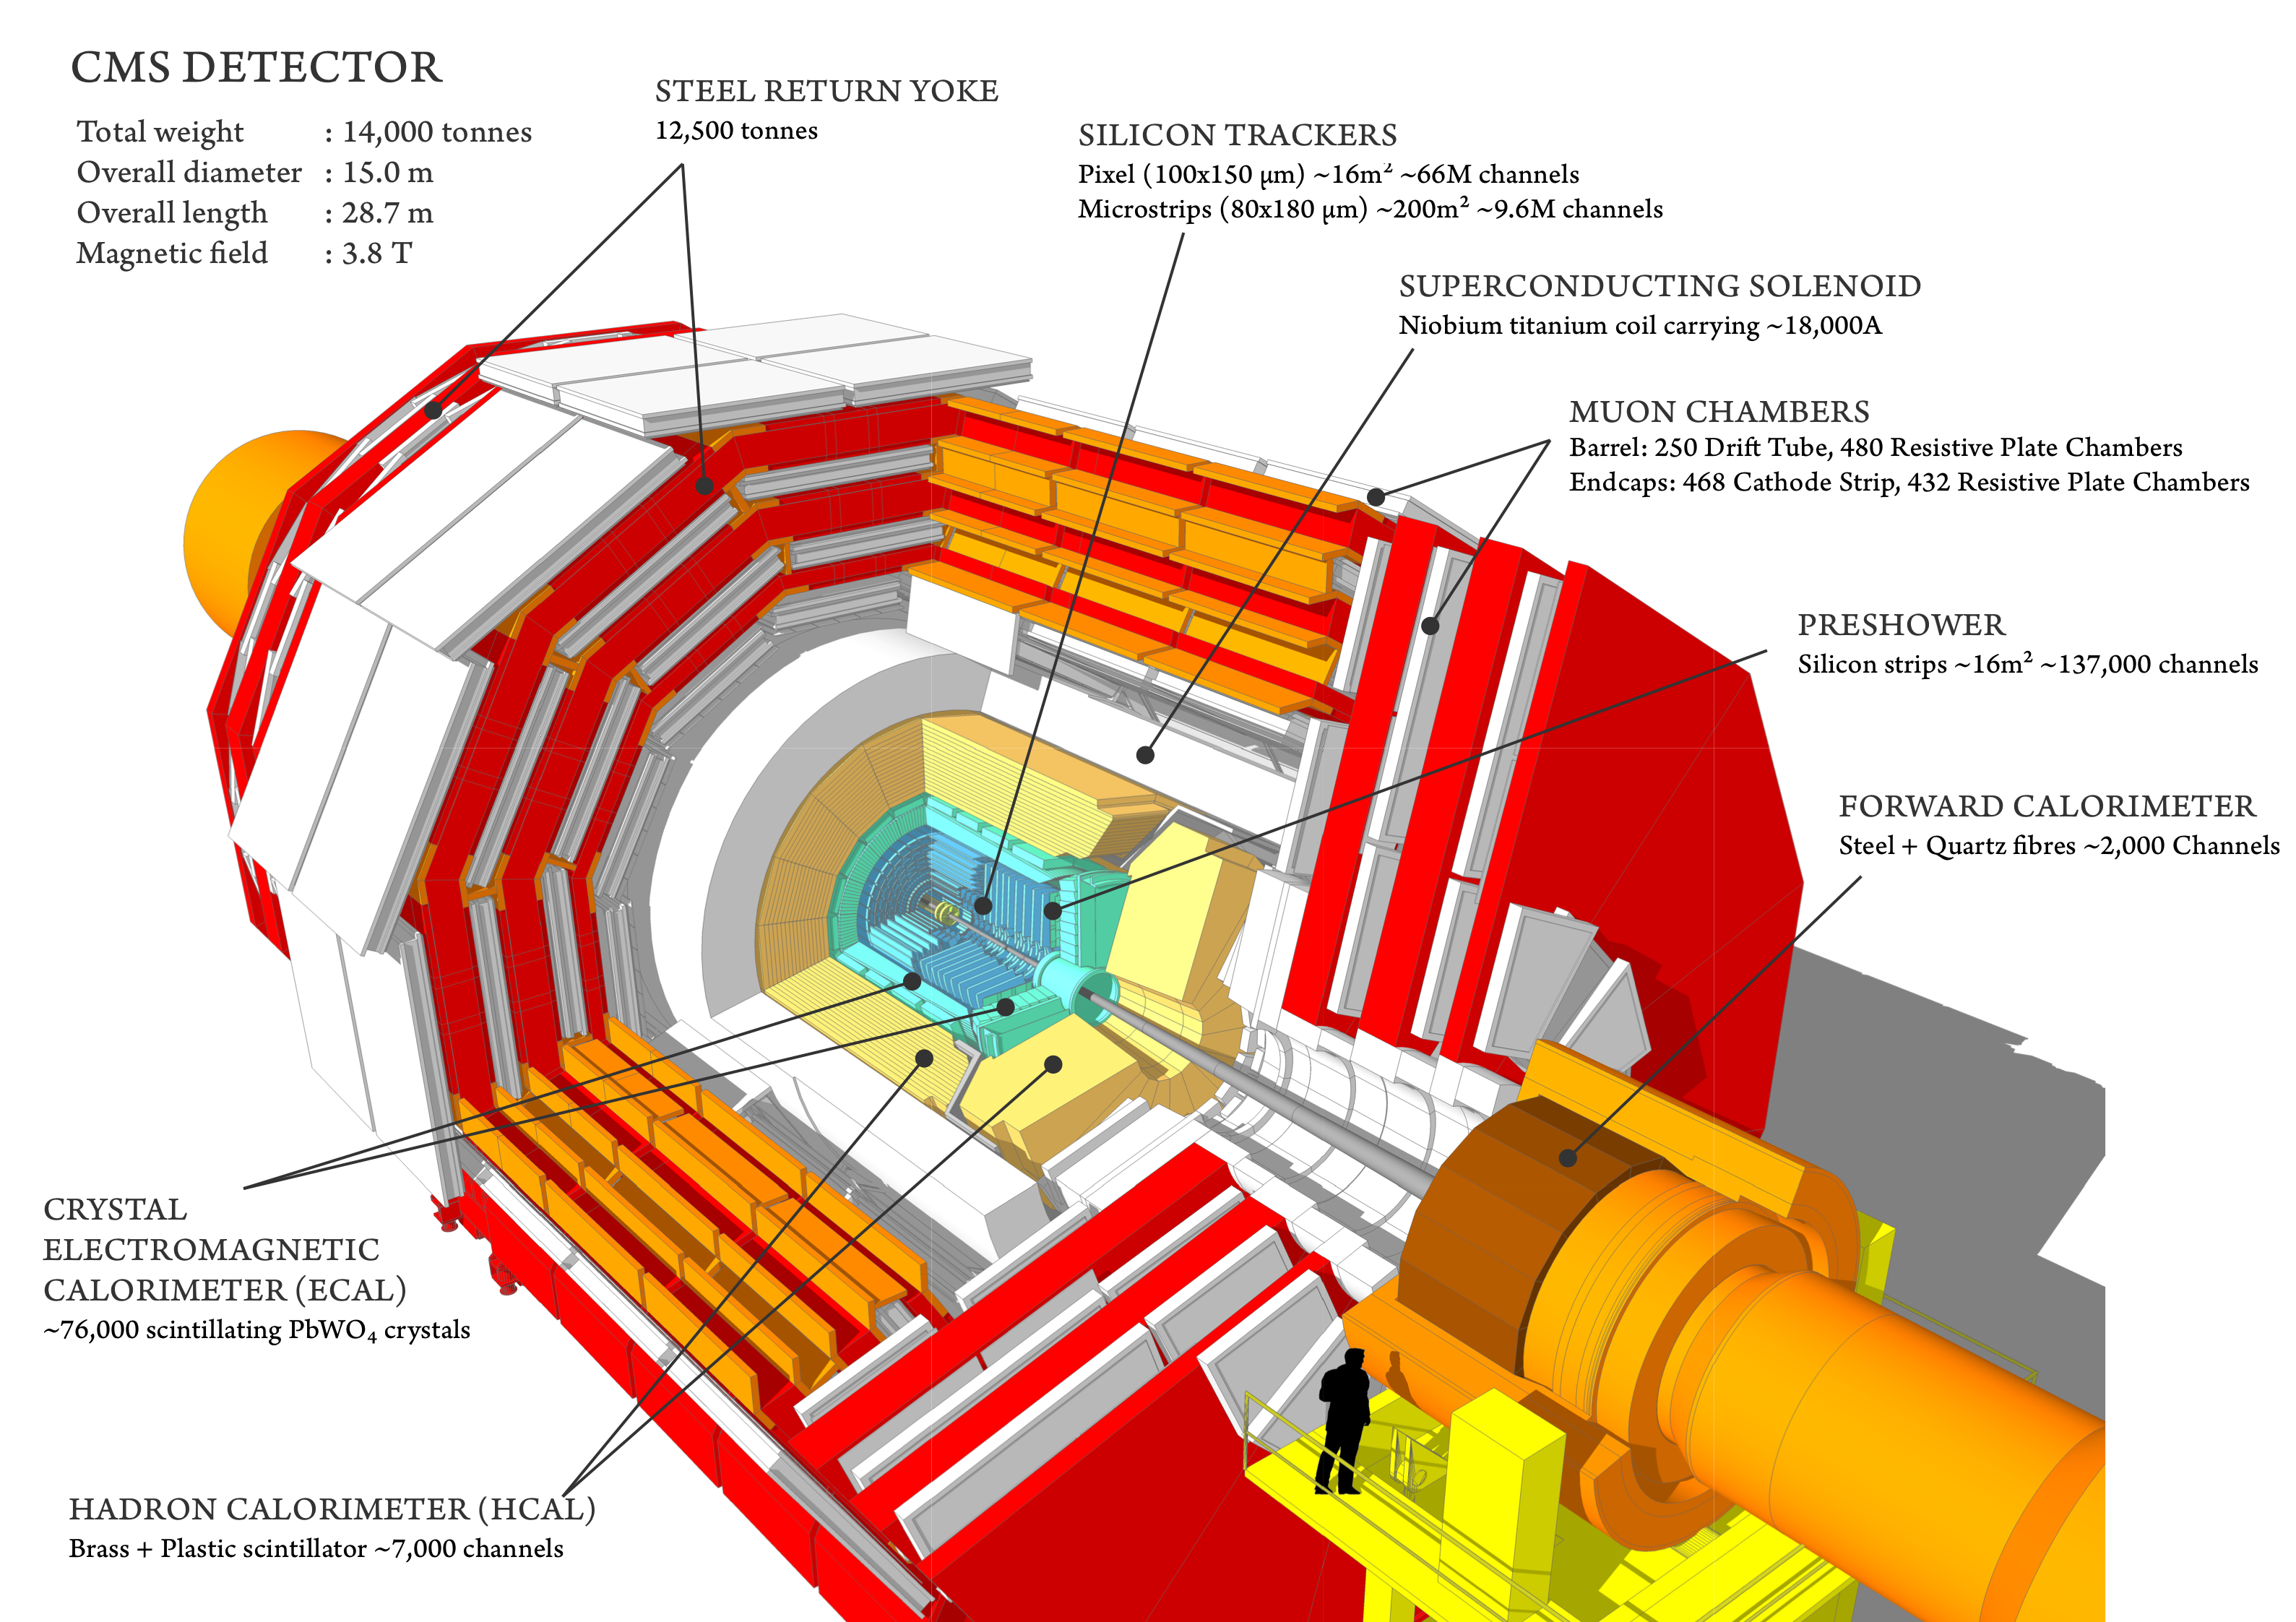
\includegraphics[width=.95\textwidth]{pics/cut_away_view}
\end{center}
\caption{The CMS Detector with inner components exposed and a person for scale.\label{fig:cms_onion}}
\end{figure}


\begin{figure}
\begin{center}
\includegraphics[width=.95\textwidth]{pics/CMSslice}
\caption{A slice of the CMS detector showing particle interactions with the various
sub-detectors. \label{fig:cms_transverse}}
\end{center}
\end{figure}


The Compact Muon Solenoid (CMS) Detector (Figures \ref{fig:cms_onion} and \ref{fig:cms_transverse}) is a general-purpose detector consisting of 
an all silicon tracker, a precision electromagnetic calorimeter (ECAL), a hadron calorimeter
 (HCAL), a 4 T superconducting solenoid and muon chambers. The solenoid deflects charged
 particles whose paths are traced in the tracker, making it possible to 
reconstruct the particle's momentum. The two calorimeters reconstruct the energy 
of and identify photons, electrons and hadronic jets.
The detector has cylindrical symmetry about the
 interaction point where the proton beams collide. By maintaining near full coverage 
of the interaction point, it is possible to detect signatures such as neutrinos or other 
weakly interacting particles as missing energy. 


\section{CERN Laboratory and the LHC}

CERN Laboratory is located on the border between Switzerland and France where the local language is French. Accordingly,
the lab name is an acronym in french ``Conseil Europ\'een pour la Recherche Nucl\'eaire'' or in English, ``European
Council for Nuclear Research''. Founded in 1954 as a collaborative project across 12 countries in Western 
Europe, the project has grown to 22 member states in 2017. The name is derived from the study 
fundamental physics, which at the time was nuclear physics.

The lab consists of numerous experiments studying fundamental physics \cite{experiments}, 
the largest of which are related to the
Large Hadron Collider which delivers proton-proton (as well as lead-lead) collisions to four
experiments: ATLAS, CMS, ALICE, and LHCb. Non-LHC experiments often utilize pieces of the accelerator
complex like the Super Proton Synchrotron (SPS) and the Proton Synchrotron (PS) to perform experiments 
where a single accelerator beam collides with a fixed target. There are groups
which study anti-matter and experiments investigating cosmic rays.

Although the United States is large contributor of technology
and person power, they are currently not a member state of CERN.
There is no provision that requires member states to be European
 (Israel is currently a member state). One will also not find
an official statement by the US or CERN as to why such a large contributor to the experiment
is not a member. While the US is not excluded from participation 
in the experiment, it does pose significant barriers for American scientists 
trying to obtain positions at CERN.  While I consider these decisions 
largely political in nature, I consider it worthwhile
to look  at the financial commitments member states make
 and what comparable US contributions would look like if the contributions were similar.
\begin{center}
\begin{table}[]
\begin{center}
\caption{A summary of the GDP, CERN lab contribution, and the ratio between GDP and the absolute contribution 
by country}
\begin{tabular}{cccc}
\textbf{Country} & GDP & Abs (Rel) Cont. & (Cont/GDP) $\times 10^{-7}$ \\
\hline
Germany & \$3.36T  & 231M CHF (20.5\%) & 6.8 CHF/USD  \\
France  & \$2.24T  & 170M CHF (15.1\%) & 7.5 CHF/USD\\
UK      & \$2.86T  & 161M CHF (14.3\%) & 5.6 CHF/USD\\
Italy   & \$1.82T  & 125M CHF (11.1\%) & 6.9 CHF/USD\\
Spain   & \$1.19T  & 88M  CHF (7.82\%) & 7.4 CHF/USD\\
\hline
USA     & \$18.03T & -             & -     
\end{tabular}
\end{center}
\label{tab:gdpcontrib}
\end{table}
\end{center}
\begin{center}
\begin{table}[]
\begin{center}
\caption{Differences in Absolute NNI vs GDP for the year 2015. Countries are ordered by absolute 
contribution size from highest to lowest. }
\begin{tabular}{ccccc}
\textbf{Country} & \textbf{GDP [USD]} & \textbf{NNI [USD]} &  \textbf{NNI/GDP} & \textbf{NNI/Capita}    \\
\hline
Germany & 3.36T & 3.31T & 0.99 & 40.6k\\
France  & 2.24T & 2.27T & 1.01 & 34.4k\\
UK      & 2.86T & 2.33T & 0.81 & 35.8k\\
Italy   & 1.82T & 1.84T & 1.01 & 30.3k\\
Spain   & 1.19T & 1.33T & 1.12 & 28.6k\\
\hline
USA     & 18.03T & 15.67 & 0.87 & 48.7k\\
\label{tab:nnicontrib}
\end{tabular}
\end{center}
\end{table}
\end{center}
The CERN operating budget provided by the individual member states (Table \ref{tab:nnicontrib}) 
The total budget for CERN in 2015 was 1127 Million Swiss Francs \cite{budget}. 
The USD/CHF exchange rate as of January 1, 2016 was 0.994 and 0.999 as of December 31, 2015. 
Countries contributing less than 5\% are excluded from the list (Switzerland contributes 3.87\%). 
The average contribution from the top 5 countries which comprise 68.8\% of the operating
budget is 0.068 million Swiss franc per billion USD of gross domestic product. 
For the United States, a comparable contribution (1224 Million USD) would be larger 
than the 2015 operating budget. If contributions were renormalized such that the total budget
were fixed, the United States would be funding more than half of the lab's operations. 

The contributions although nearly scaling linearly with GDP are defined by the CERN financial committee in 
terms of a related economic indicator NNI \cite{contribcalc} \cite{contribcalc2015}.  
The scale for each countries contribution is set by:
\begin{quote}
``Using the arithmetic average of three years of Net National
Income values until year before last year and applying the corresponding annual average
exchange rate for each year''
\end{quote}
The NNI is calculated as the Net National Product (NNP) less Indirect taxes. Indirect taxes are taxes which are
collected by an intermediary from the person bearing the ultimate burden of the tax (sales tax, value added tax, 
ect). The Net National Product is the Gross National Product (GNP) less depreciation, the decrease in value of 
assets or the allocation of the costs of an asset to a later period in which the asset is used. The GNP was
once a more common measure of economic activity than GDP, and is closely related. GNP is equal to GDP plus the
income earned by residents from overseas investment and less the income earned within the domestic economy by overseas residents. We thus write NNI as a function of GDP:
\begin{align*}
\text{NNI} &= \text{GDP} + (\text{Resident income from overseas investment})\\
 &- (\text{Depreciation}) - (\text{Indirect taxes}) - (\text{Domestic income by overseas residents})
\end{align*}
The Net National Income (NNI) is listed for the top contributors for the year 2015 in Table \ref{tab:nnicontrib}. 
Net national income is defined as the net national product minus indirect taxes. 
For most countries, GDP/NNI is nearly 1, the exceptions being the UK and Spain. Had the contributions
been scaled by GDP, the UK would be paying significantly more and Spain somewhat less. Spain, to have a 
GDP/NNI ratio greater than 1 must have significant component of income earned by residents from oversea
investment. 

\subsection{The Large Hadron Collider}

\begin{figure}
\begin{center}
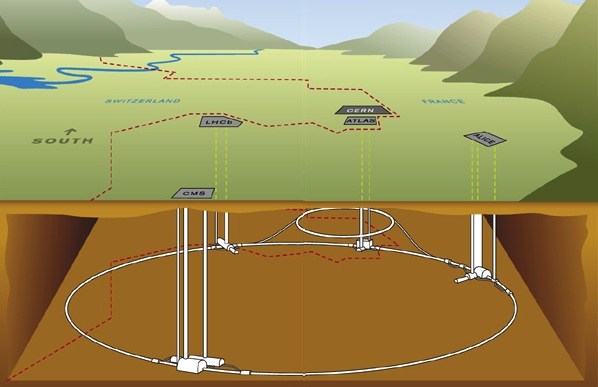
\includegraphics[width=.7\textwidth]{lhc_tunnel}
\caption{The LHC tunnel installed on the border of Geneva, Switzerland and France. 
The experiments are distributed along the circumference of the ring. \label{fig:tunnels}}
\end{center}
\end{figure}

\begin{figure}
\begin{center}
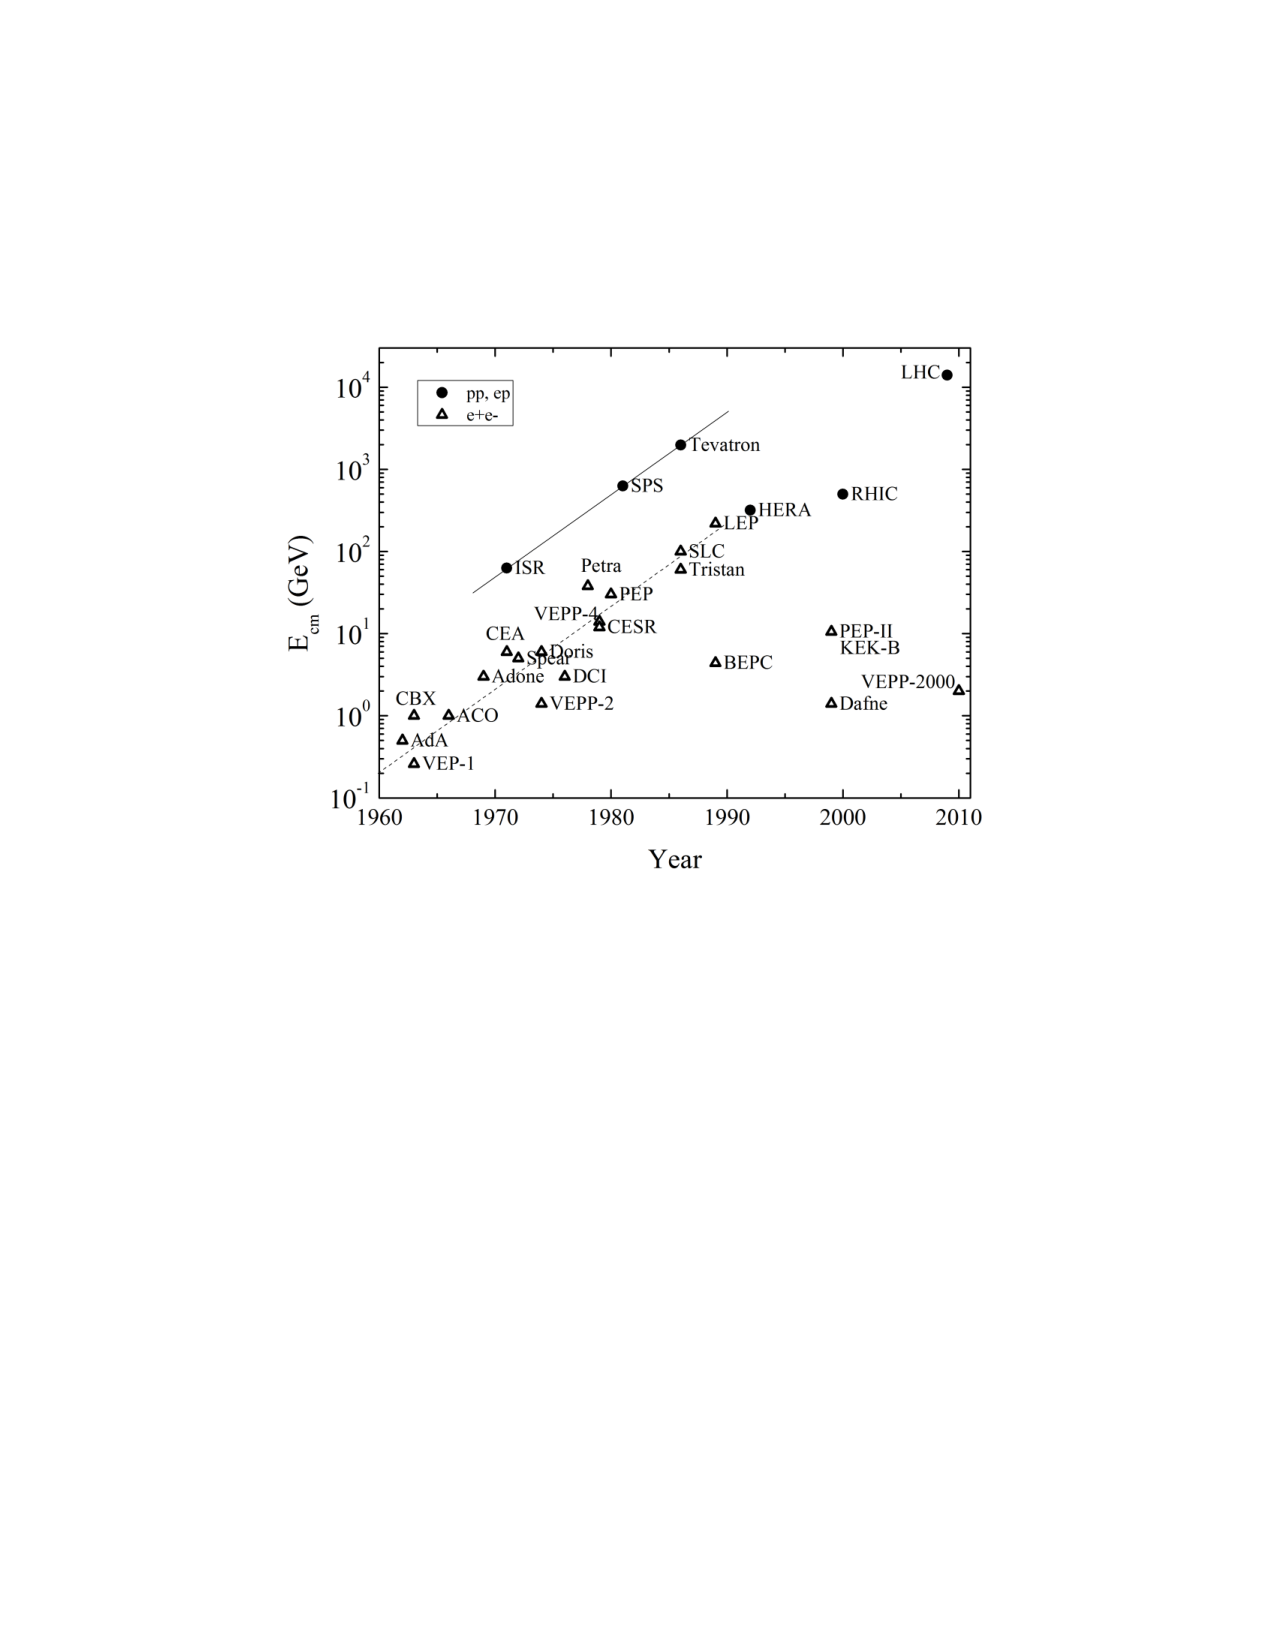
\includegraphics[width=.75\textwidth]{pics/collider_energies}
\caption{The historical progression of collider energies in time.\label{fig:colliders}}
\end{center}
\end{figure}

\begin{center}
\begin{table}[]
\begin{center}
\caption{LHC Running Parameters \cite{lhcparams}}
\begin{tabular}{ccc}
\textbf{Parameter} & \textbf{Value} & \textbf{Remarks} \\
\hline
Circumference (km) & 26.7 km & 100-150 m underground\\
Number of Dipoles & 1232 & Nb-Ti Cables \\
Length of Dipole & 13.3 m & \\
Dipole Field Strength & 8.4 T & Results form high beam energy \\
Operating Temperature & 1.9 K & He cooled superconducting magnets\\
Current in Dipole Coils & 13kA & Results from high magnetic field \\
Beam Intensity & 0.5 A & \\ 
Beam Stored Energy & 362 MJ & 1MJ melts 2kg Cu \\
Magnet Stored Energy / octant & 1100 MJ & \\
\end{tabular}
\end{center}
\end{table}
\end{center}


The Large Hadron Collider (LHC) is a 27 kilometer ring 100m underneath the border of Geneva, Switzerland and France 
(Figure \ref{fig:tunnels}). It is the largest and most powerful particle collider of the world at a design
instantaneous luminosity of $10^{34}$ cm$^{-2}$s$^{-1}$ and $\sqrt{s}=$13 TeV (Figure \ref{fig:colliders}). 
The previous highest energy collider, Tevatron, a proton anti-proton collider, operated at $\sqrt{s}=1.96$ TeV 
and an upgraded instantaneous luminosity of $4\times 10^{32}$ cm$^{-2}$s$^{-1}$. 

The LHC consists of a series of super conducting
magnets that steer two beams of protons about the circumference and focus them at collision points where the
experiments are located. The bunches of protons in the LHC are bent into a circular trajectory by more than 1200
 superconducting dipole magnets and are focused and maintained close to the ideal
 orbit around the ring by hundreds of superconducting quadrupole magnets. 
Thousands of corrector magnets around the ring allow the beam to be steered closer 
to the ideal orbit, make the focusing independent of the particle's energy variations
 within a bunch, and cancel the effects of higher order multipoles in the fields induced 
by small field imperfections in the main magnets. 
The radio frequency (RF) field in superconducting cavities is placed periodically around 
the ring and accelerates the protons from the injection energy of 450 GeV to the final
 operating energy, which is designed to be 7 TeV per beam. The RF field also causes the
 protons to be bunched, as only particles at or near a certain equilibrium phase on 
the RF wave will be accelerated stably. Special quadrupoles around each interaction region
 focus the bunches down to a small transverse size, to increase the likelihood of a
 proton-proton collision each time two bunches pass through each other.

The instantaneous luminosity delivered by the large hadron collider
 can be determined from  the following expression:
\begin{equation}
L = \frac{f}{\pi} \frac{N_p N_{p`}}{n_b} \frac{\gamma}{\sqrt{\beta^*_x \beta^*_y E_x^* E_y^*}}
\end{equation}
\begin{itemize}
\item $f$: revolution frequency of the beams. 
\item $N_p$ the number of protons in the beam
\item $n_b$ the number of proton bunches 
\item $\beta^*_{x,y}$ the transverse wavelengths of the betatron oscillations
\item $E_{x,y}^*$ the transverse emittance of the beams
\item $\gamma$: relativistic factor
\end{itemize}
To increase luminosity and correspondingly the total amount of data taken in a fixed time interval,
 this parameterization tells us we want a high frequency of collisions, high proton density within 
the bunches, small oscillations transverse to the ideal path, and a small average
spread in position momentum space. The small spread in phase space (low emittance) 
means the particles are confined to a small area and have roughly the same
 momentum. This result in a high probability of interaction.
%% \begin{figure}
%% \begin{center}
%% 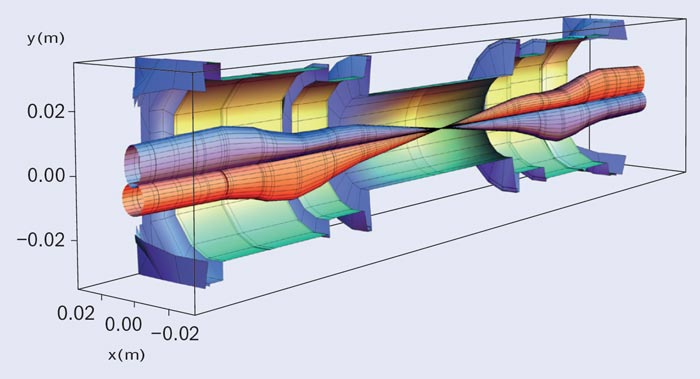
\includegraphics[width=.7\textwidth]{pics/beam_squeeze}
%% \caption{Squeeze}
%% \end{center}
%% \end{figure}

%% \begin{figure}
%% \begin{center}
%% 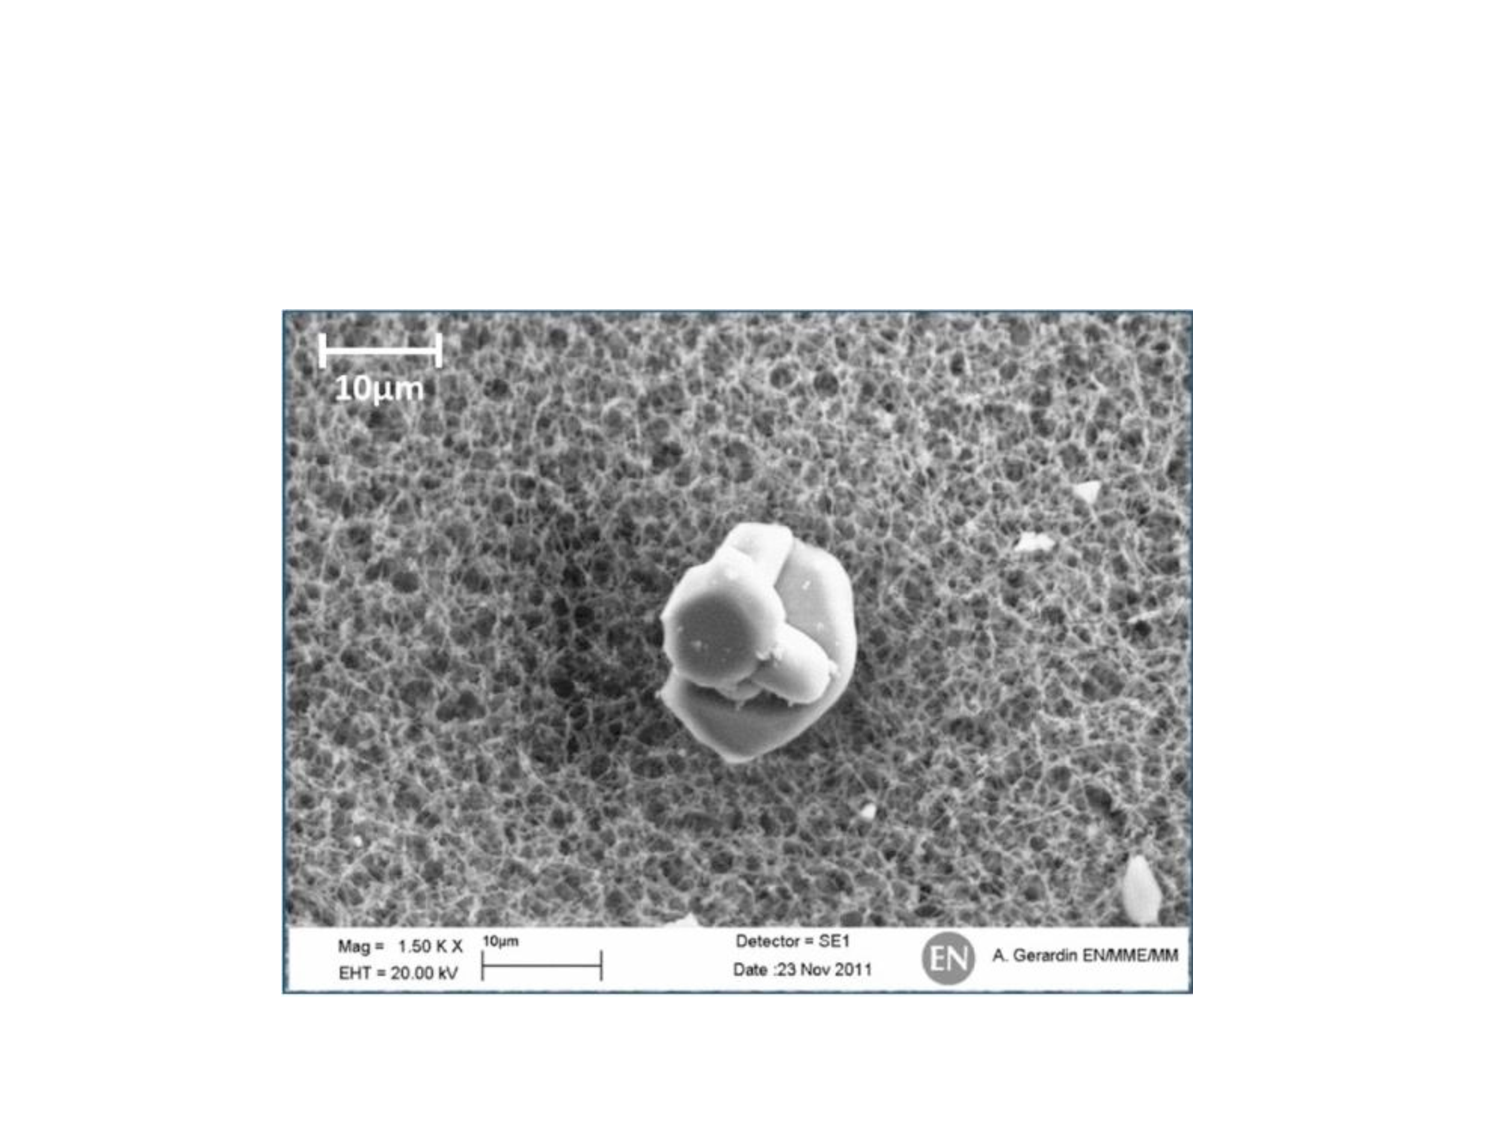
\includegraphics[width=.75\textwidth]{pics/dust}
%% \caption{Unidentified Falling Objects (UFOs)}
%% \end{center}
%% \end{figure}
\section{Superconducting Solenoid}

\begin{figure}
\begin{center}
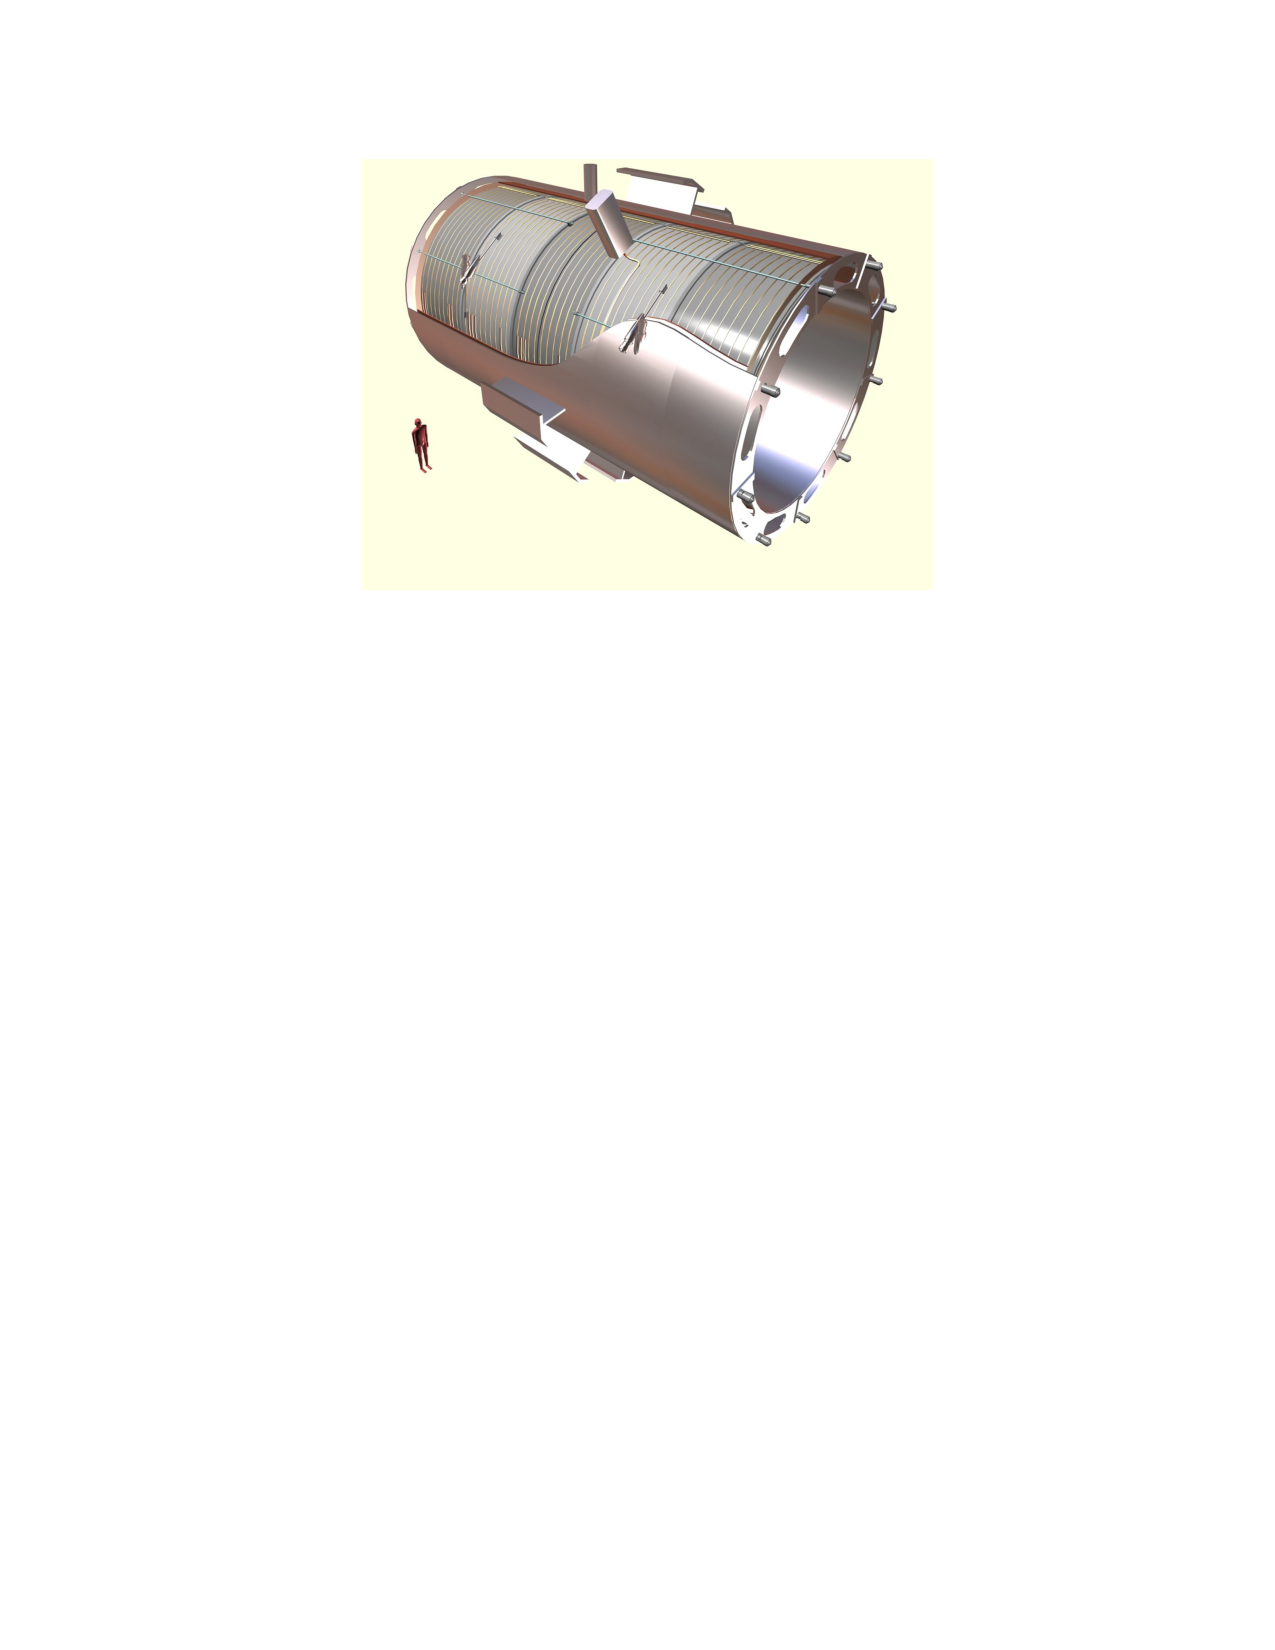
\includegraphics[width=.65\textwidth]{pics/solenoid_diagram}
\end{center}
\caption{The CMS solenoid with a human for scale.}
\label{fig:solenoid}
\end{figure}

\begin{figure}
\begin{center}
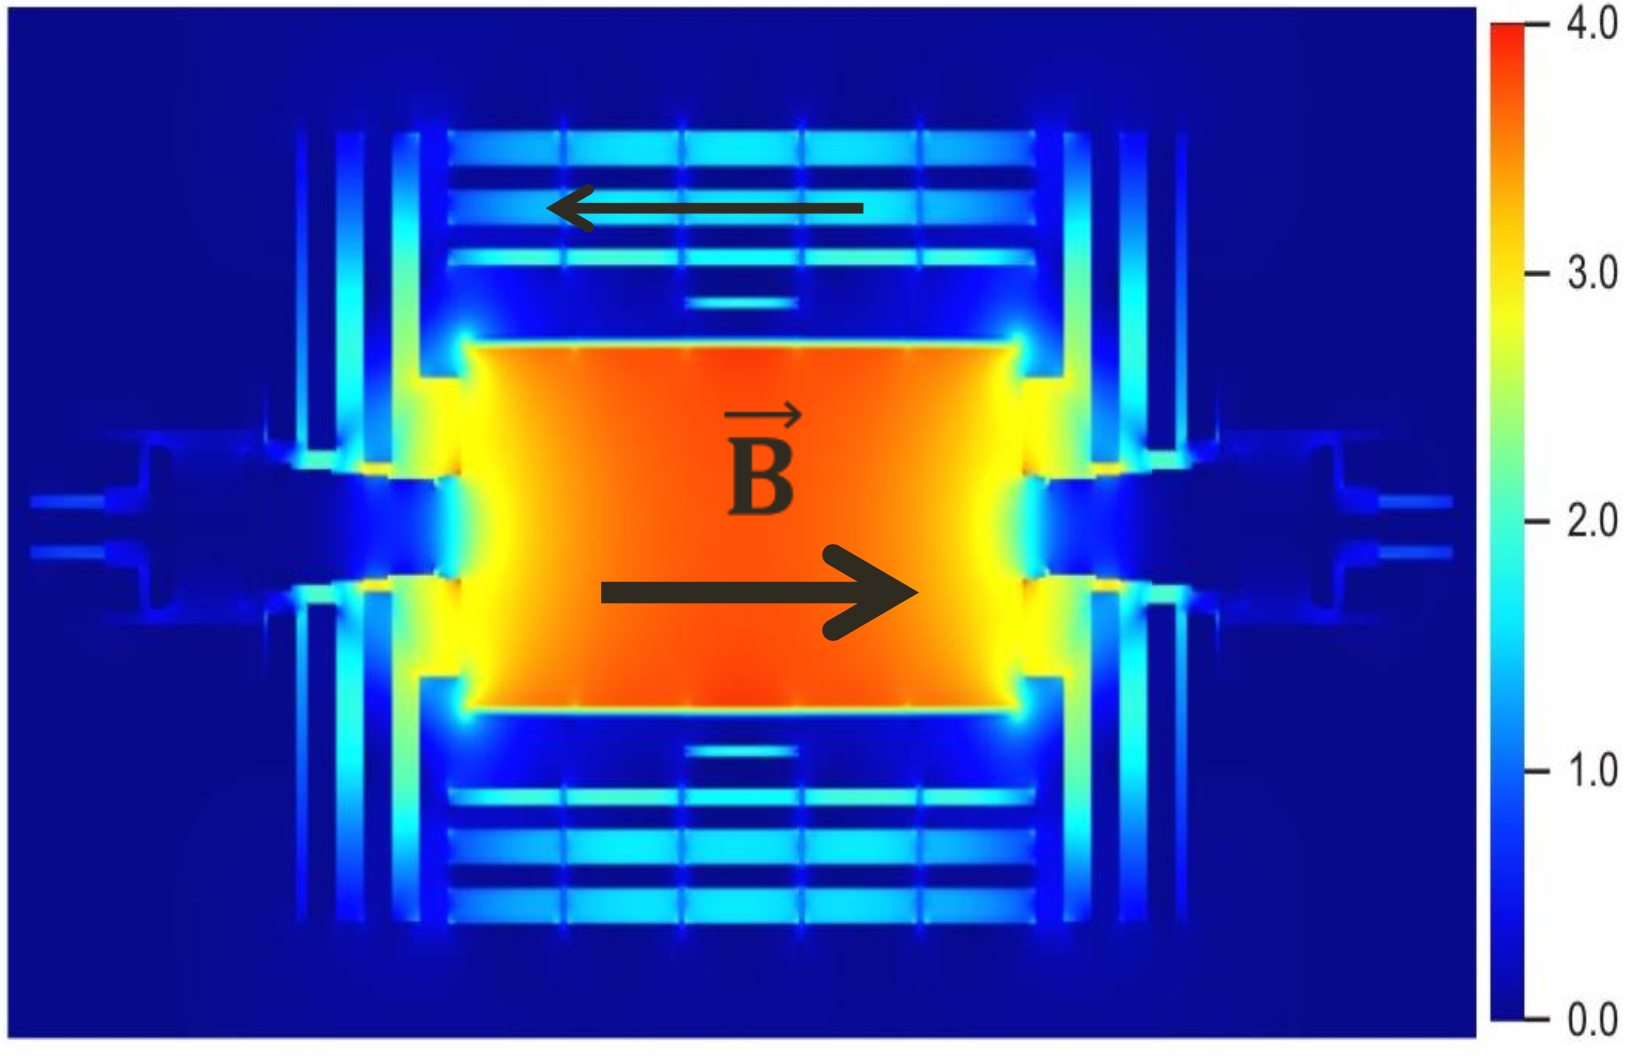
\includegraphics[width=.65\textwidth]{pics/b_field}
\end{center}
\caption{The CMS magnetic field in units of Tesla (T).}
\label{fig:solenoid_bfield}
\end{figure}

It is worth beginning this discussion around the central feature the rest of the detector is built, the 
4 T  superconducting solenoidal magnet. For scale, a typical refrigerator magnet is on the 
order of $10^{-2}$ T and the MRI magnets can range between 0.5-3.0 T. The magnetic field is used
to measure the momentum of charged particles by bending their trajectories. As the size of the bend is
proportional to the field and inversely to the momentum of the particle, a stronger field is required 
to measure higher energy particles with precision. 

\begin{figure}
\begin{center}
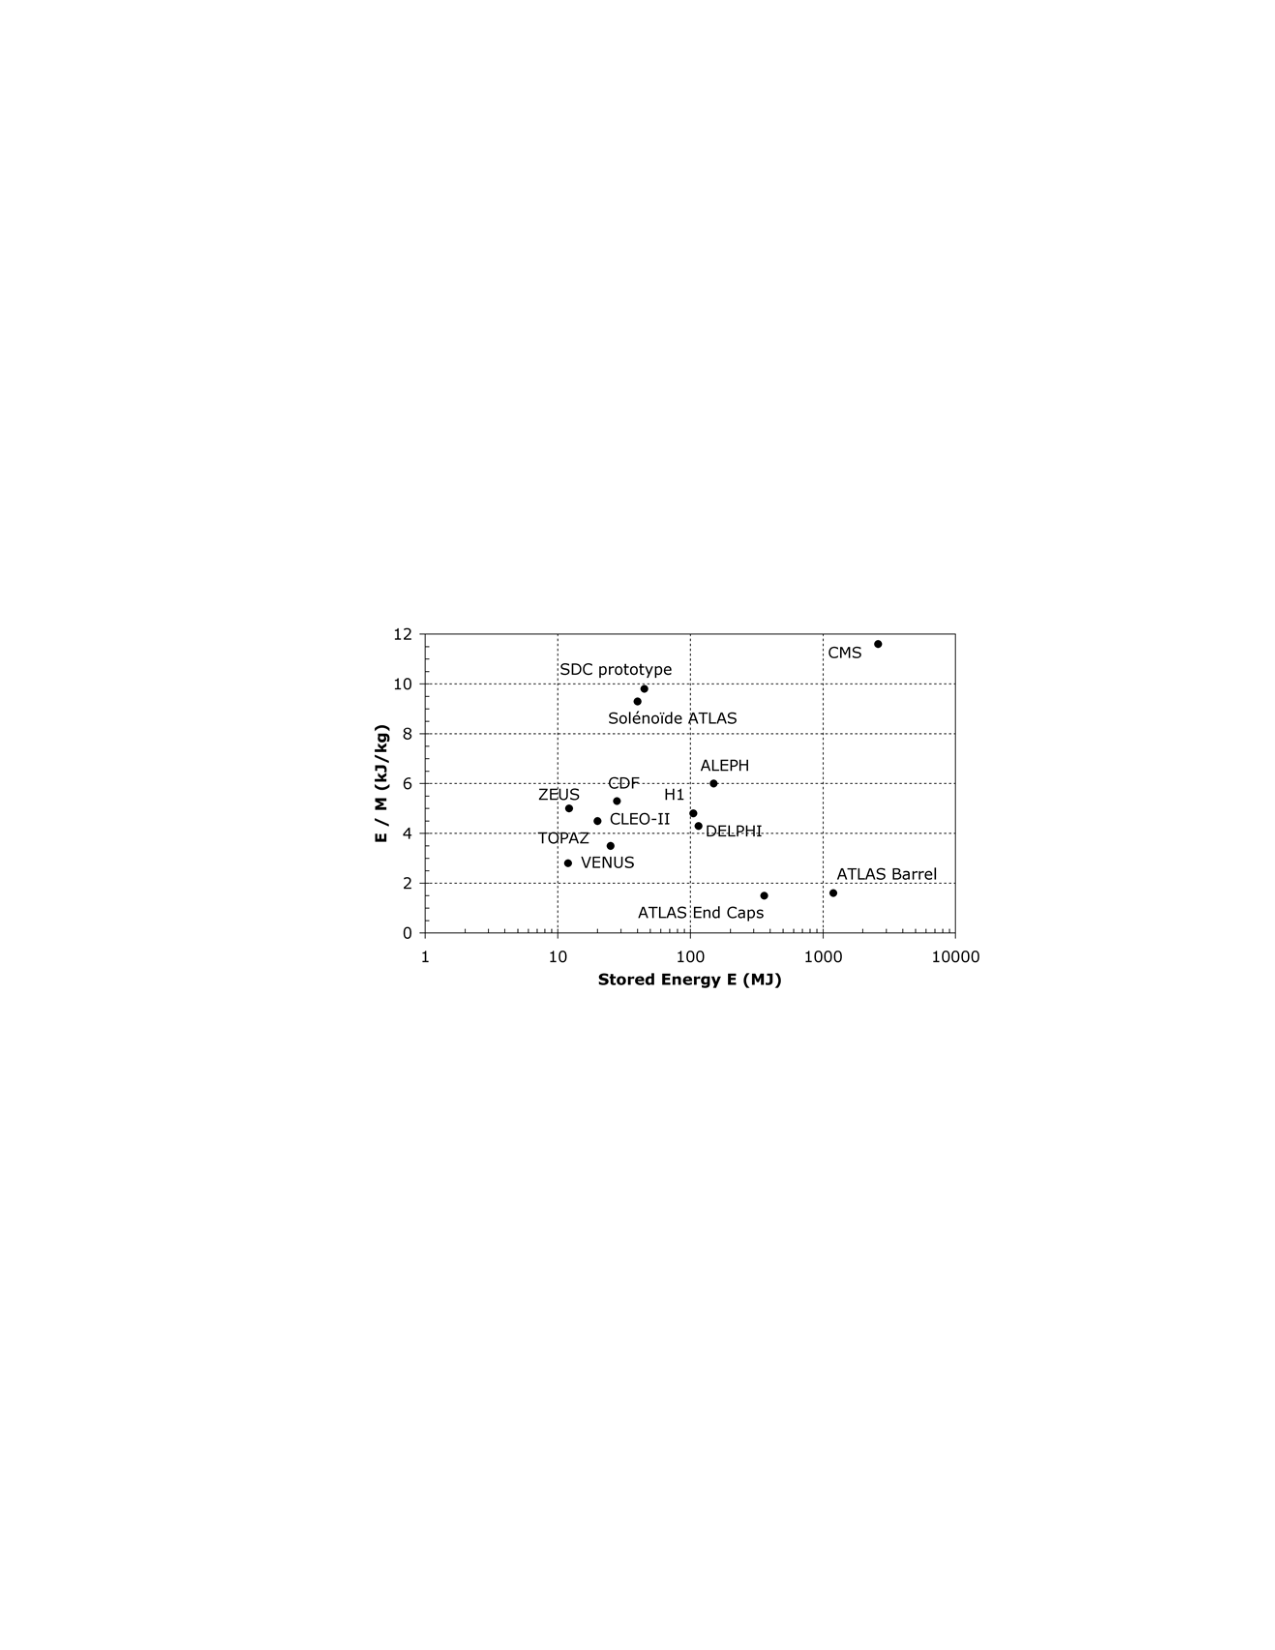
\includegraphics[width=.85\textwidth]{pics/CMS_EoverM}
\end{center}
\caption{The relationship of E/M and E for various collider experiments.}
\label{fig:eoverm}
\end{figure}

The magnet is 6 meters in diameter with 12.5 meters in length (Figure \ref{fig:solenoid}). The magnetic field (Figure \ref{fig:solenoid_bfield}) is generated 2180 turns wound in four layers of Niobium Titanium conductors inside an aluminum cylinder carrying a
 nominal current of 20 kA.  At the design field strength the solenoid a stores magnetic field of 
2.66 GJ, the largest stored energy of any magnet ever built. The energy to mass ratio is 11.6 kJ/kG a identifying 
feature in the historical context of detector magnets (Figure \ref{fig:eoverm}). The magnet is supplemented 
by a 10,000 ton iron return yoke which takes in the flux of the magnetic field from the solenoid improving
uniformity in the field.

\begin{figure}
\begin{center}
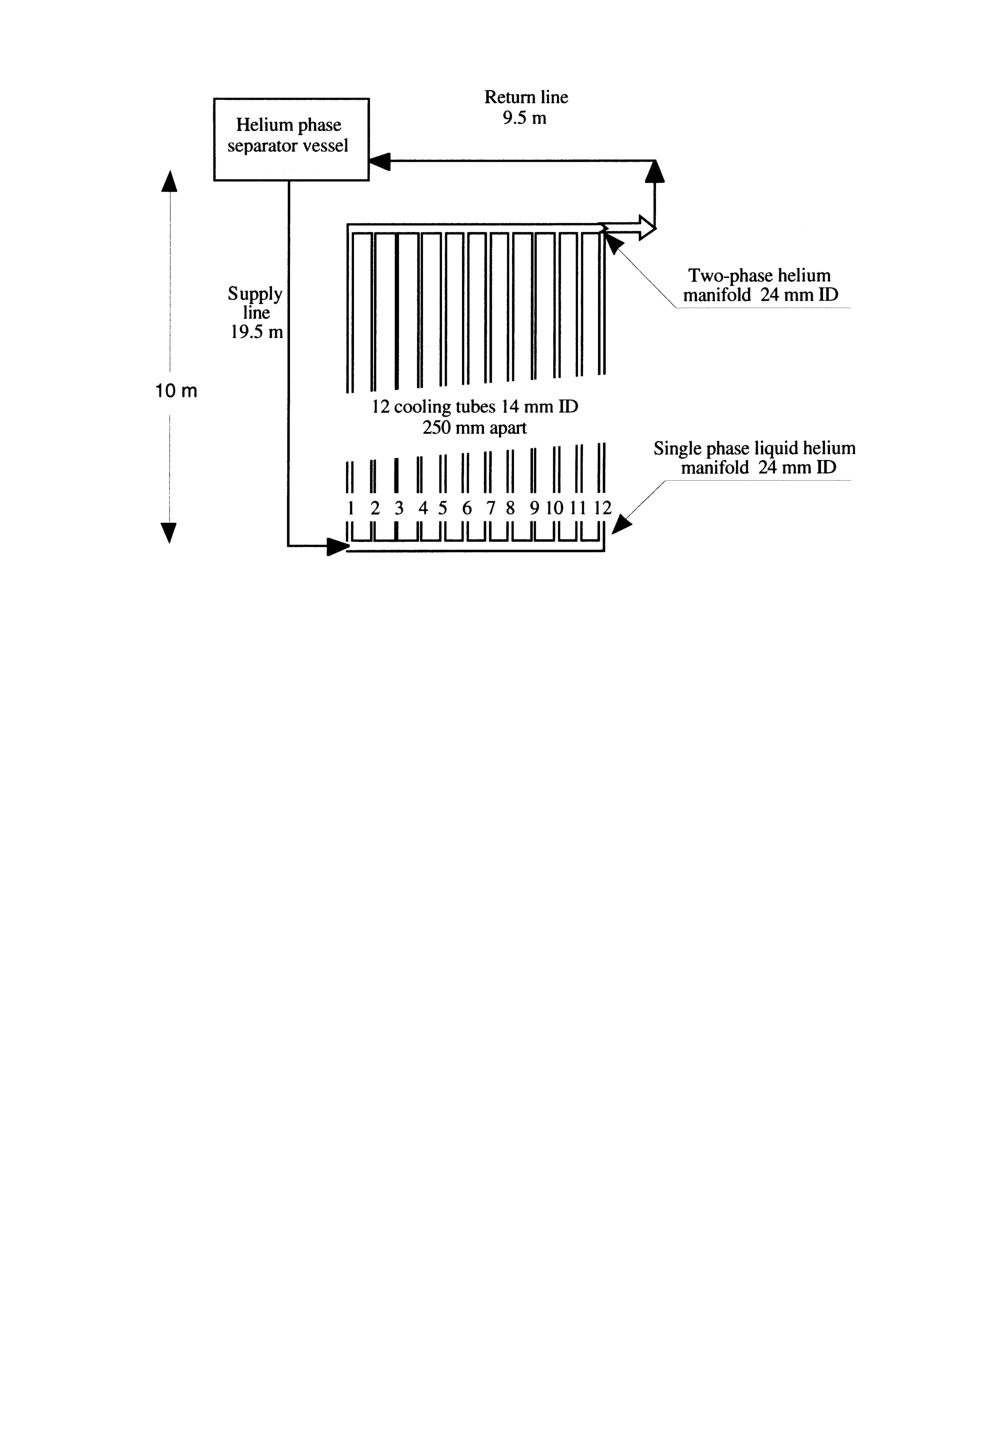
\includegraphics[width=.85\textwidth]{pics/thermosiphon}
\end{center}
\caption{A sub circuit of the CMS thermosiphon}
\label{fig:siphone}
\end{figure}

To operate in a superconducting state, the system is cooled to 4.5 K with a thermosiphon
\cite{quench}. This process  takes 3 days to achieve from room temperature.
A thermosiphon is an indirect cooling method utilizing passive heat exchange where,
rather than pumping the liquid helium, the flow is induced thermally (Figure \ref{fig:siphone}). 

\section{Electromagnetic Calorimeter (ECAL)}

\begin{figure}
\begin{center}
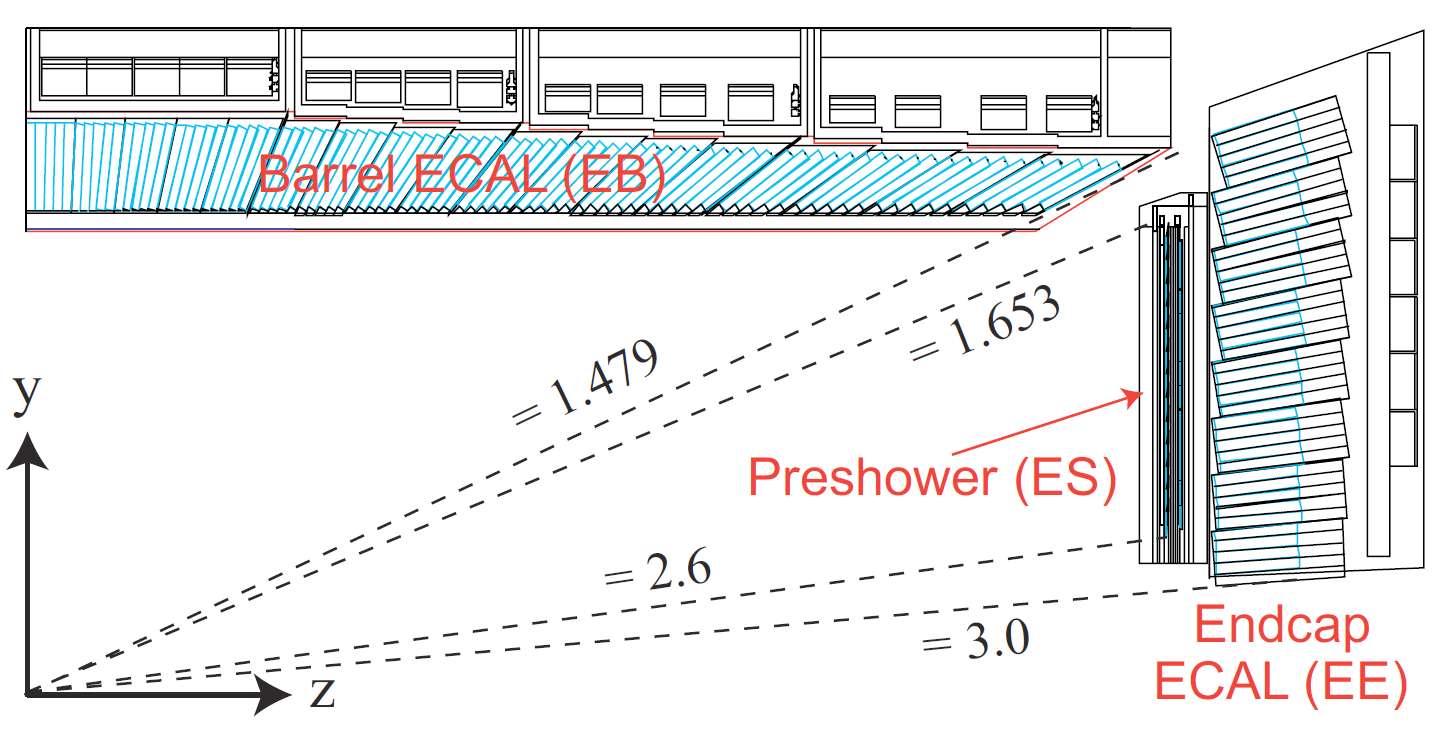
\includegraphics[width=.95\textwidth]{pics/ecal_diagram_side}
\end{center}
\caption{Kinematic coverage of the electromagnetic calorimeter (ECAL) barrel and endcap}
\label{fig:ecal}
\end{figure}

The electromagnetic calorimeter (ECAL) exists to measure the energy of electromagnetic
showers of electrons and photons. For high energy electromagnetic objects  above the mass threshold of 
pair production, $\gamma \rightarrow e^+e^-$, the interaction with matter occurs as an electromagnetic shower.
 In this shower, photons pair produce electron-positon pairs and
electrons undergo bremsstrahlung radiation: $e^\pm \rightarrow \gamma e^\pm$. This processes continues until 
the individual particles in the shower cannot continue $1\rightarrow 2$
 processes and instead undergo multiplicity preserving interactions such 
as Compton scattering and ionization.

The detector material (for CMS a scintillating crystal) is characterized by the shower's
 Moli\`ere Radius, defined as the radius
 transverse to the incidence of a cylinder that containing 90\% of the shower. For the CMS ECAL, 
crystals have approximately the Moli\`ere radius of approximately 2.2 cm. The material can further
be characterized by its radiation length, the typical amount of matter the incident particle
can traverse before an interaction. The CMS crystals have a relatively short radiation
 length of 0.9 cm. Each crystal is approximately 25 radiation lengths = 23 cm. 

The crystal energy resolution as a function of energy is characterized as:
\begin{equation}
\frac{\sigma(E)}{E} = \frac{S}{\sqrt{E}} \oplus \frac{N}{E} \oplus C
\end{equation}
Here $\sigma$ is the gaussian standard deviation of the energy measurement, the operator $\oplus$ signifies addition in quadrature, $S$ is 
the stochastic term, $N$ is the
electronic readout noise, and $C$ is the constant term which does not scale with energy. The 
stochastic term $S$ comes from the statistical nature of the photoelectric shower and the 
containment within the crystal. The readout term arises from the electronics noise in the preamplifier and digitization of the signal. The constant term $C$ is caused by non uniformities between
the many crystals and is ultimately dominated by the crystal to crystal inter calibration. As
the first two terms scale inversely with energy, the constant term is dominant for high energy photons and electrons $> 50$ GeV . 
The design energy resolution for high energy photons like those
found in the discovery of the Higgs bosom is $< 0.5\%$

\begin{figure}
\begin{center}
%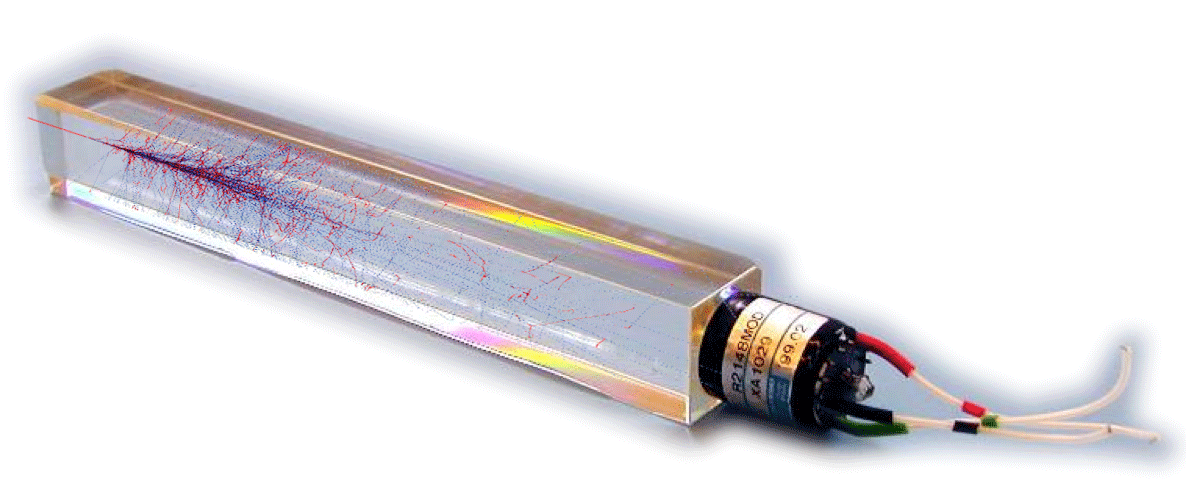
\includegraphics[width=.45\textwidth]{pics/ecal_crystal}
%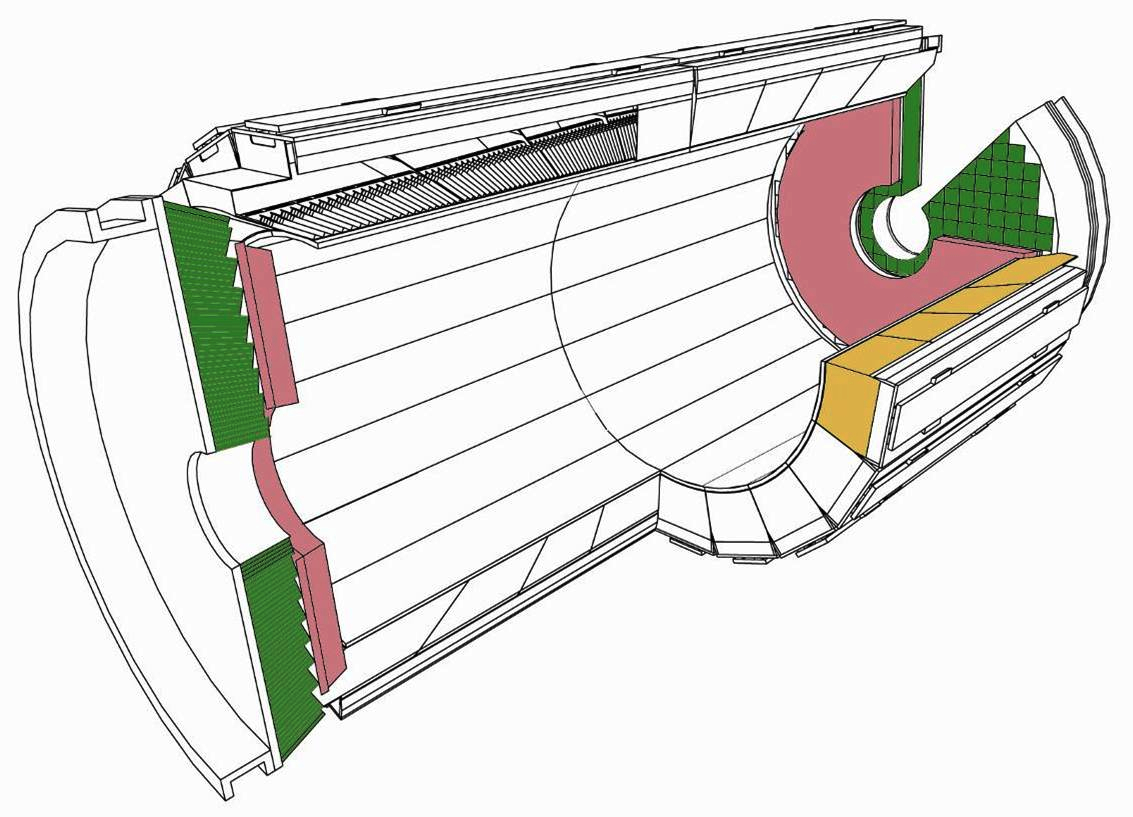
\includegraphics[width=.45\textwidth]{pics/ecal_diagram}
%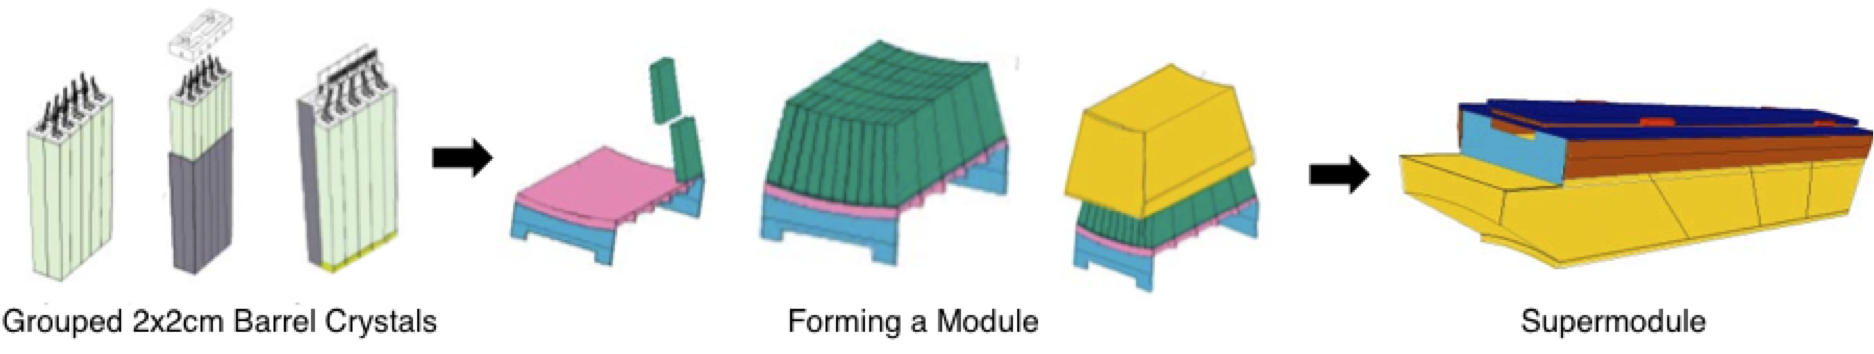
\includegraphics[width=.95\textwidth]{pics/Supermodule}
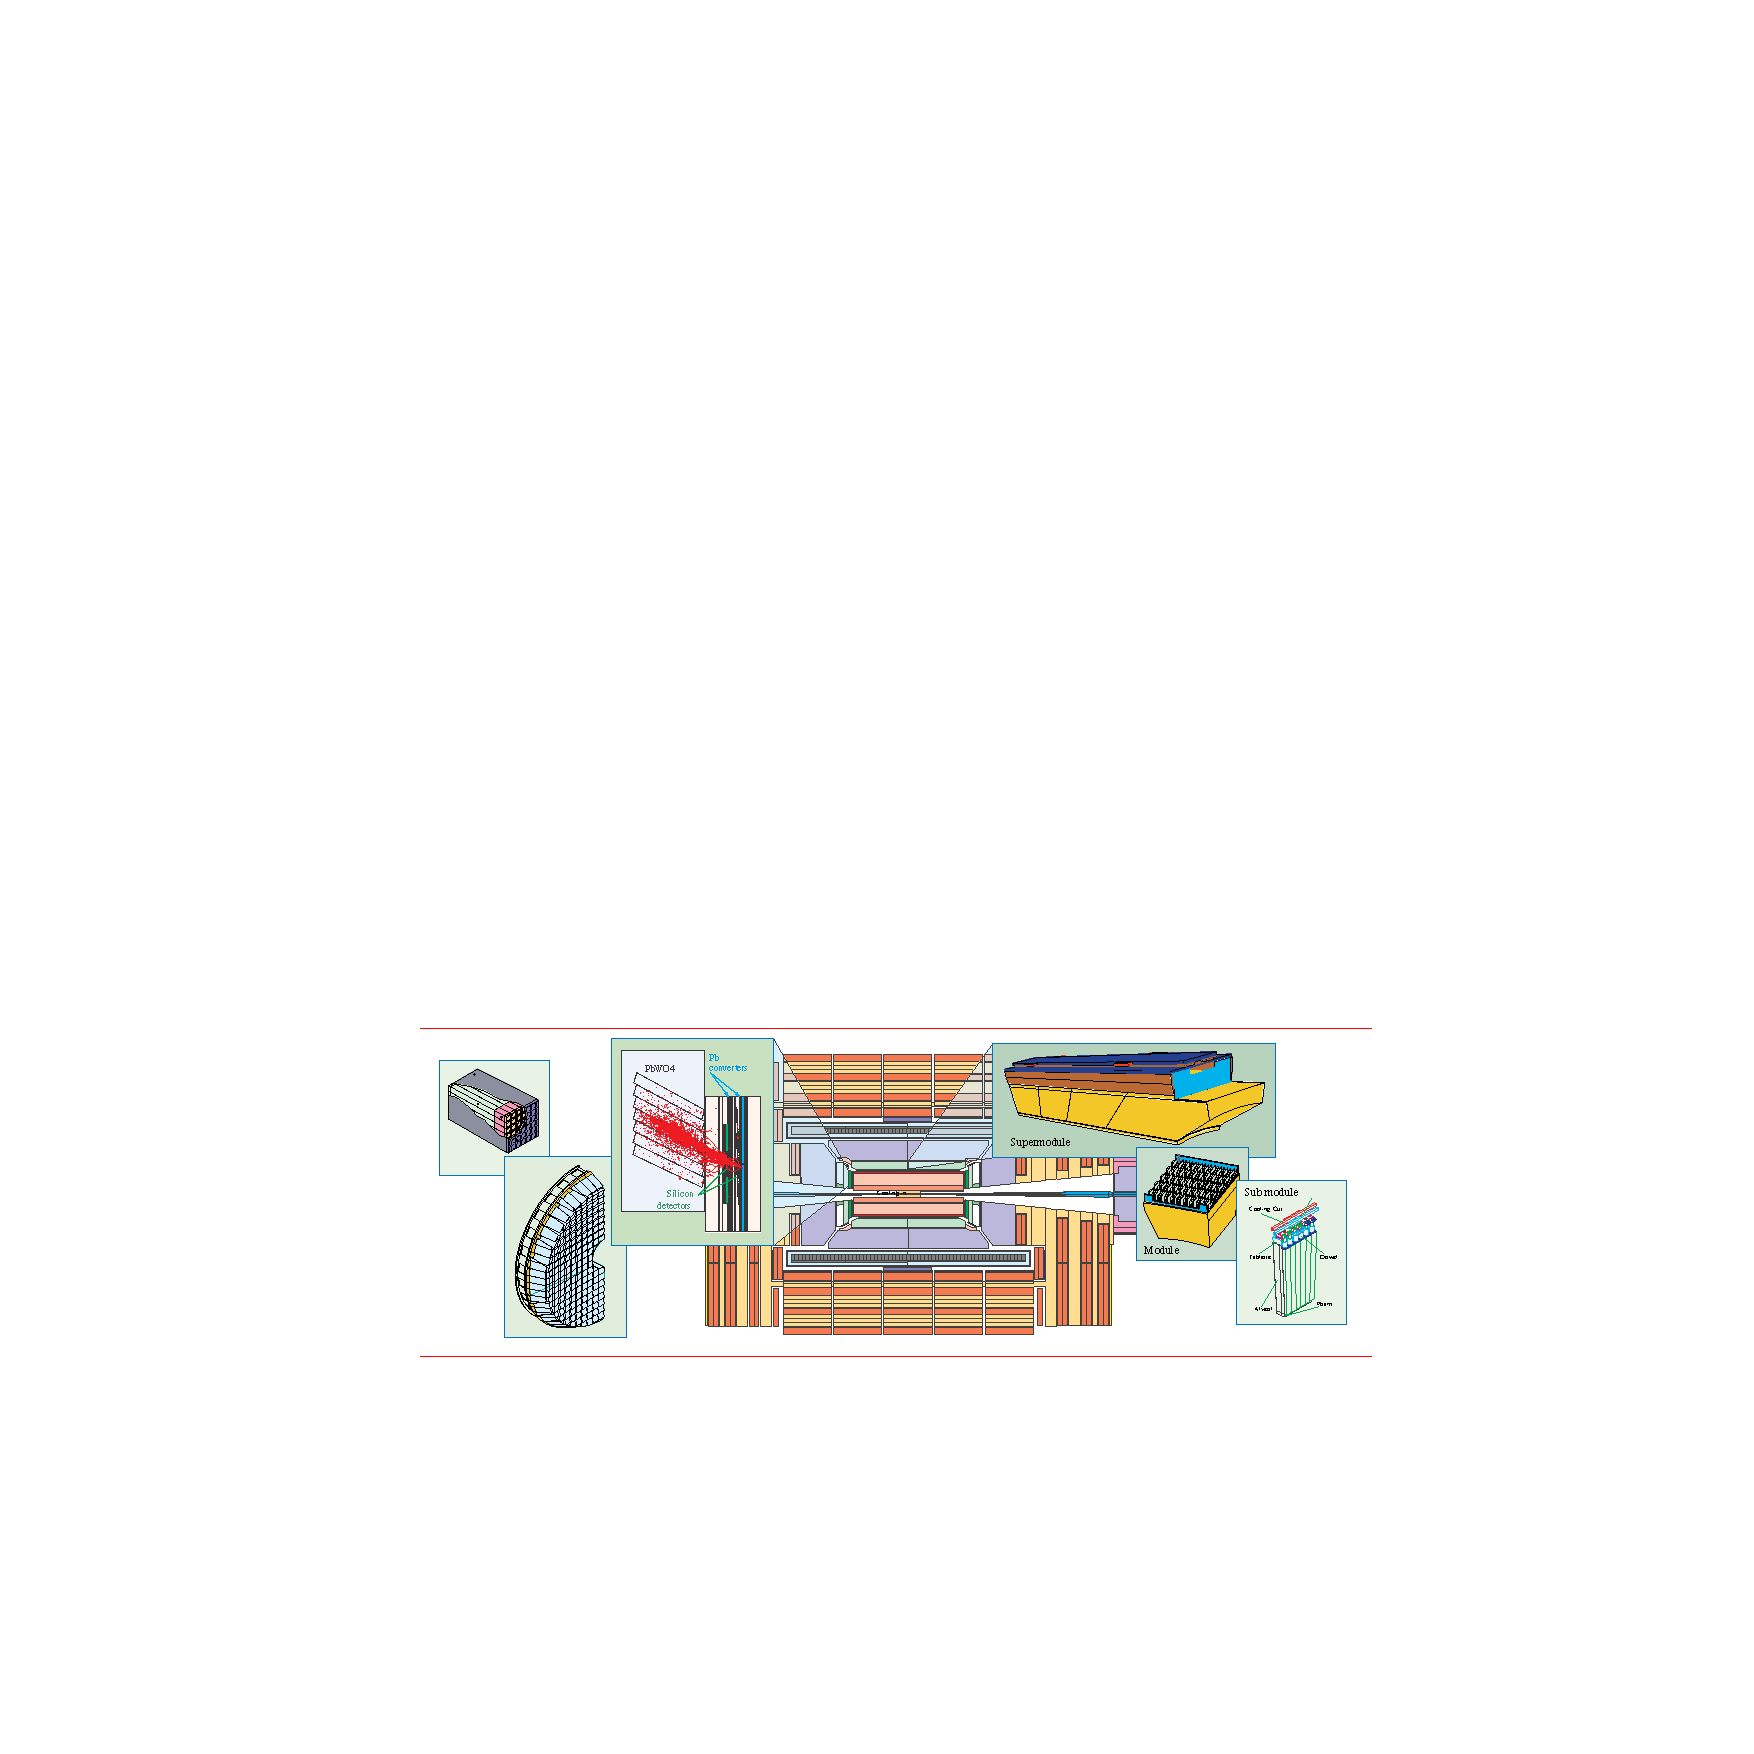
\includegraphics[width=.95\textwidth]{pics/cms_ecal_parts}
\end{center}
\caption{The CMS ECAL crystals as formed into sub modules, modules, supermodules and dees.}
\label{fig:ecal_crystal}
\end{figure}

\begin{figure}
\begin{center}
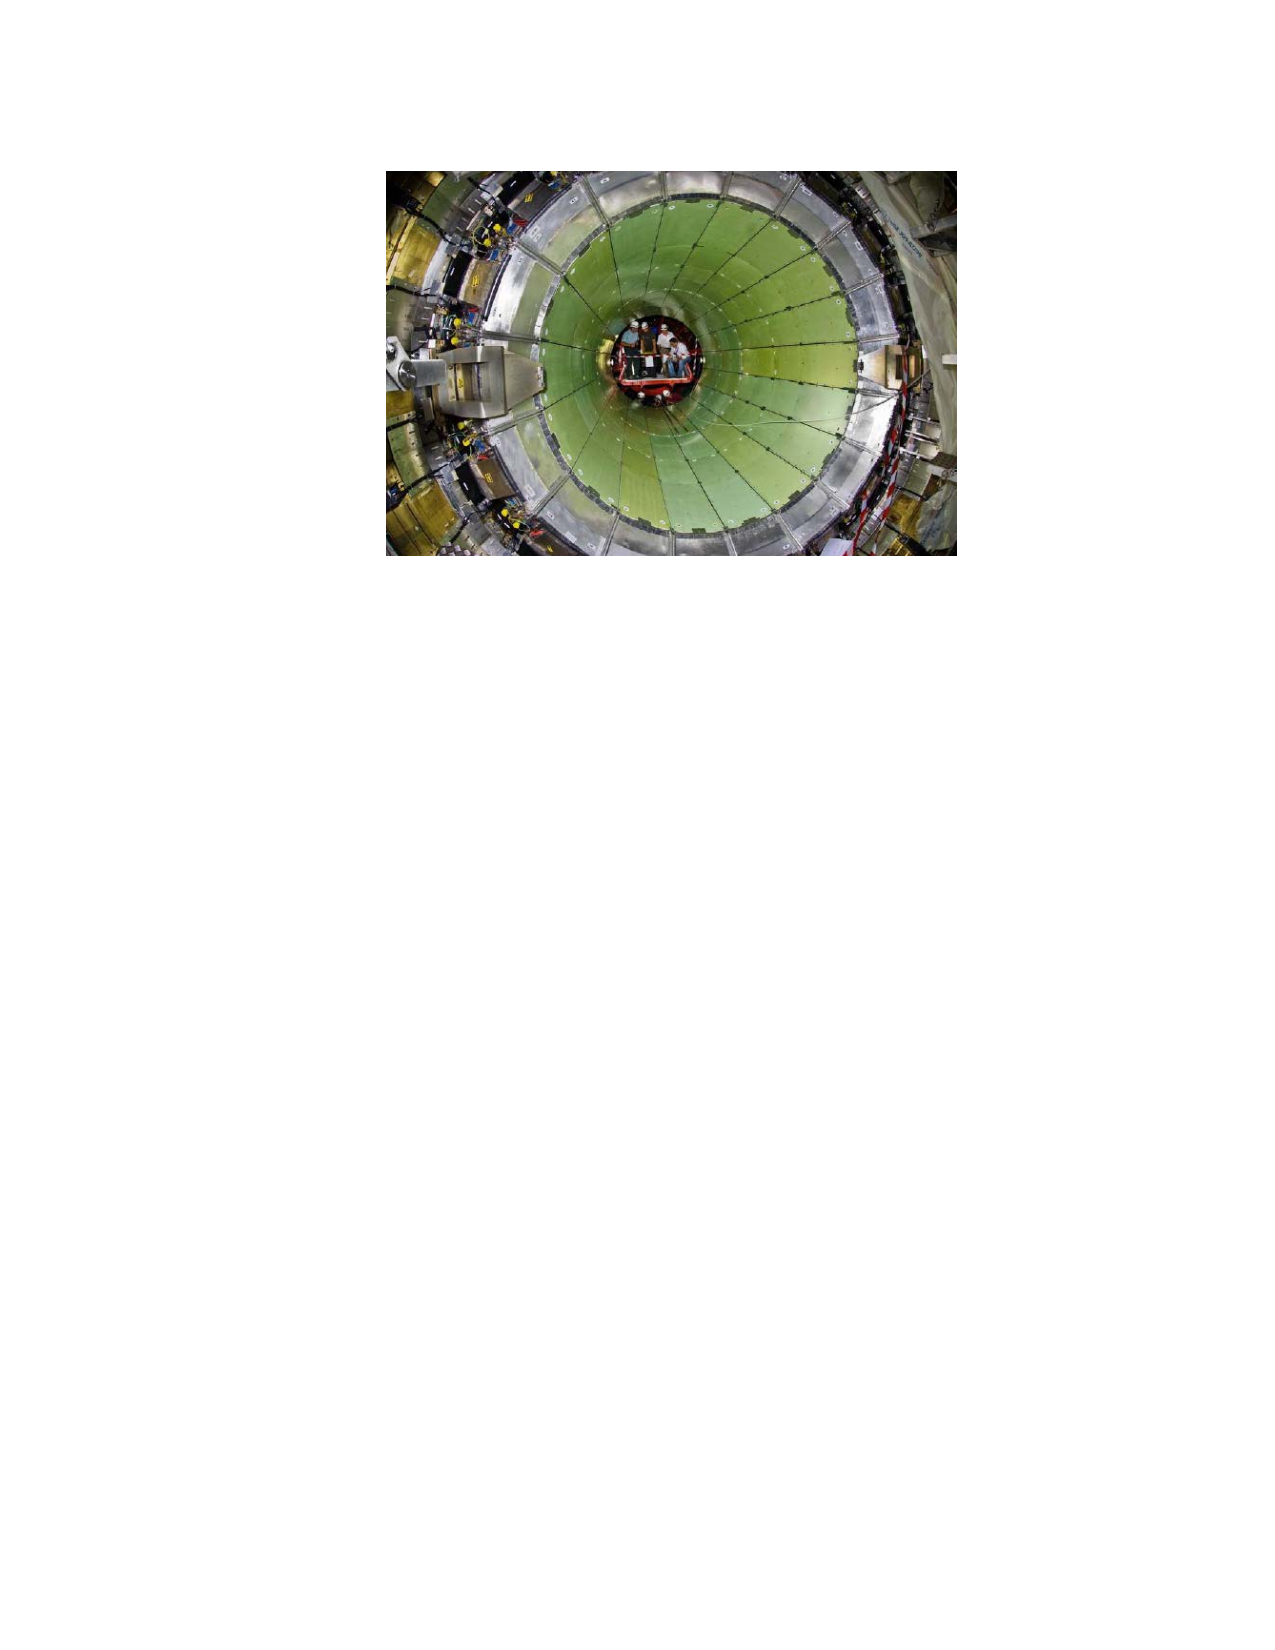
\includegraphics[width=.45\textwidth]{pics/ecal_barrel}
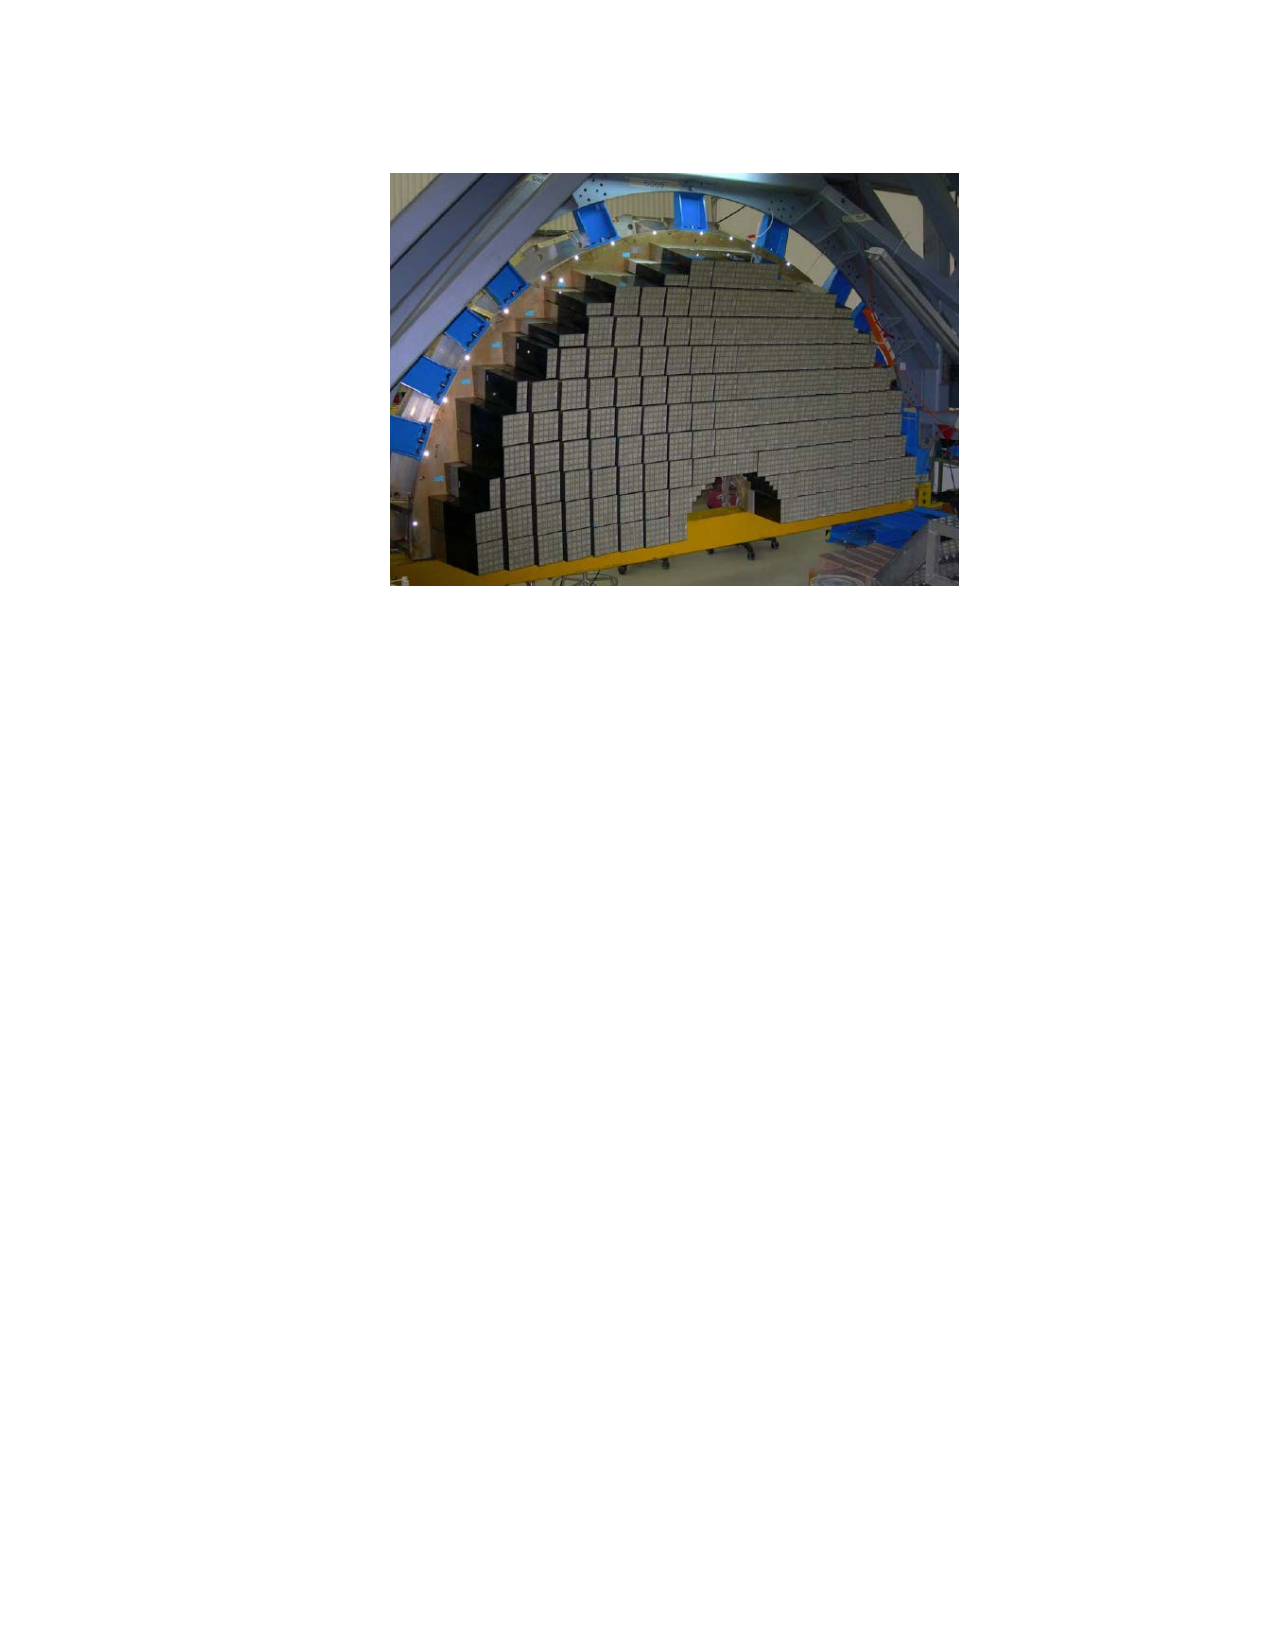
\includegraphics[width=.45\textwidth]{pics/ecal_dee}
\end{center}
\caption{(left) The ECAL barrel installed within CMS. (right) A single dee of the ECAL endcap.}
\label{fig:ecal_photos}
\end{figure}

The ECAL consists of 75,848 Lead Tungstate PbWO$_4$ scintillating crystals (Figure \ref{fig:ecal_crystal}). 
The ECAL is separated into two sections: the endcaps and the barrel. 
The Barrel consists of 61200 $2 \times 2 \times 23$ cm crystals, separated into 36 supermodules,
  and is contained in $|\eta| < 1.48$. The endcaps are separated into 4 dees (Figure \ref{fig:ecal_photos})
 of 3662 crystals with each crystal measuring $3 \times 3 \times 22$ cm. 
The 4 dees cover a  pseudorapidity range between $1.48 < |\eta| < 3.0$.
The endcaps are behind a preshower detector, composed of two lead absorbers 
interleaved with silicon detectors. The preshower covers the pseudorapditiy range
of $1.653 < |\eta| < 2.6$ with each silicon sensor covering a square are of 
63 mm $\times$ 63 mm divided into 32 strips. The preshower is designed to give significantly
better spatial resolution than using the endcap alone to aid in the separating single photons
and $\pi^0 \rightarrow \gamma\gamma$ decays used to calibrate the endcap. As the first layer is
2 radiation wavelengths thick, such that the majority of incident single photons will  
begin to shower before reaching the second layer.  The conversion of the photons by the preshower 
assists in distinguishing directly produced photons from pairs
of photons resulting from neutral pion decays. 

The light in each crystal is collected as a current 
and amplified by avalanche photodiodes (APDs) in the barrel
region and vacuum phototriodes (VPTs) in the endcap. This transition is
necessary as the endcap region must be tolerant to much
higher levels of radiation damage from softly scattered (low momentum transfer $Q^2$)
interactions. 
\begin{figure}
\begin{center}
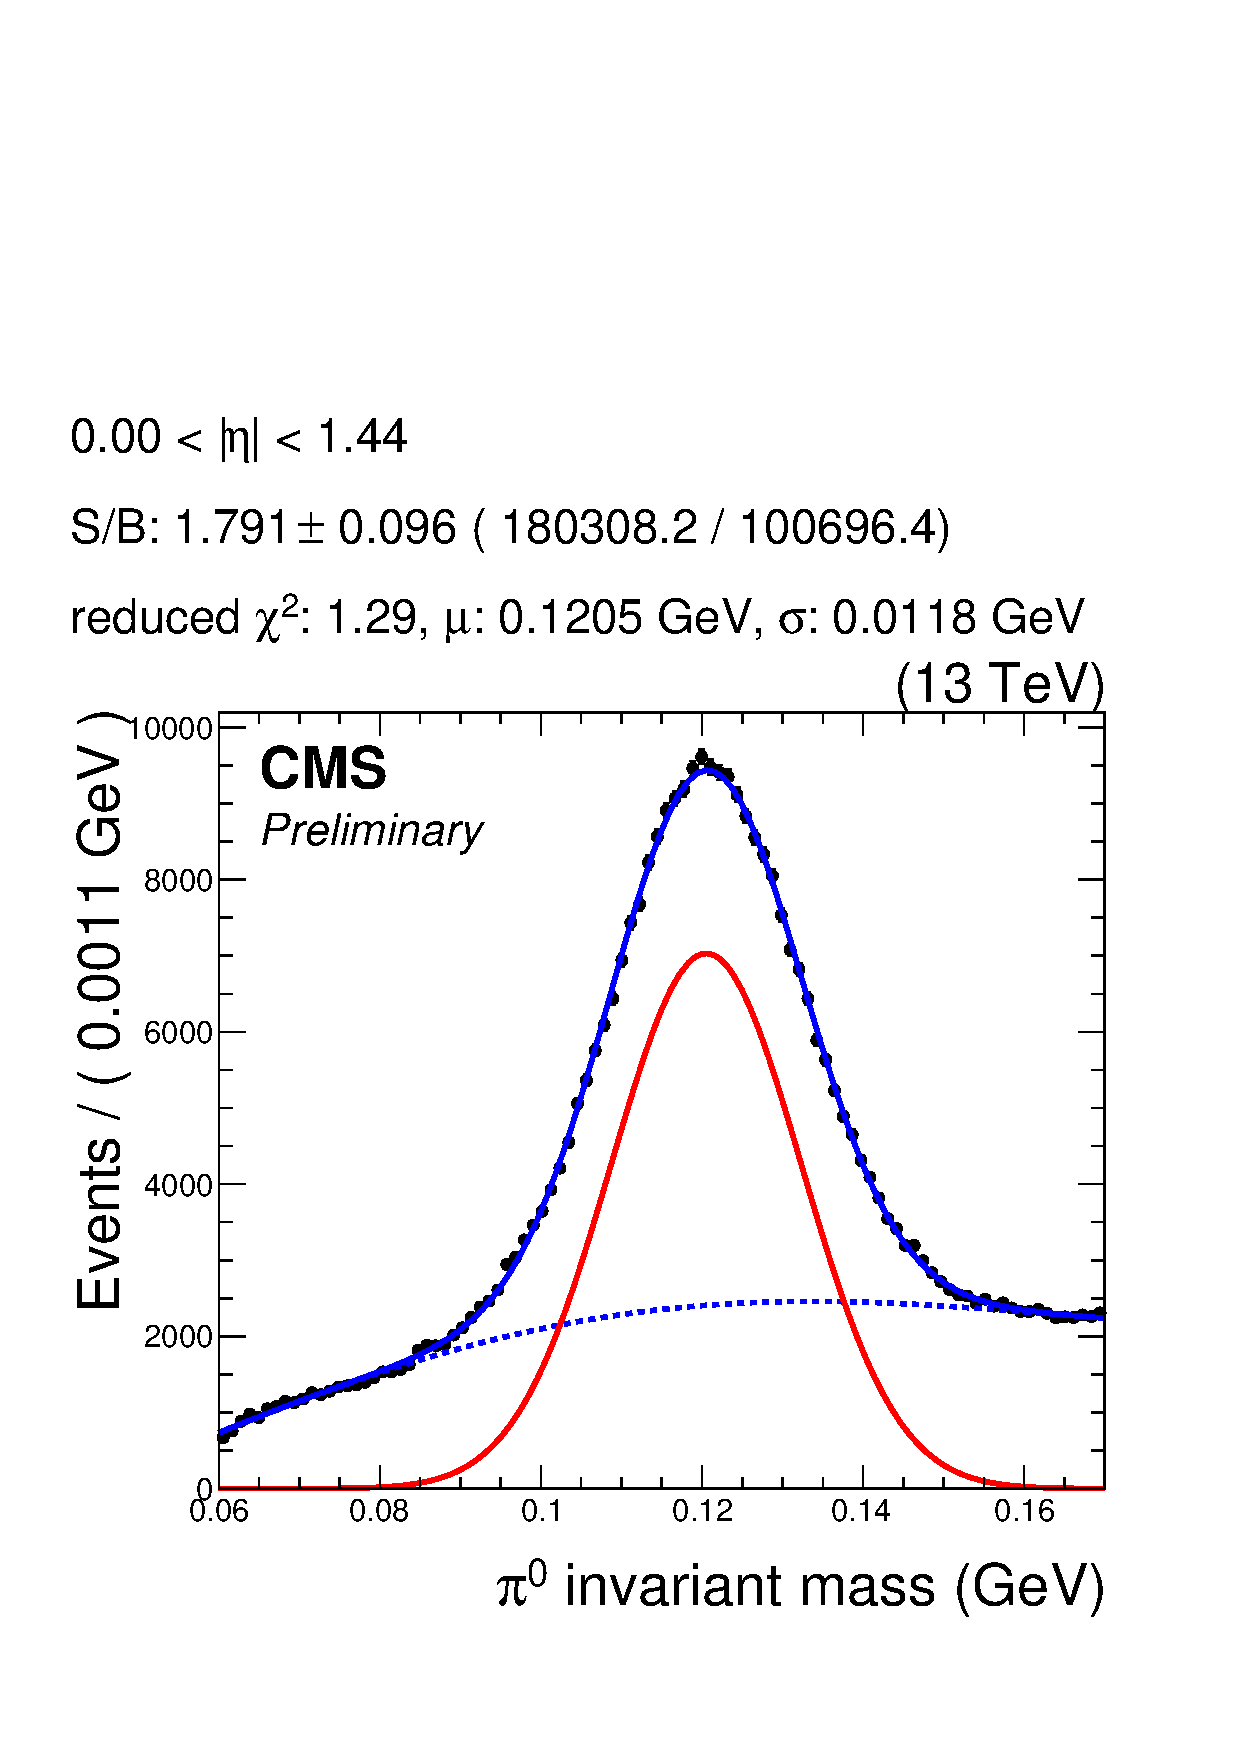
\includegraphics[width=.45\textwidth]{pics/pizero_eb}
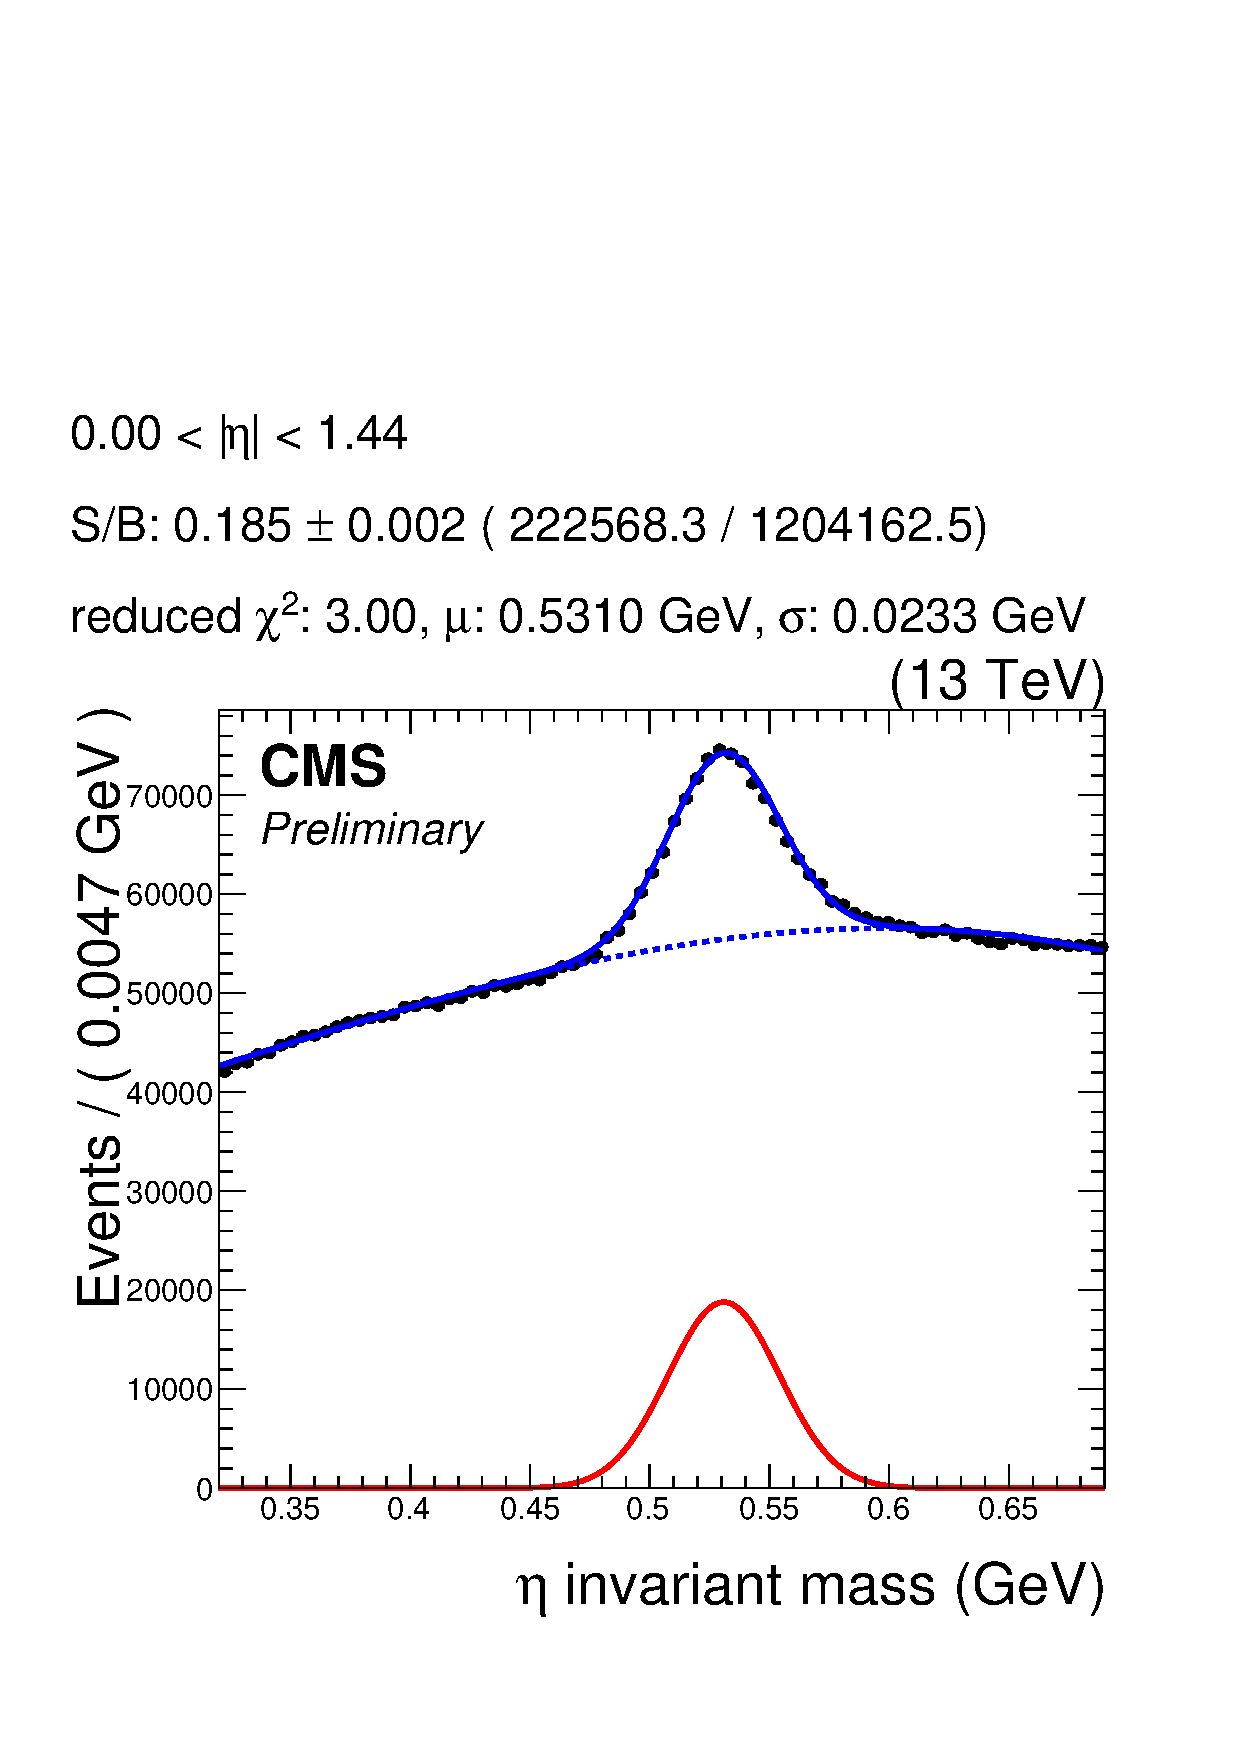
\includegraphics[width=.45\textwidth]{pics/eta_eb_2015b}
\end{center}
\caption{Calibration data for used for the pizero and eta calibration of the ECAL}
\label{fig:pizero_eta}
\end{figure}
The detector is calibrated with a method that reconstructs the mass of neutral
pion and eta mesons to precisely calibrate the entire ECAL (Figure \ref{fig:pizero_eta}). 
The copious production of these particles in hadronic jets at the LHC allows us to
perform this calibration rapidly, even at very low luminosity. 

Under irradiation, the crystals undergo transparency changes 
due to the formation of color centers, which interestingly recover spontaneously when there
is no radiation present. As the crystal transparency affects the energy measurement,
the crystal transparency is continuously monitored by a laser monitoring system. 
The system takes advantage of a 3 $\mu$s gap in the LHC bunch train to inject the
pulses at a rate of 100 Hz. This rate allows for a measurement of every crystal
to be made at least every 30 minutes. In the barrel, only laser
 pulses of known wavelength are injected through optical fibers. In the endcap, LEDs provide
an additional wavelength. 

\section{Hadronic Calorimeter (HCAL)}

\begin{figure}
\begin{center}
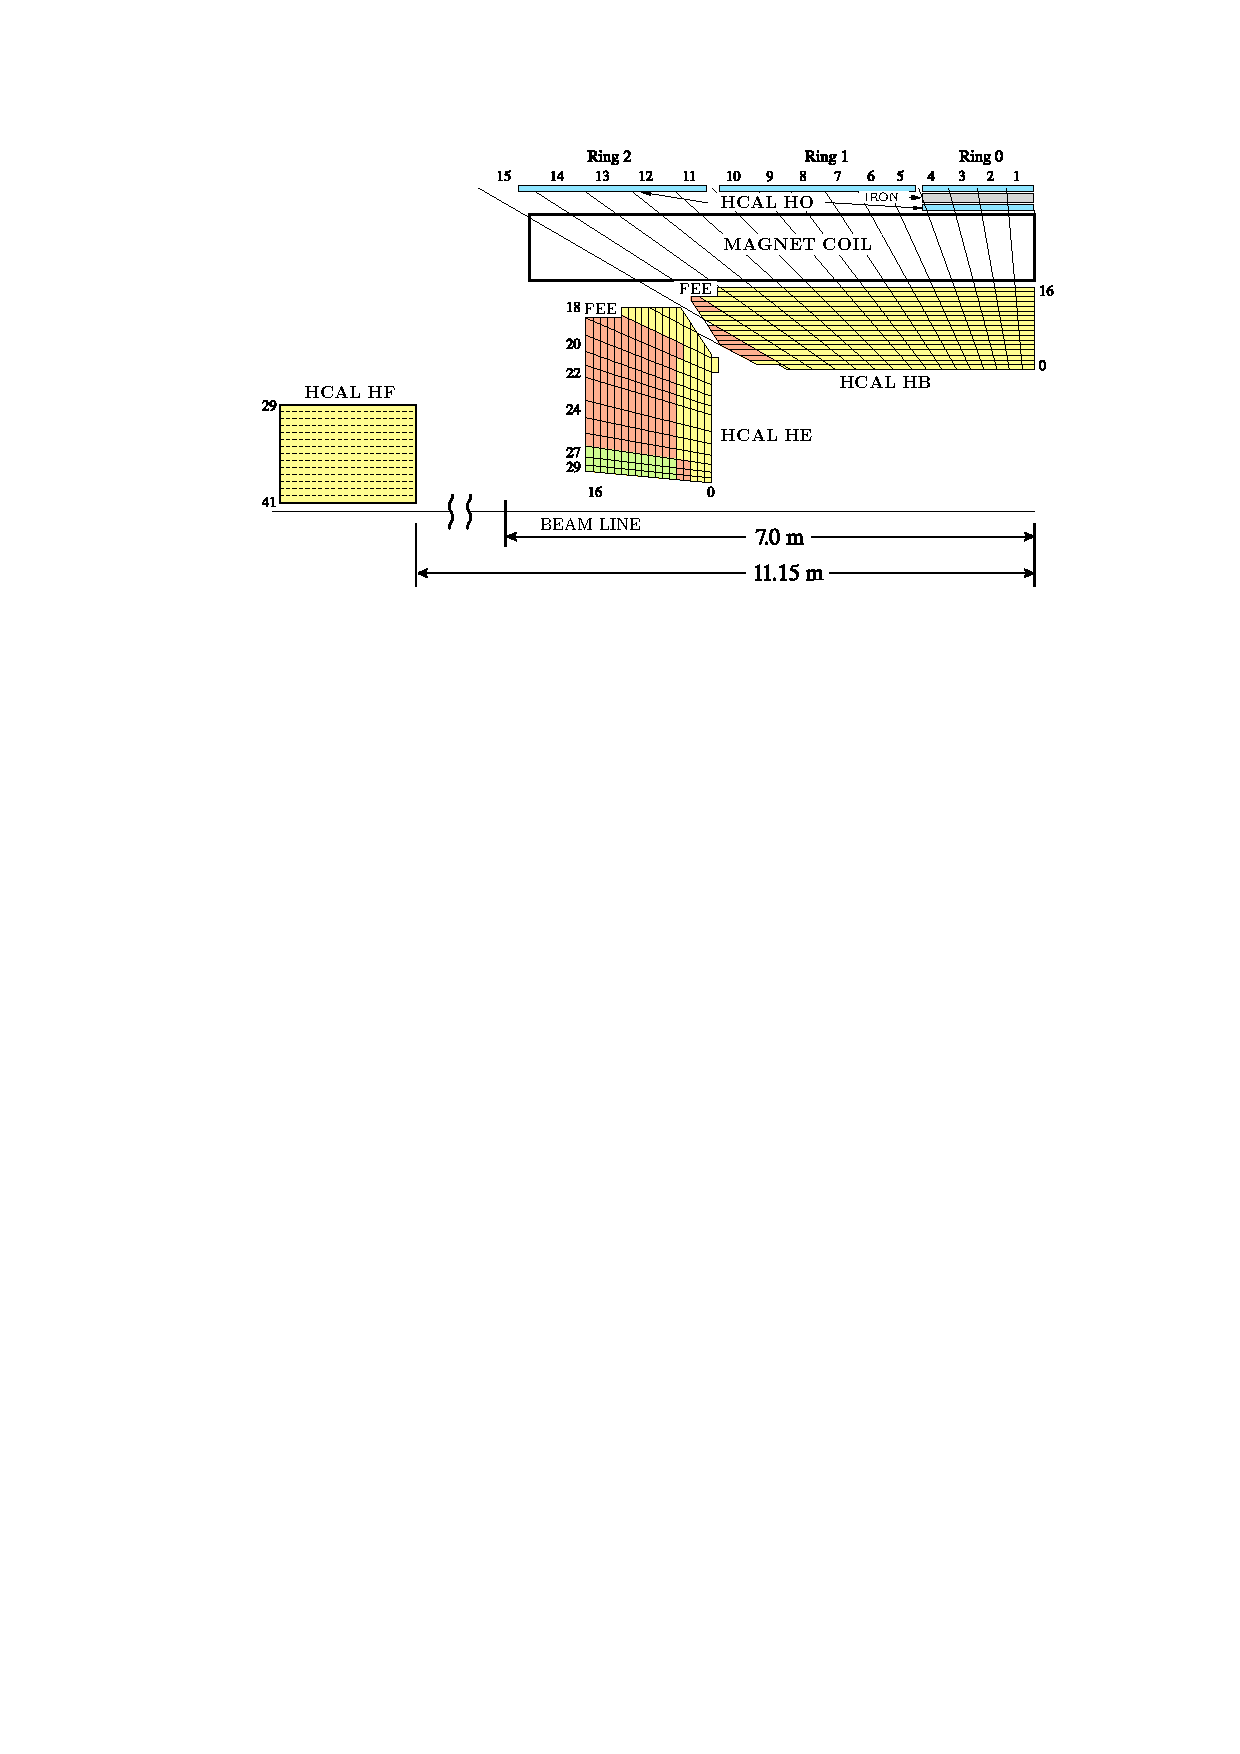
\includegraphics[width=.95\textwidth]{pics/hcal_diagram}
\end{center}
\caption{Kinematic acceptance of the CMS HCAL.}
\label{fig:hcal_diagram}
\end{figure}

\begin{figure}
\begin{center}
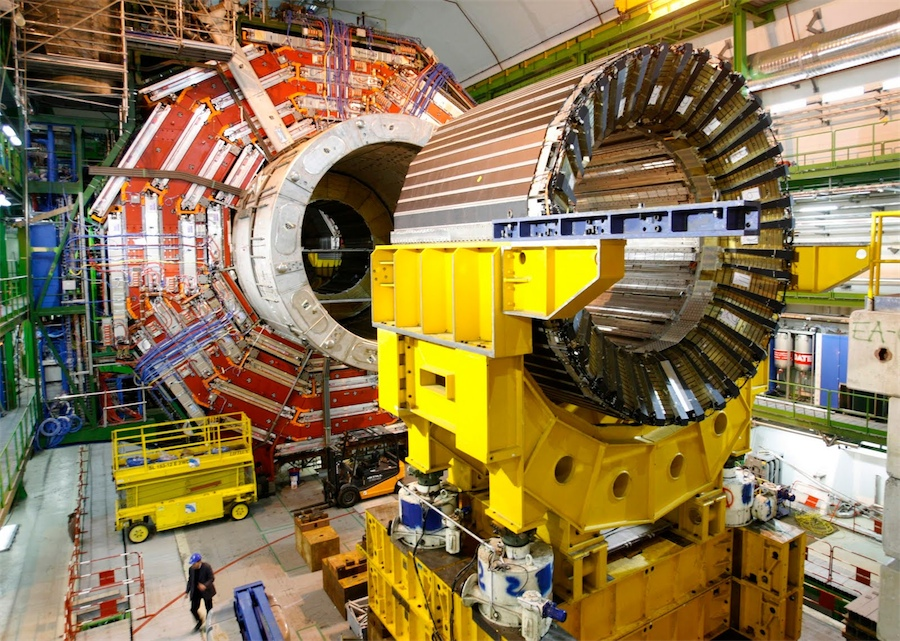
\includegraphics[width=.65\textwidth]{pics/naked_hcal}
\end{center}
\caption{The CMS HCAL outside of the CMS detector.}
\label{fig:hcal_naked}
\end{figure}
Surrounding the ECAL. The Hadronic Calorimeter (HCAL) is hermetic (full coverage of interaction), non-compensating (asymmetric electromagnetic and hadronic energy response), sampling calorimeter (showering material differs from measurement material) designed to measure the the energy of neutral hadrons which would not deposit significant energy in the ECAL. 
%%  The ratio of energy between the two detectors for defined solid angle, $H/E$, is a 
%% commonly used particle identification criterion. 

The HCAL consists of 9072 channels divided between four sections: the barrel (HB), the endcaps (HE), 
two forward calorimeters (HF) and an outer hadron calorimeter (HO). The barrel
 and endcap of the HCAL cover $|\eta| < 4$. The forward detectors extend the sub-detector's reach to $|\eta| =5$. 
As the HCAL is radially limited by the design of the enclosing solenoid, 
the HO is built around the solenoid to measure any leaked energy from high momentum showers. 
The towers are segmented into towers that project into $\eta,\phi$ space with
 $\Delta \eta \times\Delta \phi= 0.087 \times 0.087$ for $|\eta| < 1.6$ and 
$\Delta \eta \times\Delta \phi= 0.17 \times 0.17$ for $|\eta| > 1.6$. 

The HF sub-detector is a Cherenkov light detector using quartz fibers within 165 cm of steel absorber. 
Photomultiplier tubes (PMTs) connected to the fibers convert the detected light into an electronic signal.
 Cherenkov detectors utilize the characteristic electromagnetic ``sonic boom'' created by particles traveling
 faster than light can travel in a material. As the angle of emission and intensity of the
 radiation depends on the velocity of the particle. For energetic
particles $E>1$ GeV the energy lost to the radiation is negligible \cite{detectorbook}.

Unlike electromagnetic showers, hadronic interaction cross sections are an order of magnitude smaller for the same material. To compensate cost effectively, hadronic calorimeters are constructed from dense materials 
such as copper, iron, lead, uranium, and tungsten \cite{tully}. In general, hadronic showers
produce irregularly shaped deposits and varied particle content when compared to electromagnetic showers. 
 
\begin{figure}
\begin{center}
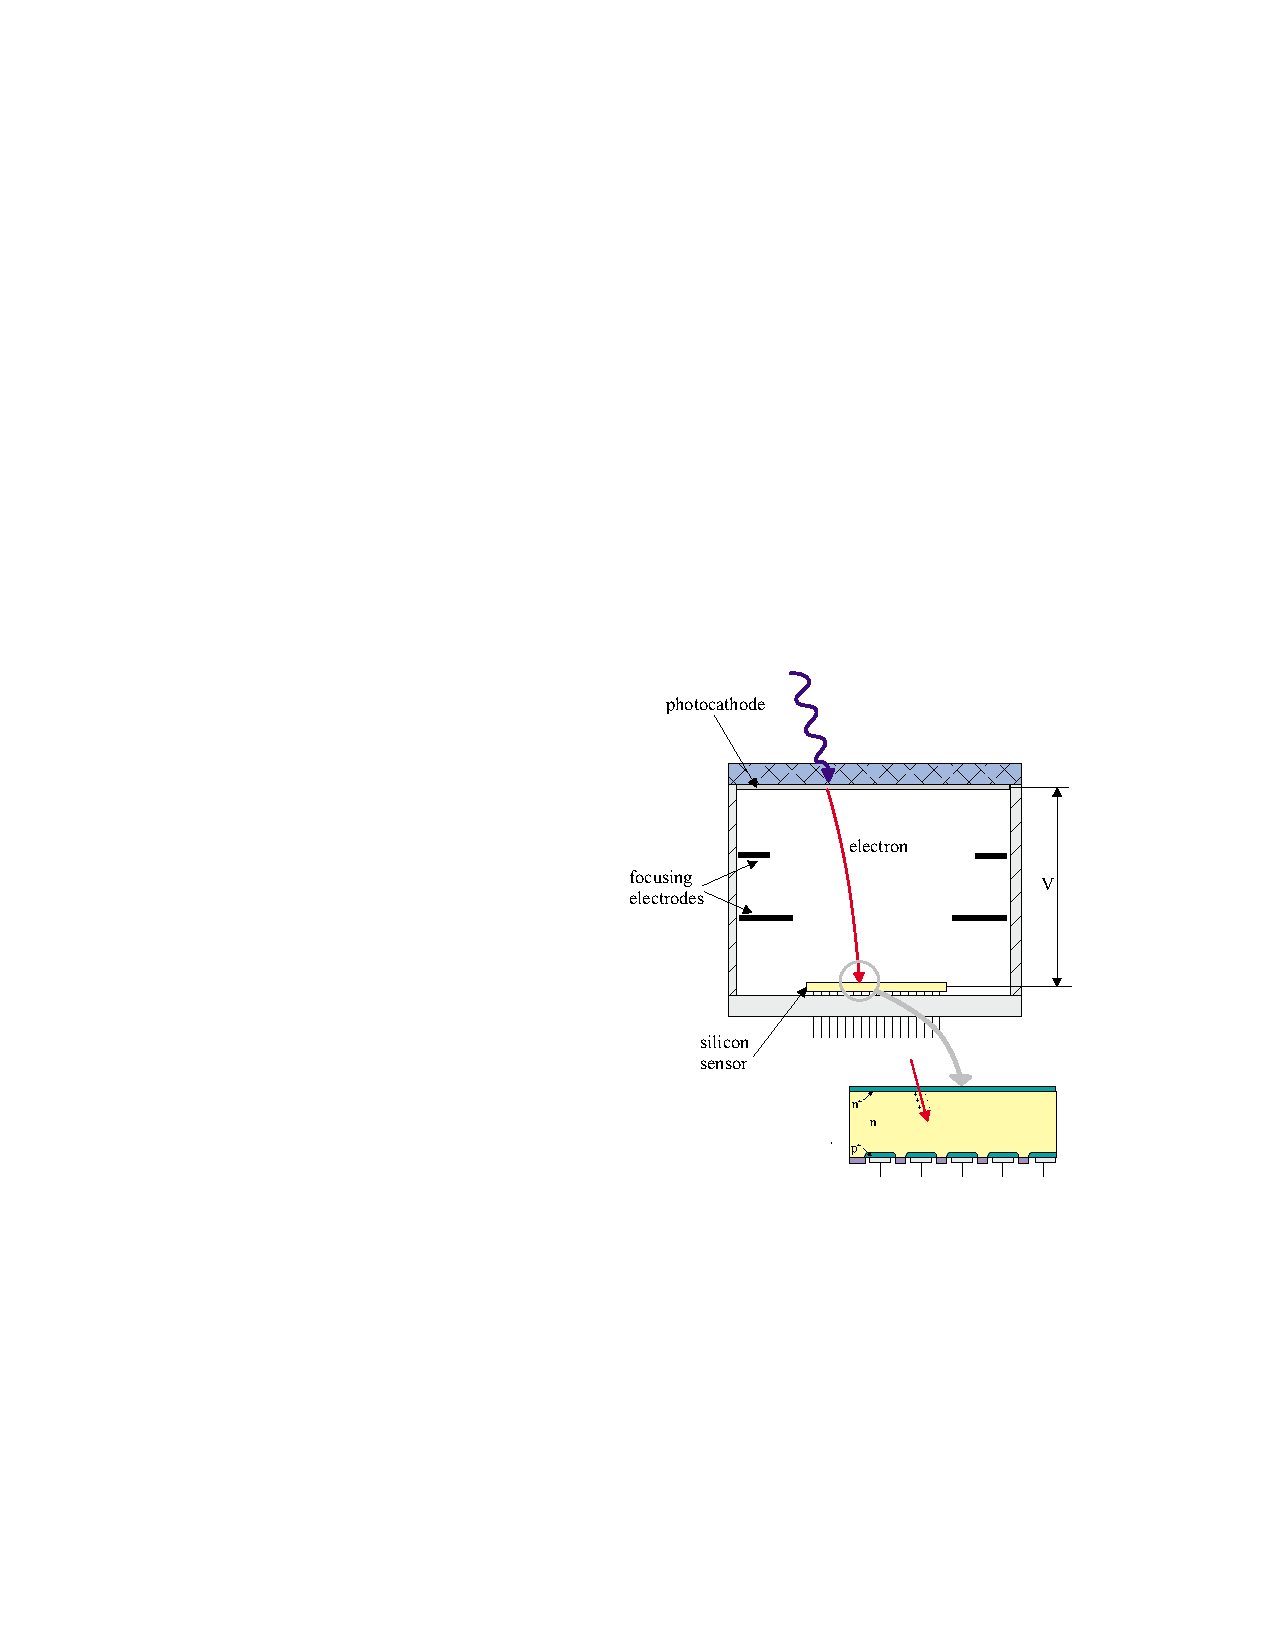
\includegraphics[width=.45\textwidth]{pics/HPD}
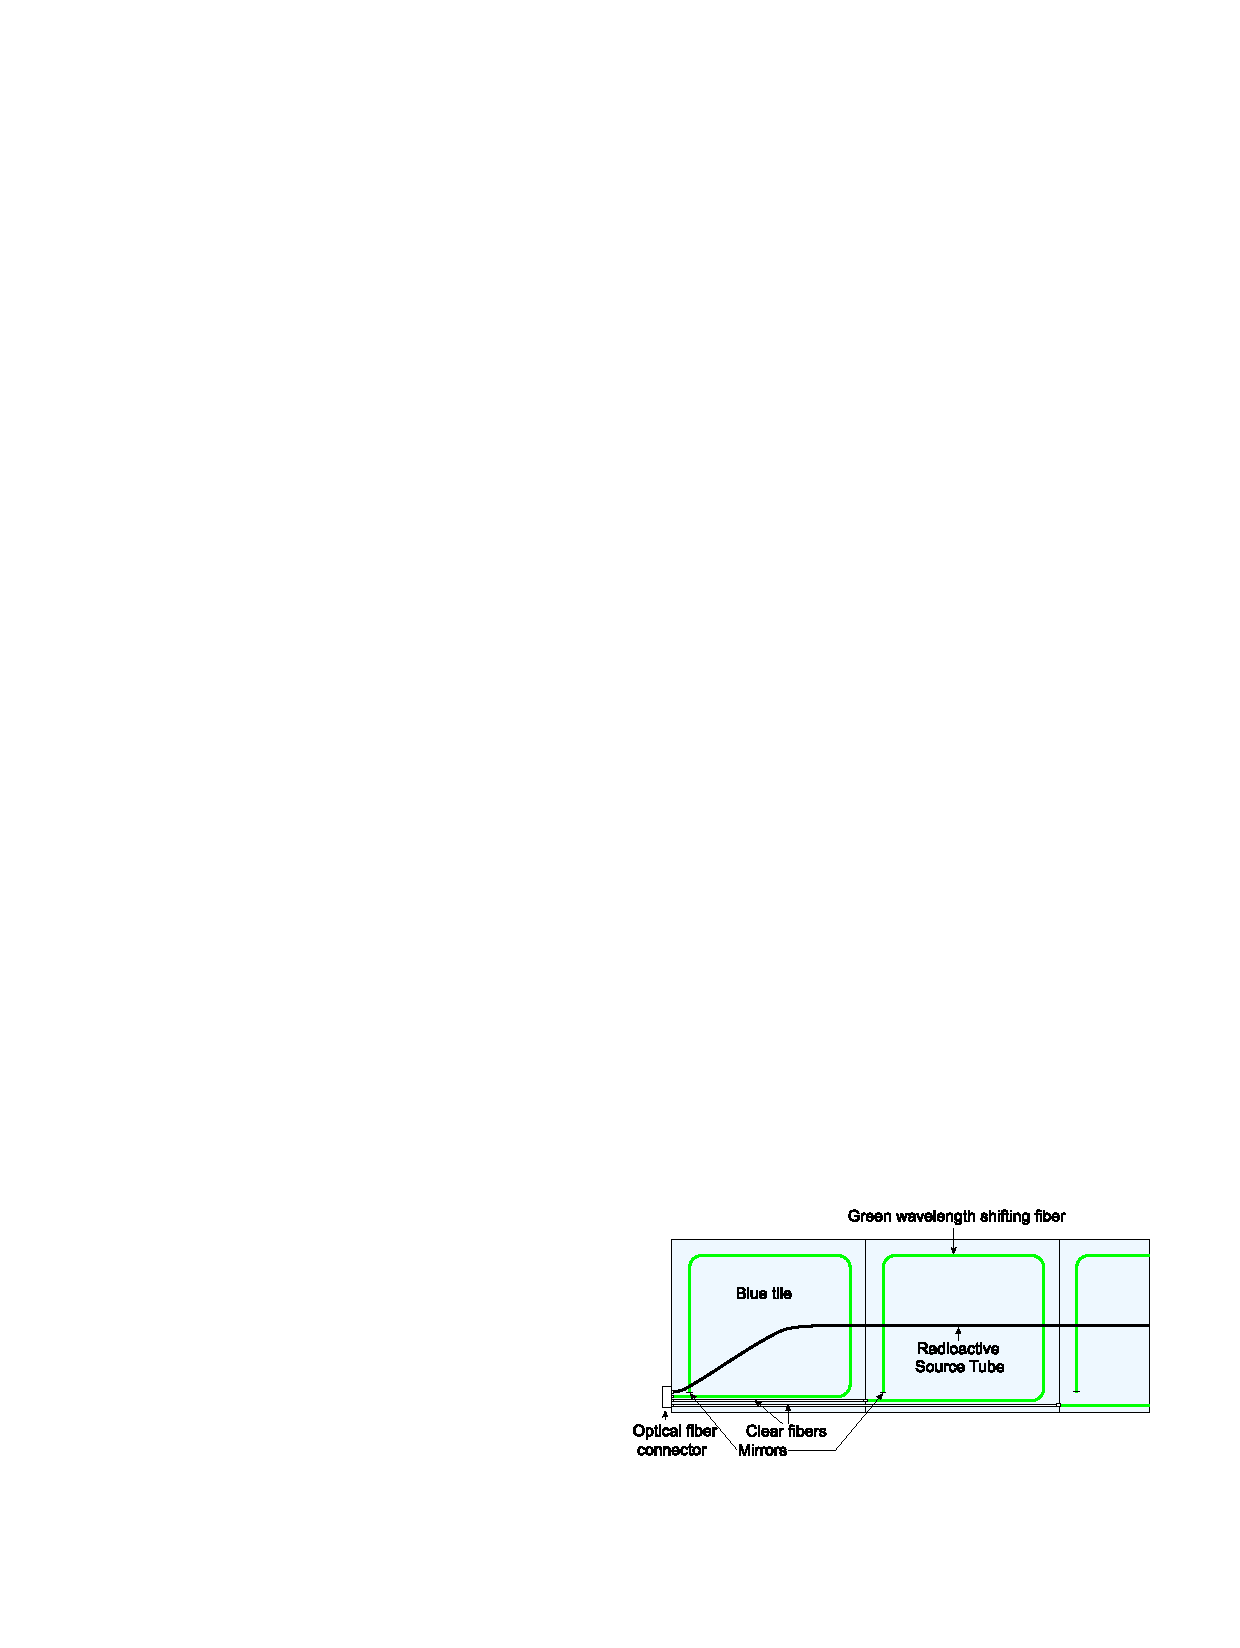
\includegraphics[width=.45\textwidth]{pics/HCALfiber}
\end{center}
\caption{(left) A diagram of a typical HPD under a potential difference $V$ \cite{hpd}. (right) 2 visible
 scintillator plates of 16 within a megatile \cite{hcalcalib}.}
\label{fig:hpd_fiber}
\end{figure}

\begin{figure}
\begin{center}
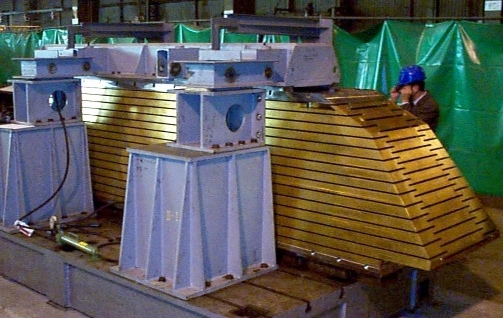
\includegraphics[width=.45\textwidth]{pics/hb_wedge}
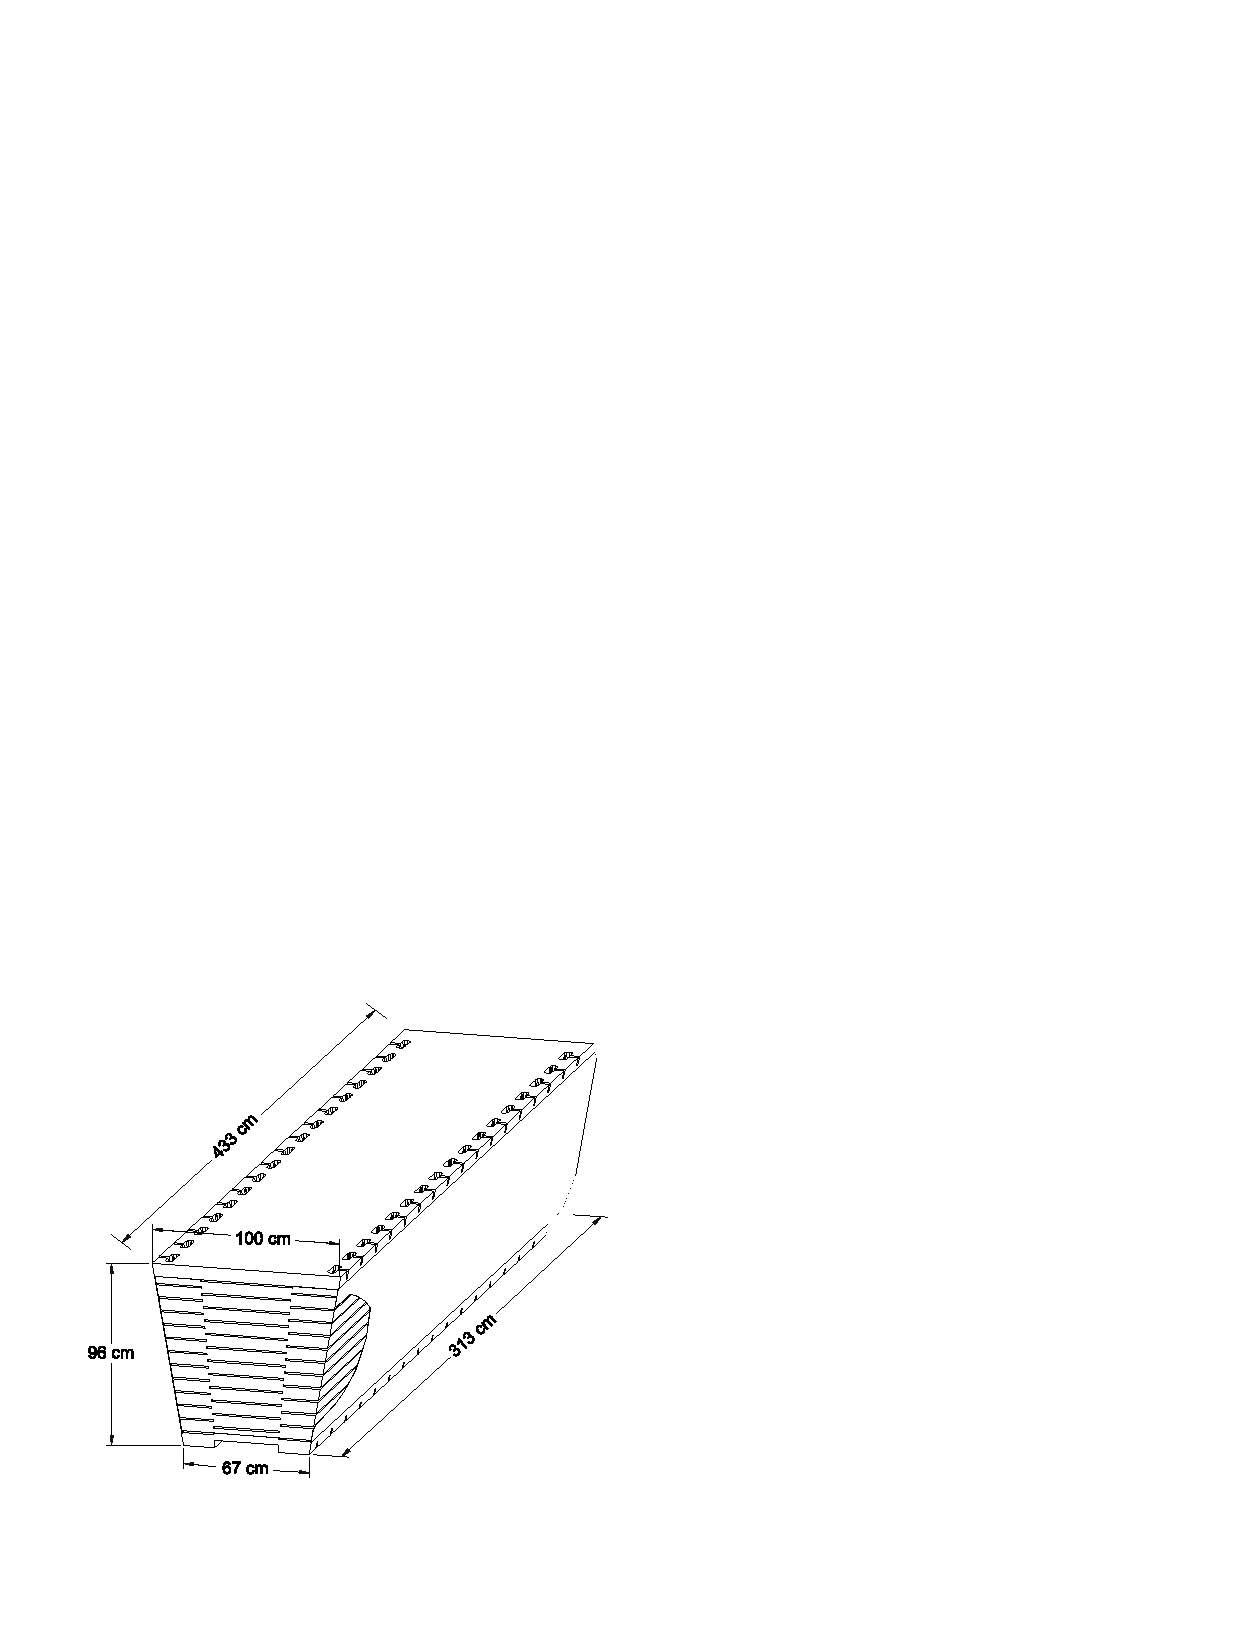
\includegraphics[width=.45\textwidth]{pics/HBwedge}
\end{center}
\caption{(left) A single wedge of the CMS HCAL barrel. (right) Scintillator trays (Figure \ref{fig:hpd_fiber}) are inserted into 
slots at the end of the wedge \cite{hcalcalib}.}
\label{fig:hb_wedge}
\end{figure}

The HB/HE are constructed as alternating layers of brass absorber and plastic scintillator. 
The light is merged, wavelength shifted and measured by hybrid photodiodes (HPDs) with 17 channels per HPD. The HPD
(Figure \ref{fig:hpd_fiber}) functions by converting light into photoelectrons emitted at the photocathode and accelerated
by a potential difference of 8-10 kV toward the silicon layer. The absorbed energy in the silicon sensor creates 
electron hole pairs which induce a detectable current. The light is wavelength shifted to avoid a loss of photons 
when piping light to the HPDs through a small cross sectional fiber.
%%  Wavelength shifting can seemingly evade phase
%% space conservation (photon flux per unit area) by redefining the phase space element in a lower energy wavelength
%% spectrum.

Large deposits of energy reconstructed of hadronic energy in the HCAL are of particular interest 
to the study of long lived decays when the long-lived decay occurs inside of the HCAL calorimetry. Although 
not studied in this thesis, large signal to background discrimination can be found by
 requiring a calorimeter deposit to have no
associated tracks and a large ratio of hadronic energy $H/E$. It is also of concern that 
the HCAL is known to have spurious noise that generally results in the mis-measurement 
of missing energy, and mimics the signature of long lived decay signatures. It is possible
that using a coincidence of activity in the muon spectrometer could suppressed these events.  

\section{Tracking Layers}

\begin{figure}
\begin{center}
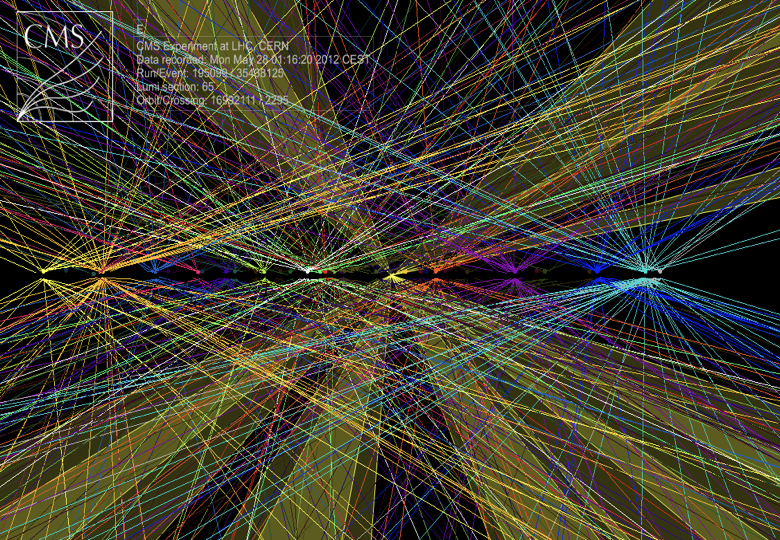
\includegraphics[width=.75\textwidth]{pics/pileup_vertices}
\end{center}
\caption{Pileup interactions during a single bunch crossing in data.}
\label{fig:pileup}
\end{figure}

The CMS tracker's purpose is to reconstruct the trajectories (or simply ``tracks'') of the charged particles
 copiously produced in hadron collisions. For a silicon strip detector, like that in CMS, the position measurements are derived from the ionization charge in the strips known as a charge cluster. As photons and electrons exhibit nearly identical signatures in the ECAL, 
the reconstruction of the track associated with electron energy clusters
is the main component of their particle identification. Using knowledge of the magnetic field along the 
trajectory with position measurements taken from multiple layers of silicon strips and
 pixels, the helical tracks are fit and kinematic parameters extracted.  

By fitting trajectories to vertices, the tracker enables the reconstruction 
of the hard interaction position (Figure \ref{fig:pileup}). As only one vertex is typically
of interest, identifying background vertices and subtracting their contribution is of increasing
importance with the increasing number of pile up interactions. 

\begin{figure}
\begin{center}
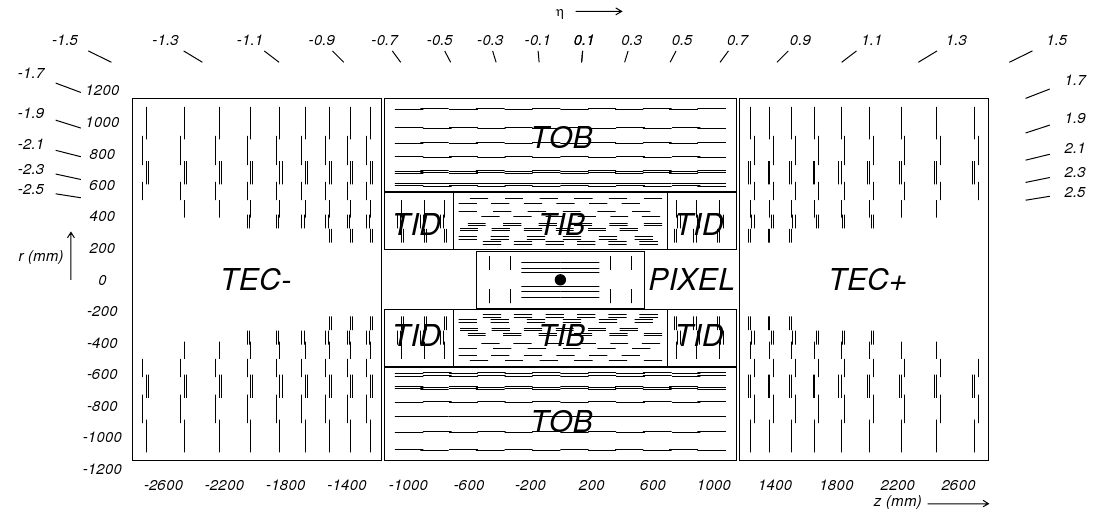
\includegraphics[width=.95\textwidth]{pics/tracker_diagram}
\end{center}
\caption{Kinematic acceptance of the CMS tracker.}
\label{fig:tracker_diagram}
\end{figure}

\begin{figure}
\begin{center}
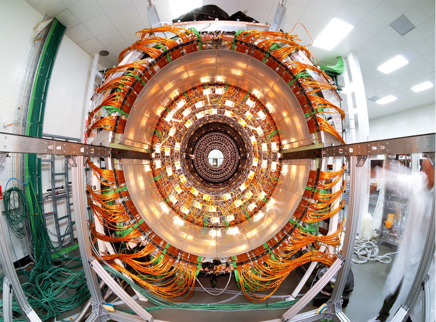
\includegraphics[width=.45\textwidth]{pics/naked_pixel}
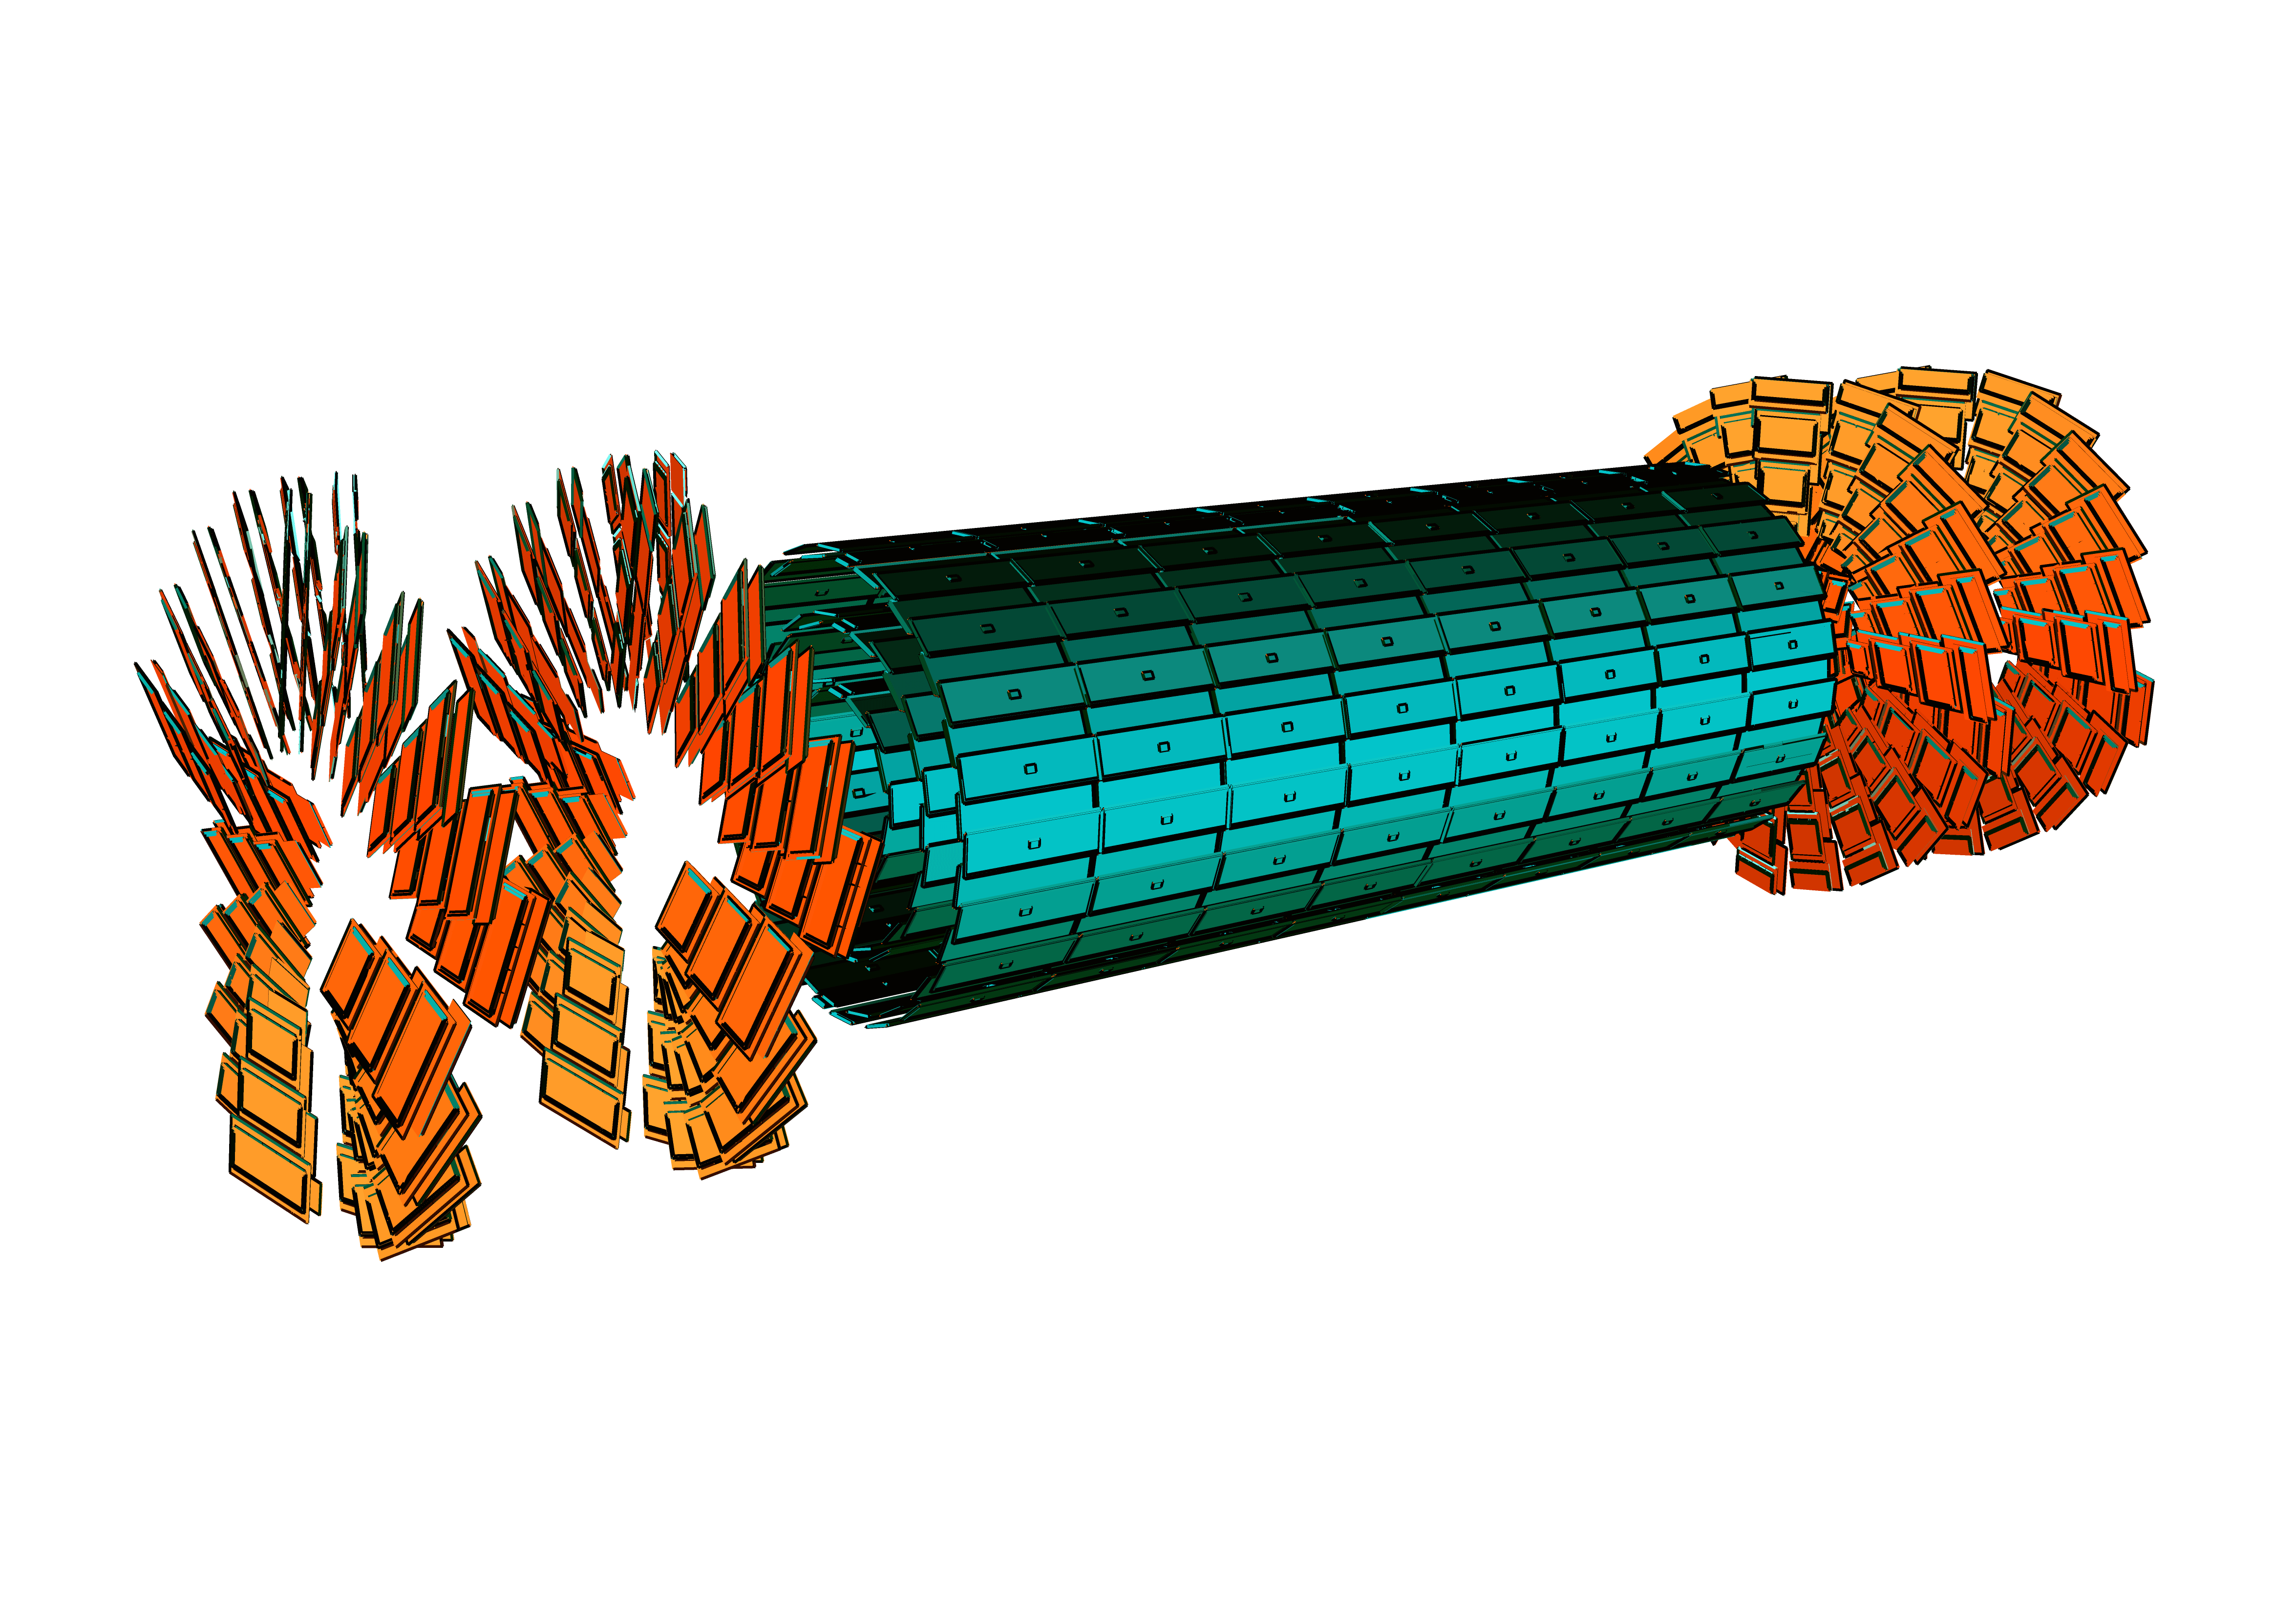
\includegraphics[width=.45\textwidth]{pics/pixel_diagram}
\end{center}
\caption{The two wheels and three layers of the CMS Pixel detector.}
\label{fig:pixel}
\end{figure}
\begin{figure}
\begin{center}
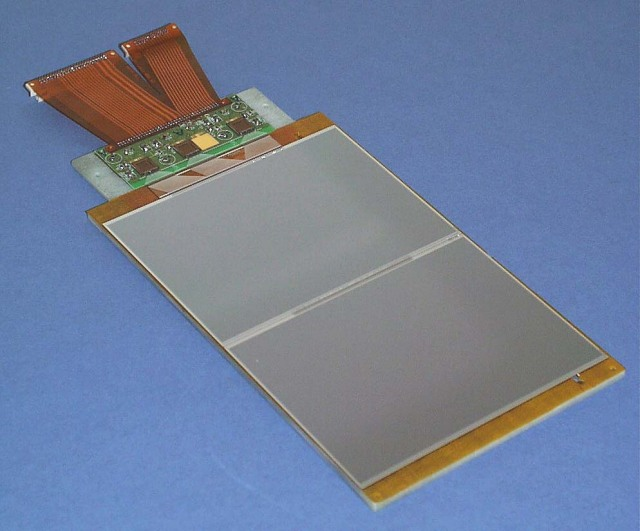
\includegraphics[width=.45\textwidth]{pics/tracker_module}
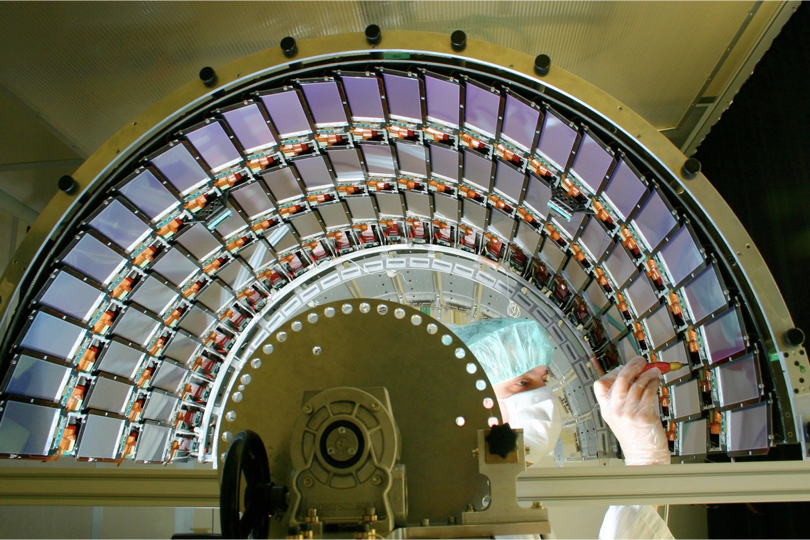
\includegraphics[width=.45\textwidth]{pics/tracker_strips}
\end{center}
\caption{(left) A single CMS tracker module. (right) A tracker inner barrel module.}
\label{fig:tracker_strips_and_module}
\end{figure}
The CMS tracker is the world's largest all silicon detector with a
sensitive area larger than 200 m$^{2}$ (Figure \ref{fig:tracker_strips_and_module}) \cite{TRK-11-001}. 
The tracker consists of 10 layers
in the barrel region: 4 inner barrel layers (TIB) and 6 outer barrel layers (TOB). The endcap is made up of 
12 disks: 3 inner disks (TID) and 9 endcap disks (TEC). The CMS pixel detector (Figure \ref{fig:pixel}) 
consists of three layers are radii of 5.3 cm, 7.2 cm and 11 cm
and 2 disks on each size of the barrel at 34.6 and 46.6 cm from the either side of the interaction point. 

Track reconstruction resolution is affected by a series of kinematic dependent effects. 
Track reconstruction is degraded by interactions with the tracker material. With some finite probability
as a function of the material density and thickness, the track will randomly scatter. The overall rate of this
 scattering degrades overall tracking resolution. 
High energy charged particles for which the detector volume and strength of the magnetic field do not
permit the track to bend cause significant degradation of momentum resolution as well 
as charge sign determination. For low energy tracks $\sim$500 MeV, the strong magnetic field
deflects the charge particle into closed loops (loopers) within the tracker volume. 
As these tracks do not reach the calorimetry, they have no associated calorimeter deposit and 
are rarely considered in a non-specific analysis.

A track in a uniform magnetic field, like that of the CMS Solenoid
are parameterized by 5 parameters:
\begin{itemize}
\item $d_{\rho}$: the distance of closest approach to the reference point
\item $\phi_0$: azimuthal angle specifying the reference point to the helix center 
\item  $p_t^*$: charged signed transverse momentum
\item  $d_z$: signed distance of the helix from the reference point in the z direction
\item $\tan \lambda$: the slope of the track 
\end{itemize}
using these parameters, the trajectory is parameterized in the turning angle $\phi$:
\begin{align*}
x =& x_0 + d_\rho \cos \phi_0 + \alpha p_{t}^* ( \cos \phi_0 - \cos(\phi_0 + \phi) ) \\
y =& y_0 + d_\rho \sin \phi_0 + \alpha p_{t}^* ( \sin \phi_0 - \sin(\phi_0 + \phi) ) \\
z =& z_0 + d_z - \alpha p_{t}^*  \tan \lambda \cdot \phi 
\end{align*}
In the context of displaced tracks, it is important to know that tracks do not necessarily 
have the same reference point. For CMS, each
individual track parameter is computed against a reference point determined by the the closest
point of approach to the beam line. For prompt physics, this reference point coincides with the
collision vertex used to compute the kinematic parameters for calorimeter jets. In contrast, when
tracks are displaced, the reference point used for the track is not the same as the reference point
for the calorimeter jet $\eta$ and $\phi$. This mis-match of coordinate systems affects the ultimate
track and jet association. 

\section{Muon Spectrometer}

\begin{figure}
\begin{center}
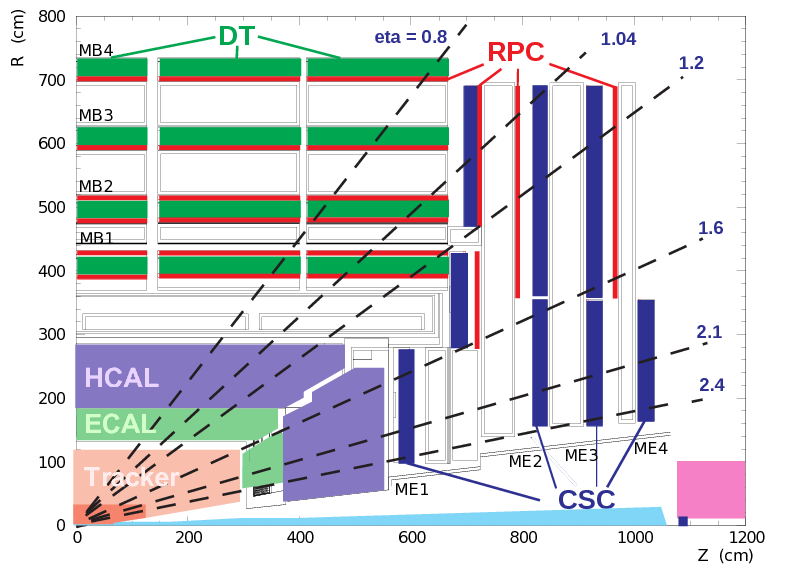
\includegraphics[width=.85\textwidth]{pics/muon_diagram}
\end{center}
\caption{Kinematic acceptance of the CMS Muon system.}
\label{fig:muon_diagram}
\end{figure}

\begin{figure}
\begin{center}
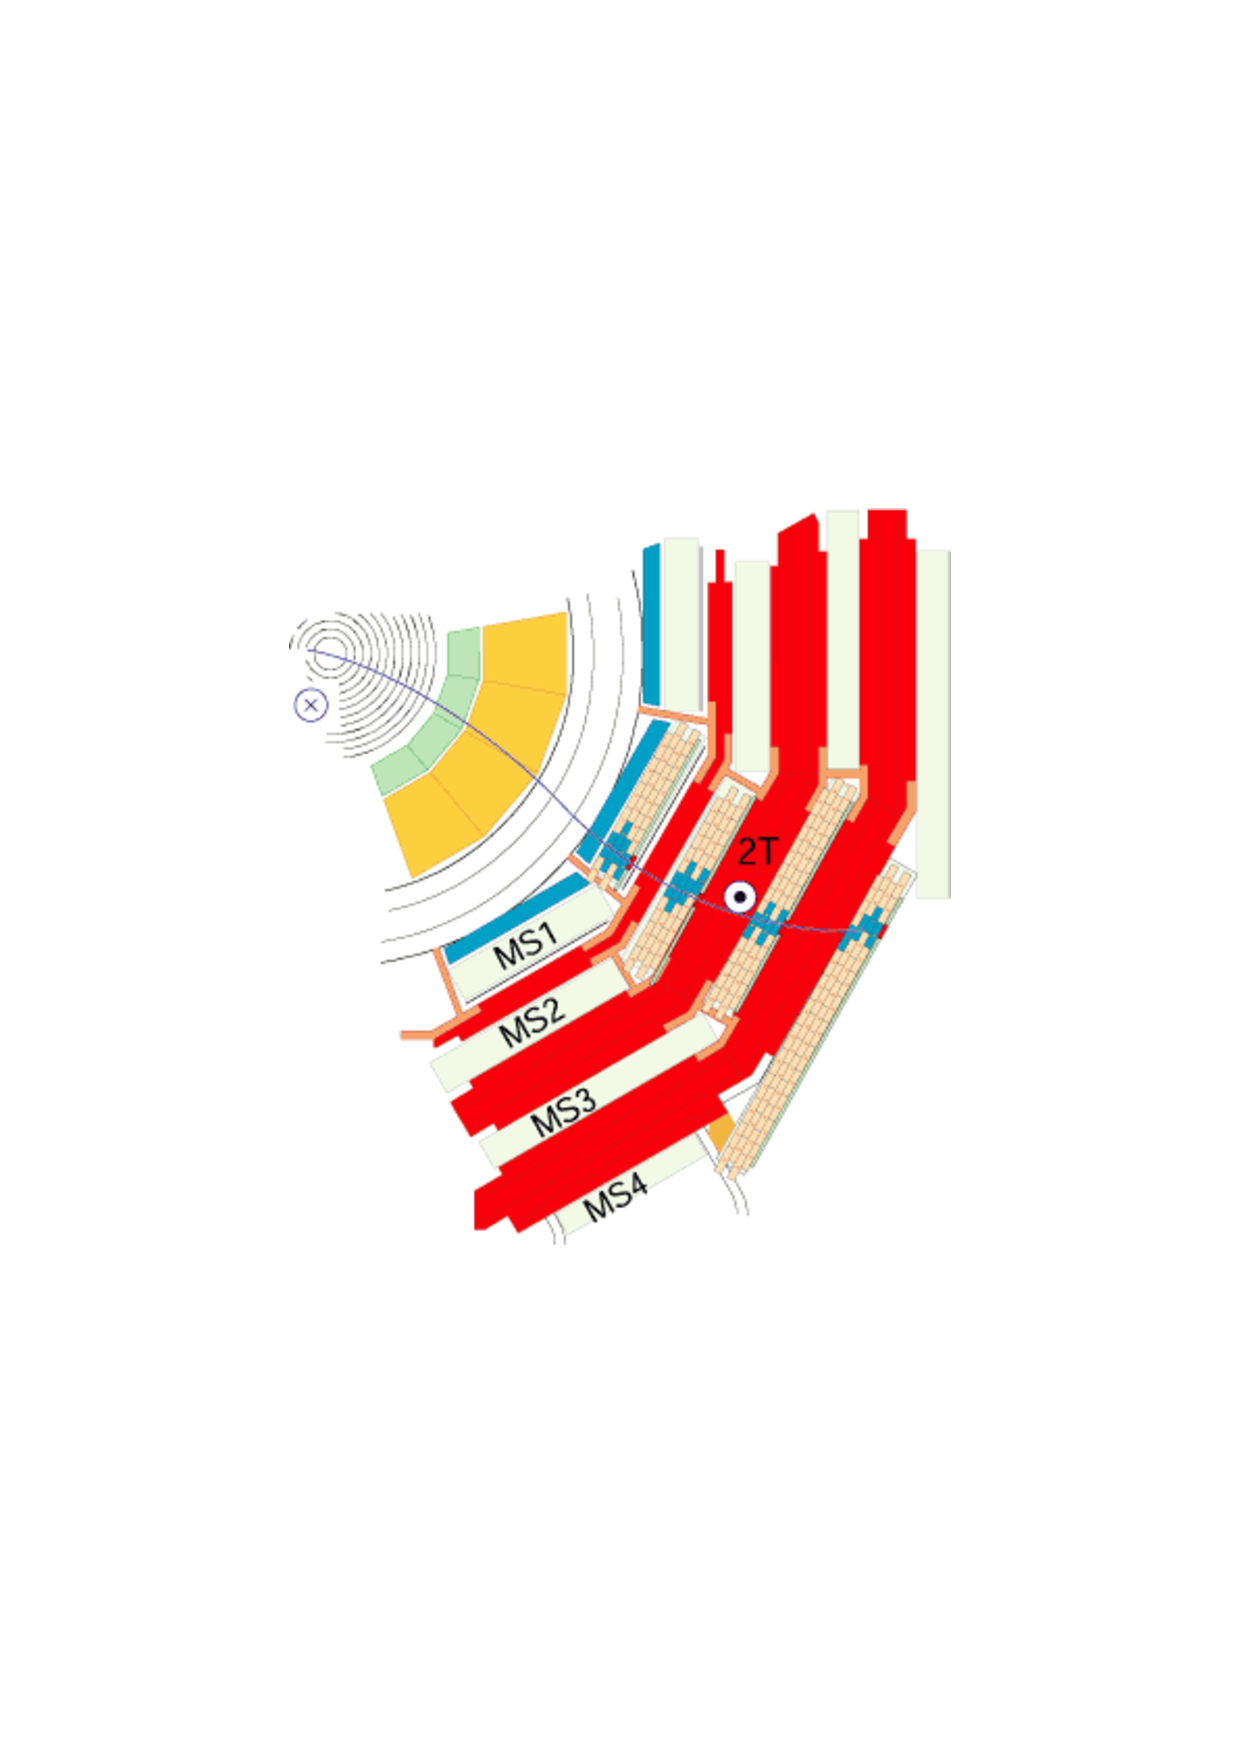
\includegraphics[width=.45\textwidth]{pics/muon_slice}

\includegraphics[width=.45\textwidth]{pics/cms_logo}
\end{center}
\caption{(left) A transverse slice of the muon detector. (right) The CMS logo depicting the change muon 
curvature outside of the solenoid.}
\label{fig:muon_slice}
\end{figure}

\begin{figure}
\begin{center}
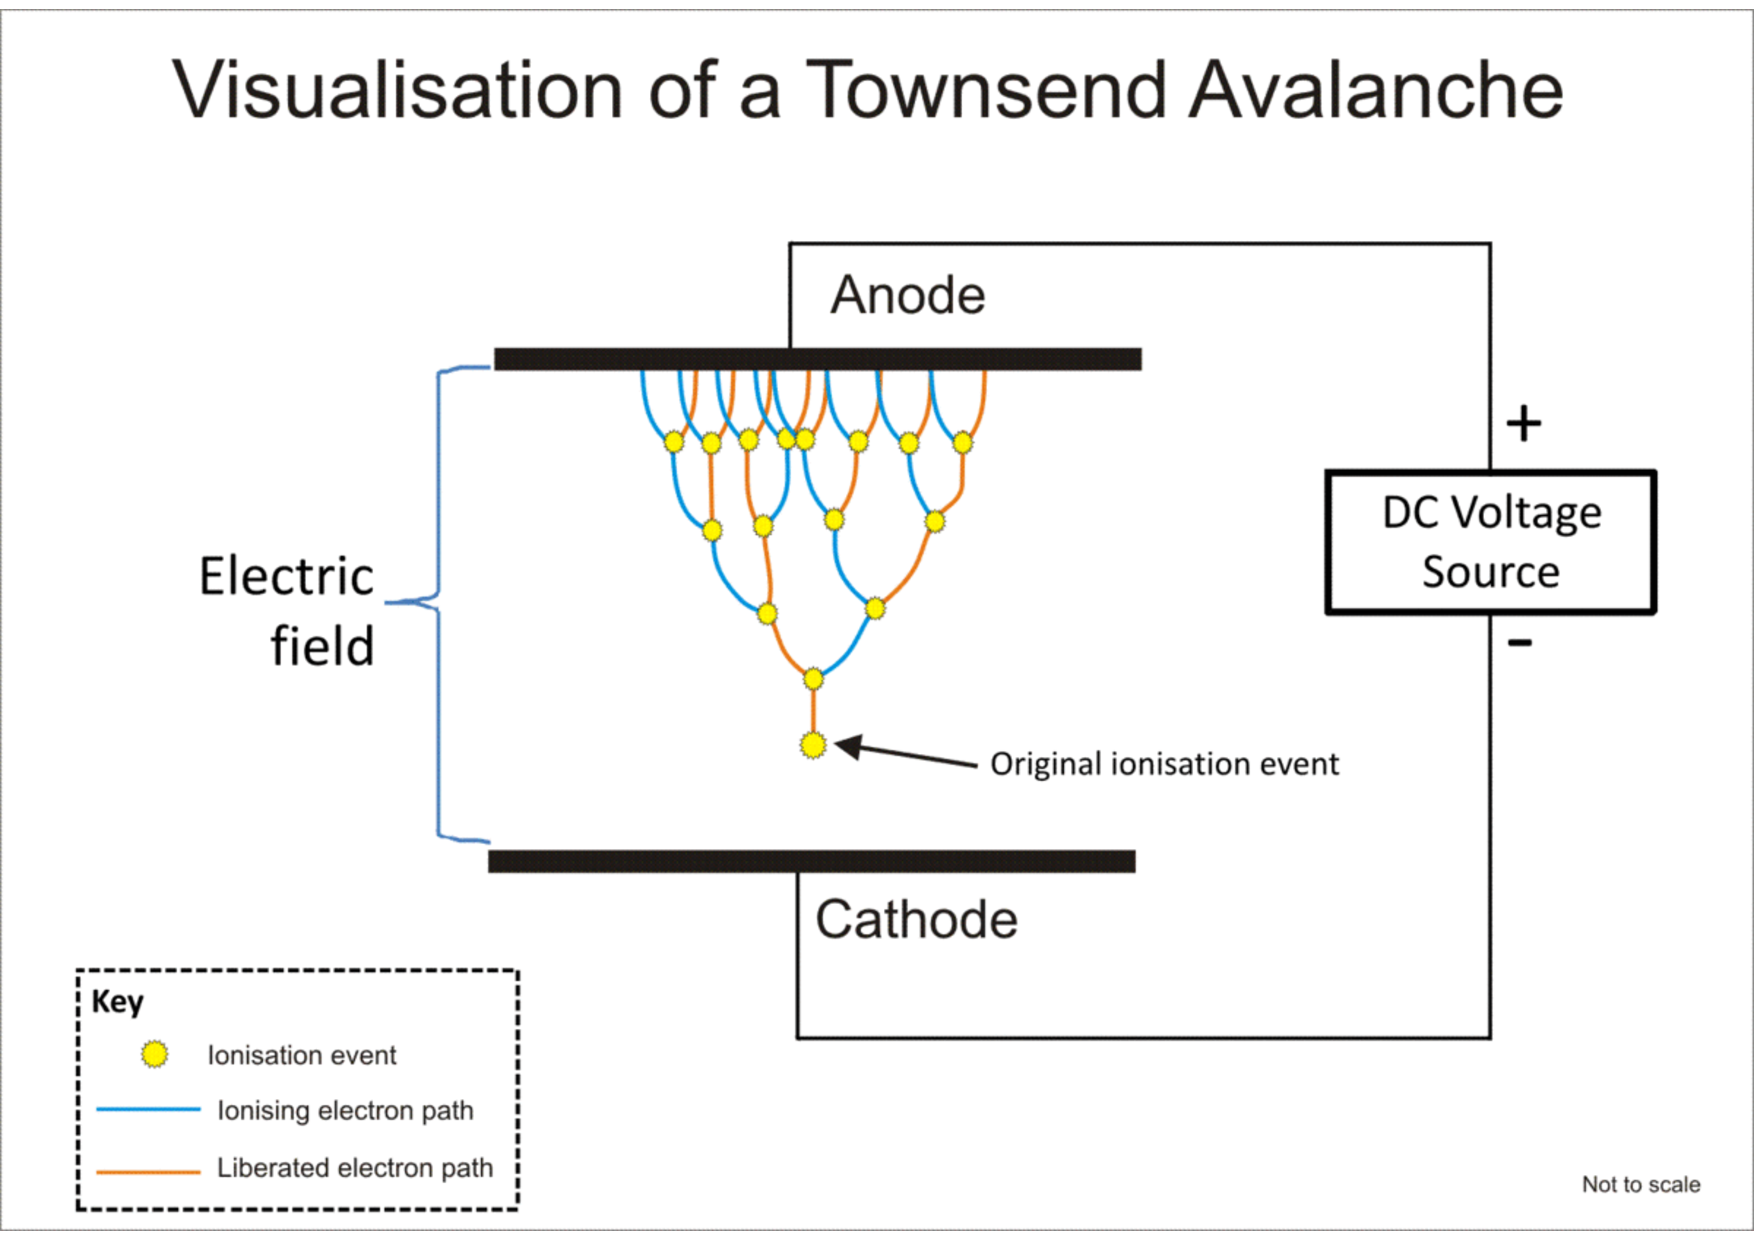
\includegraphics[width=.8\textwidth]{pics/avalanche}
\end{center}
\caption{When a gaseous medium is ionized by the track of a muon, 
the resulting liberated electrons are accelerated in the electric field and collide with gas molecules. The result is an 
avalanche of electrons collected at the anode. The process is known as a Townsend Avalanche.}
\label{fig:avalanche}
\end{figure}

\begin{figure}
\begin{center}
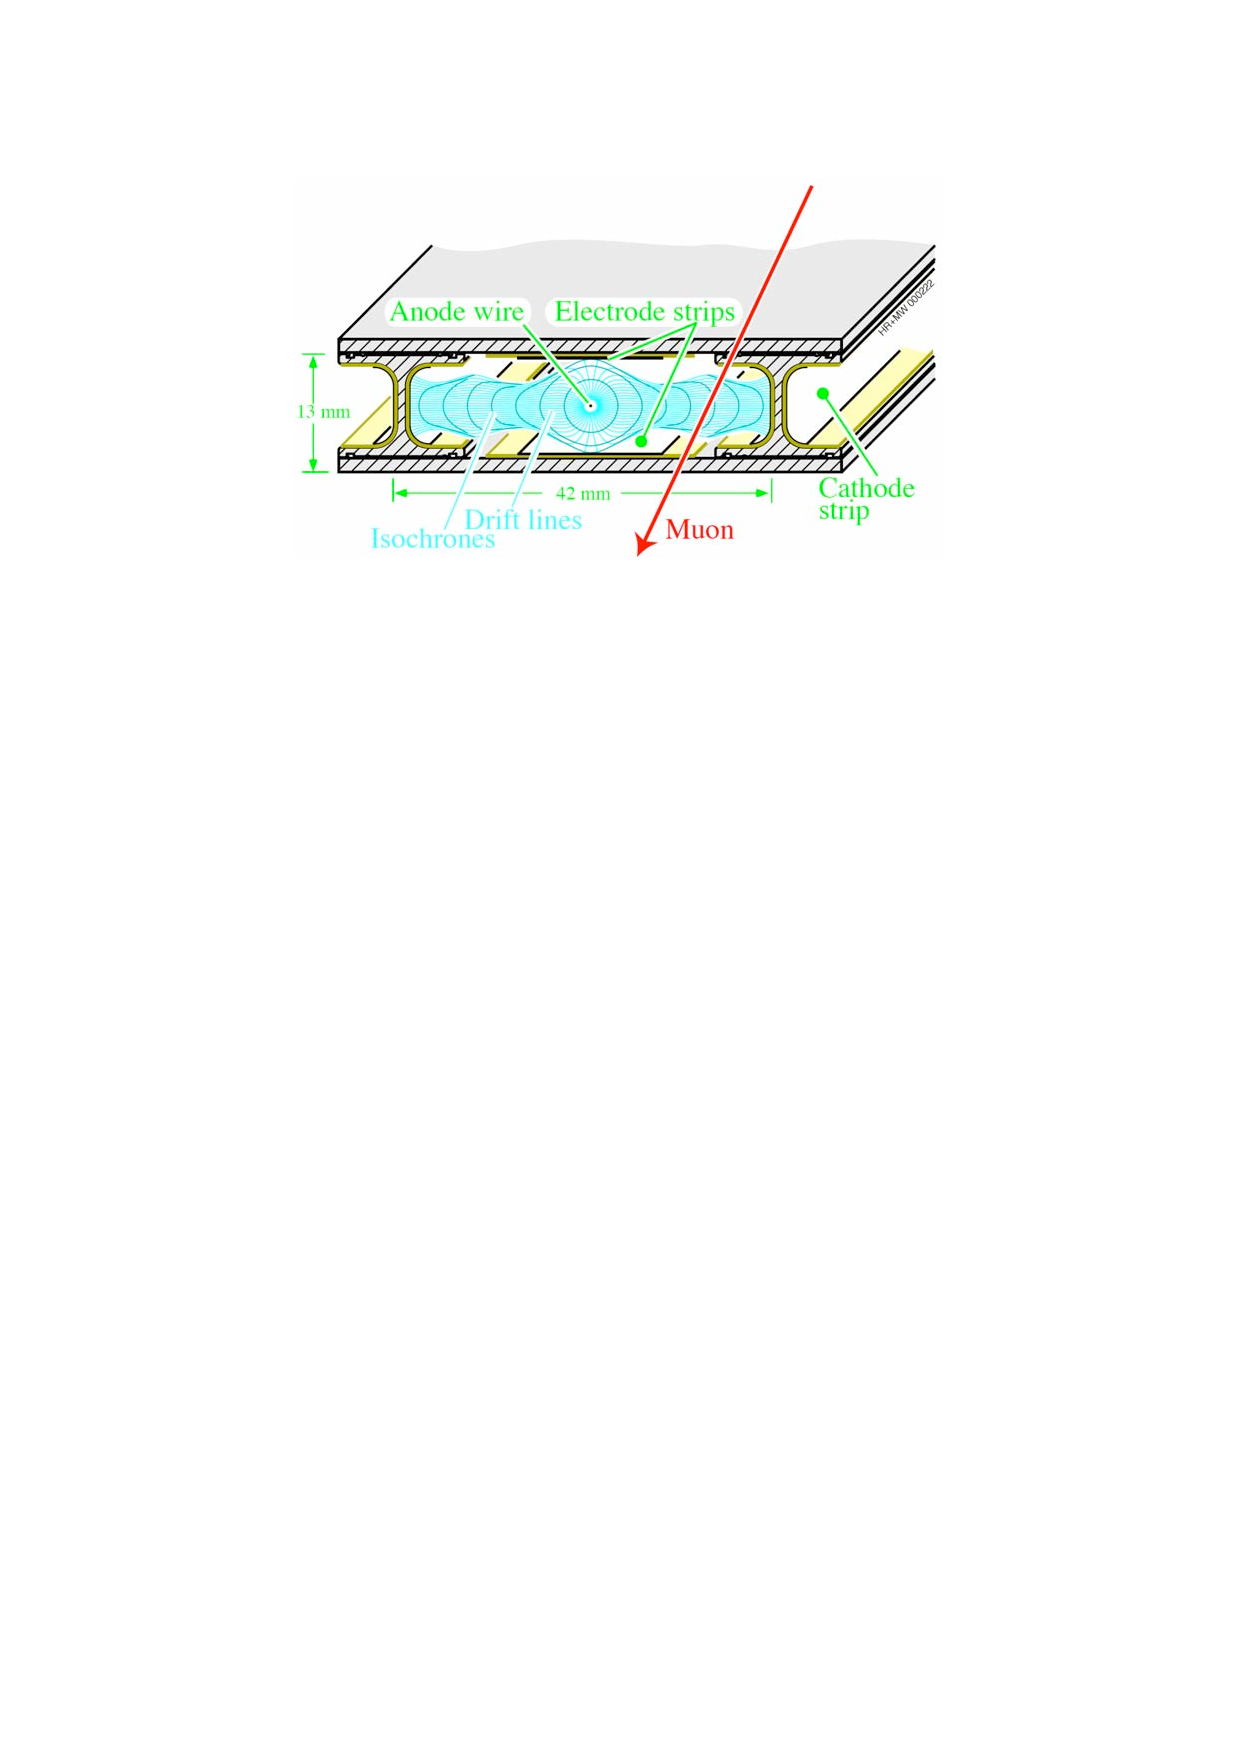
\includegraphics[width=.7\textwidth]{pics/cell_diagram}
\end{center}
\caption{The drift tube design showing the drift lines, wire, and cathode strips.}
\label{fig:cell}
\end{figure}

The Compact Muon Solenoid's name is partly taken from the muon subsystem which is
built to identify and measure the trajectories of muons. This thesis uses
only calorimeter quantities and inner tracking with correspondingly no sensitivity to muons.
This section is included only for completeness.  

The muon system consists of 3 separate detectors: drift tubes (DT's), resistive plate chambers (RPCs), and 
cathode strip chambers (CSCs). All three systems rely on the ionization of a gas medium caused by the charged muon's
traversal through the detector. The detectors are multi-layered and sandwiched between between layers of the iron  return
yoke (Figure \ref{fig:muon_diagram}). The iron layers aid in particle identification by stopping nearly all
 other particle activity before the final detector layer. As  muons are very weakly interacting, they should be the only
particles reaching the edge of the detector. When the magnetic field changes outside of the solenoid, muon tracks
will change curvature in the muon system as depicted in the CMS logo (Figure \ref{fig:muon_slice}). The second measurement
made in the muon spectrometer improves the momentum resolution for energetic muons $>100$ GeV, however lower momentum muons are dominated by a increase of multiple scattering from the additional detector material. 

It the context of long-lived searches it is interesting that the muon has a lifetime of $\tau_0=2.2$ $\mu$s or equivalently $c\tau_0 = $ 660 m. The dominant decay to an electron and two neutrinos  is suppressed by requiring the muon decays off-shell through the much heavier $W^{\pm}$. 
This method of generating long-lived signatures mirrors the motivations of
split supersymmetry where the gluinos are long-lived because they must decay through much heavier squarks.
If this were the end of the story we would expect $\approx$ 1\% of muon decays to occur before the final layer.  However, a moderately energetic muon will experience time dilation $c\gamma\tau_0$ in the lab frame with 
$\gamma = E / m = (1$ GeV$)/ 105$ MeV $\approx 10$. Accordingly, on detector length scales $O(10$ m$)$ energetic muons can be considered stable. 

The drift tube system located in the barrel region covers $|\eta| < 1.2$ with 4 concentric rings (segmented in $r=4.0,4.9,5.9,7.0$ m) referred to as ``stations''. Five divisions are also made in 
the $z$ direction referred to as ``wheels'' partitioned into 12 sectors of 30 degrees.  The three inner cylinders have 
60 chambers each and the outer cylinder has 70.   Each chamber measures 3.0 m $\times$ 2.5 m.
 Each chamber is divided into 3 (or 2) super layers with 4 drift cells per layer 
(2 in $\phi$, 2 in $z$). The drift cells
use anode wires at voltage of $+3.6$ kV, electrode strips at 1.8 kV and -1.2 kV cathode strips  to detect the localized ionization showers from muon tracks (Figures \ref{fig:avalanche} and \ref{fig:cell}). The full system includes 172,000 wires.  The maximal drift path
 is 21 mm corresponding to a drift time of 380 ns in a gas mixture of 85\% Argon and 15 \% CO$_2$ \cite{cmsexpcomplete}.

A combination of CSCs and DTs are located in the endcap region. The CSCs are located between $0.9 < |\eta| < 2.4$ and the RPCs between $0.9 < |\eta| < 1.6$. There are 4 stations for each endcap. The CSCs
 are trapezoidal multi-wire proportional chambers comprised  of 6 wire planes interleaved with 7 cathode panels. The chambers
 extend 1.7 (or 3.4) m in the radial direction covering 10 (or 20) degrees. Wires running in the $\phi$ direction define
 a tracks radial position. The $\phi$ coordinate along the wires is obtained by interpolating charges induced 
on the cathode strips. 

All four DT layers and multiple CSC layers include RPCs , which have a coarse position resolution
(order $\sim$1 cm) relative to the CSC and DT layers, but a much faster response time of ~3 ns.
This allows the RPC's to identify the bunch crossing of a muon unambiguously as well 
as aide in triggering on muon events. Each layer of the RPC is built from two resistive
 plates separated by a gap of freon gas held at a 9.5 kV.
Electrons knocked from the gas atoms cause an electron avalanche picked up by detector strip. The 
strip pattern gives a measure of momentum.

\begin{figure}
\begin{center}
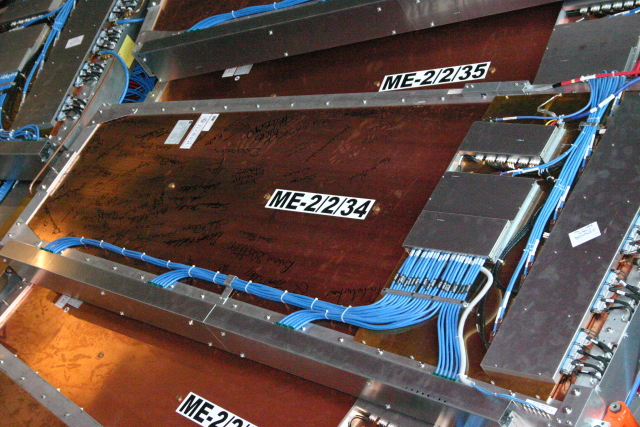
\includegraphics[width=.45\textwidth]{pics/cathode_strip_chamber}
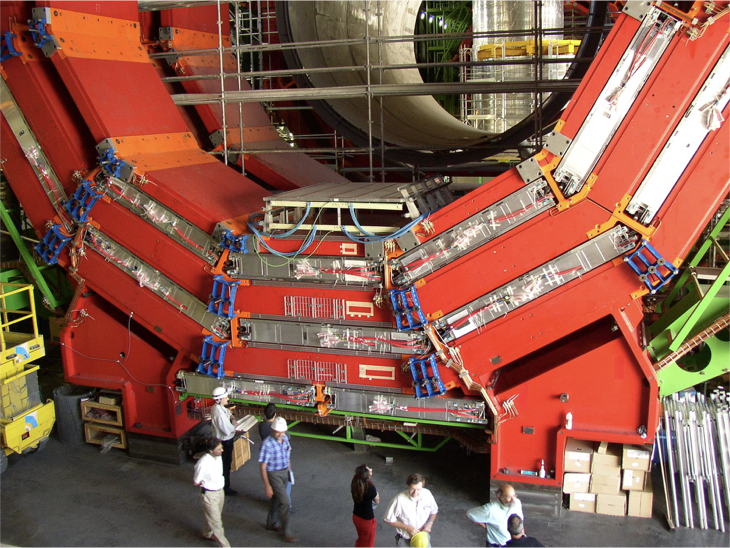
\includegraphics[width=.45\textwidth]{pics/rpc_plates}
\end{center}
\caption{The Muon cathode strip chamber.}
\label{fig:strip_chamber}
\end{figure}

\section{Trigger System}

\begin{figure}
\begin{center}
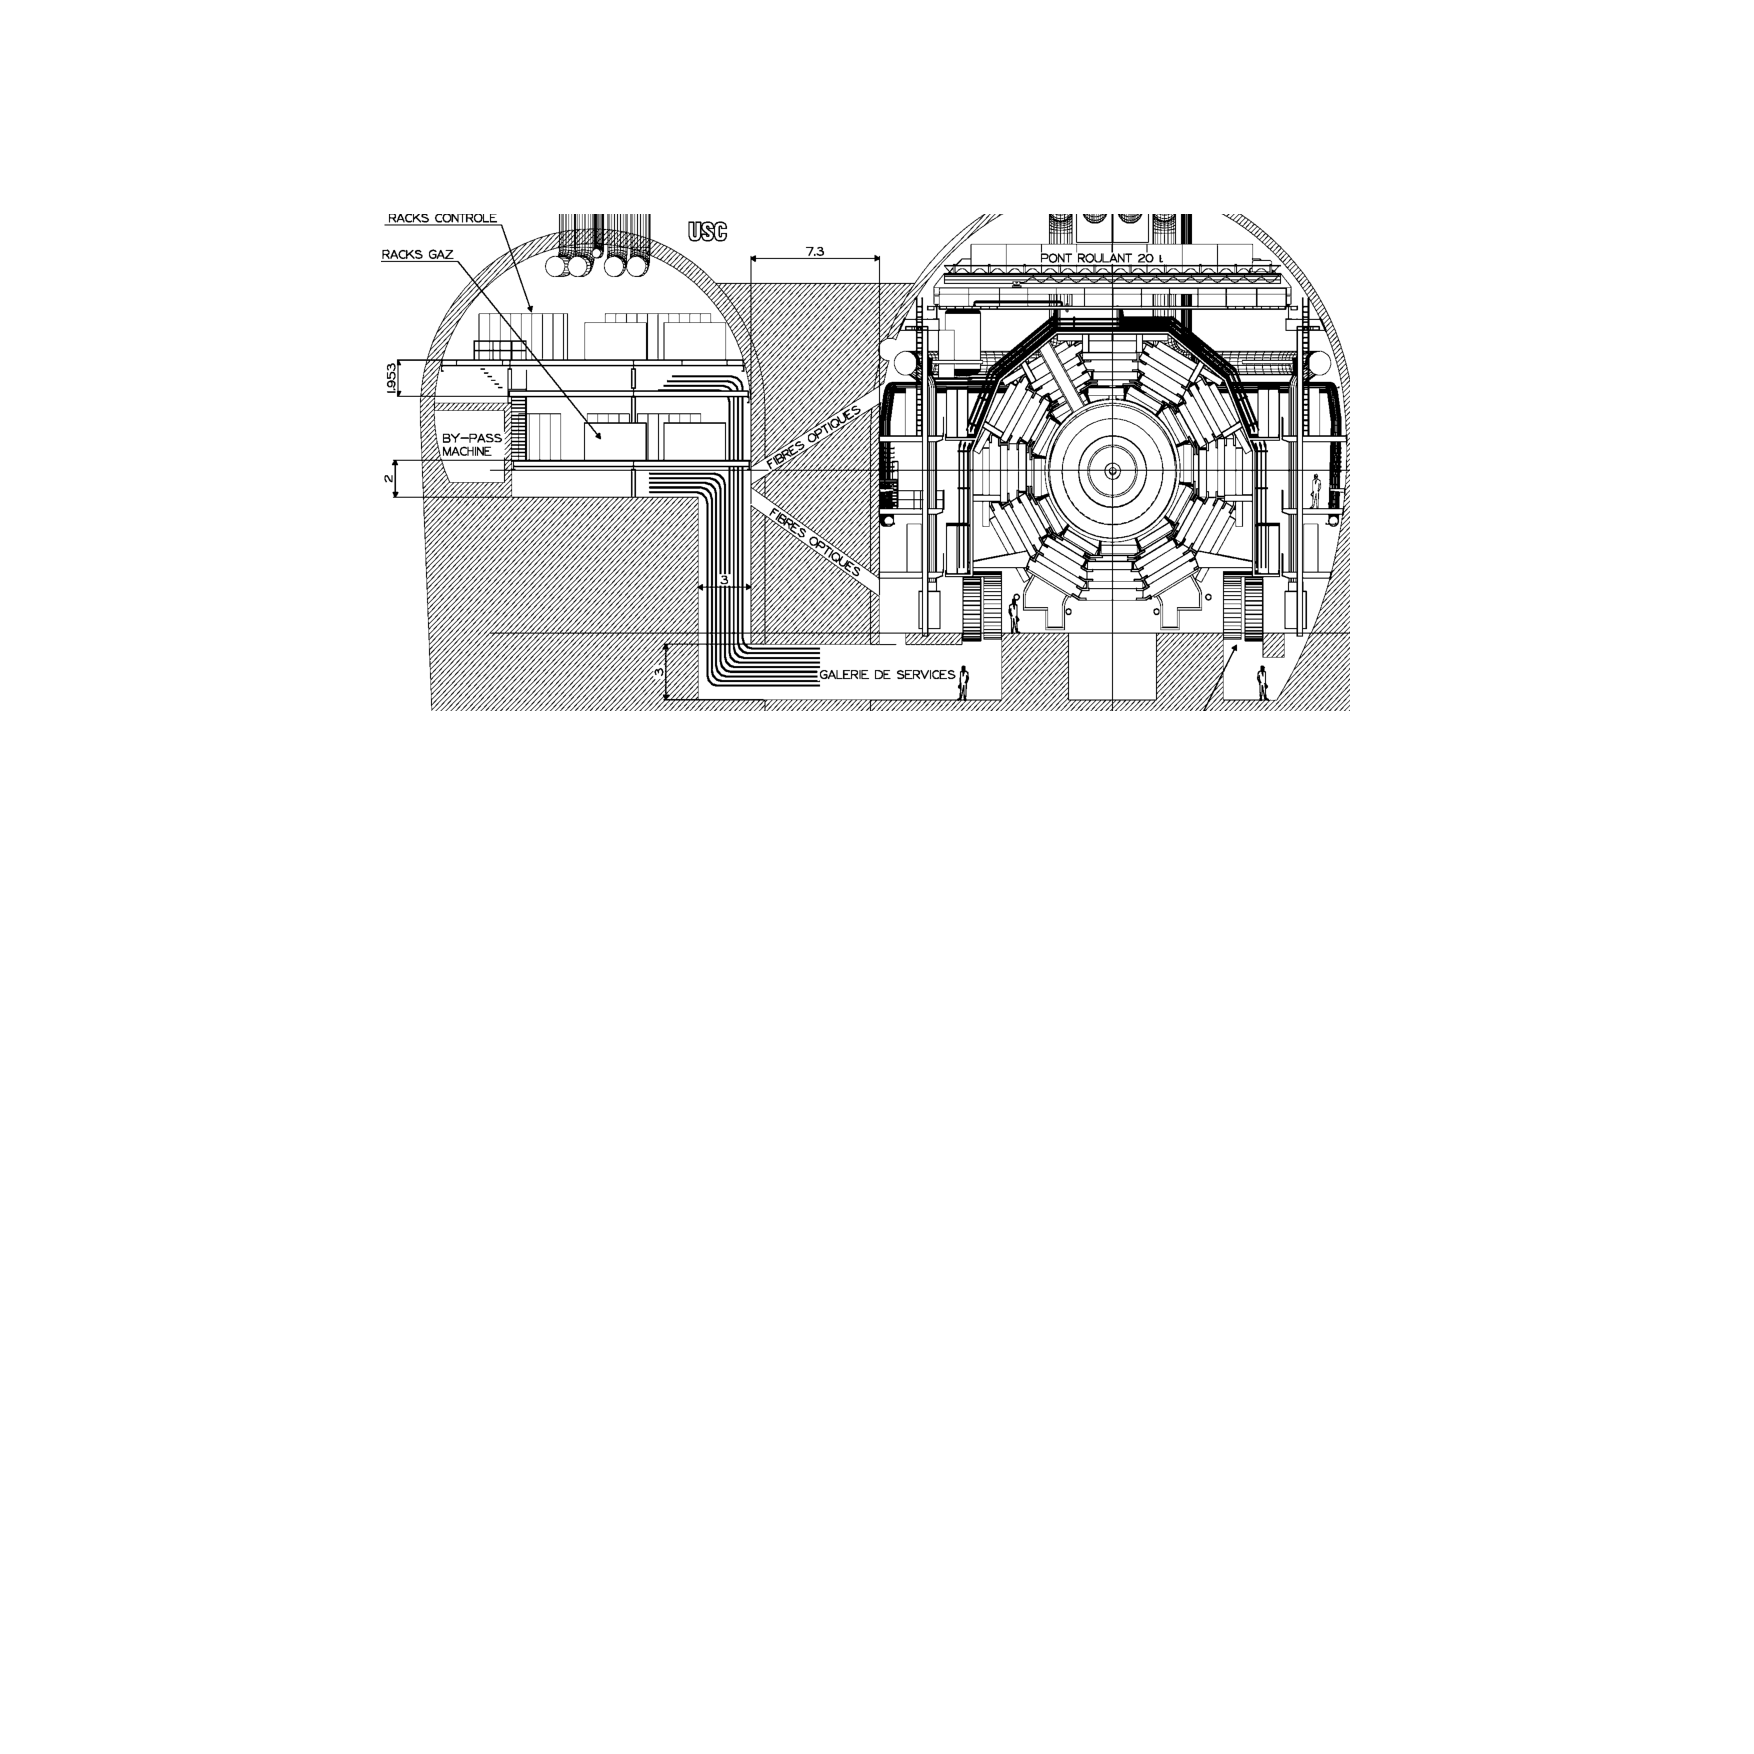
\includegraphics[width=.95\textwidth]{pics/counting_room}
\caption{The location of the counting room relative to the experimental hall.}
\end{center}
\label{fig:counting_room}
\end{figure}

\begin{figure}
\begin{center}
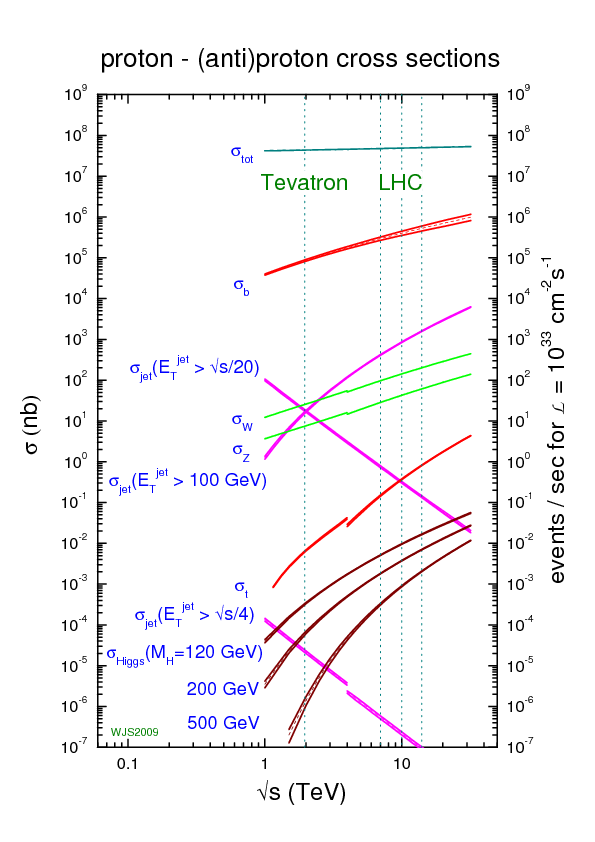
\includegraphics[width=.6\textwidth]{figures/exp_proj/pdf_xsec.png}
\end{center}
\caption{Common cross sections of proton collisions as a function of the center of mass energy $\sqrt{s}$.\label{fig:pdfxsec}}
\end{figure}

The CMS trigger system exists as a filter through which events are determined to be interesting or 
useful enough to be written to mass storage. The name comes from the nature of algorithms used to determine 
what to write down. If an event passes any of the online algorithms, this ``triggers'' the collision to be 
written in its entirety regardless of the goals of the path in particular 
 (albeit with some notable exceptions). It is both  unnecessary and impractical to record every
collision the LHC delivers. The low momentum transfer  hadronic events contained in the vast majority of
 proton collisions is well understood from past experiments. Figure \ref{fig:pdfxsec}  shows 
typical physics processes for proton-proton scattering. Events such as the production 
of a $b$ quark  occur at $\approx 10^6$ Hz at a luminosity of $\mathcal{L} = 10^{33}$ cm$^{-2}$ 
whereas processes of interest, such as the production of the Higgs is much lower at $\approx 10^{-2}$ Hz.  

The LHC has beam crossings at a rate of $\approx 40$ MHz. The number of inelastic collisions per bunch cross crossing
 is given by the  is the total inelastic cross section times the luminosity divided by the bunch collision rate. If every bunch is filled, this 
is respectively $8.5\times 10^{-26}~\text{cm}^2 \times 10^{34}~\text{cm}^{-2}~\text{s}^{-1}/ (40 \times 10^6~\text{s}^{-1}) \approx 24$ interactions.
The collisions are stored with an average file size O(1 MB) in their unprocessed 
form in a format referred to as RAW. However the bandwidth for the combined constraints of
 acquisition rate, storage and processing, is limited to $10^3$ Hz and equivalently $10^3$ MB/s. 
The trigger must be able to select these events quickly while maximizing the
 physics collected by the experiment with limited bandwidth.  

\begin{figure}
\begin{center}
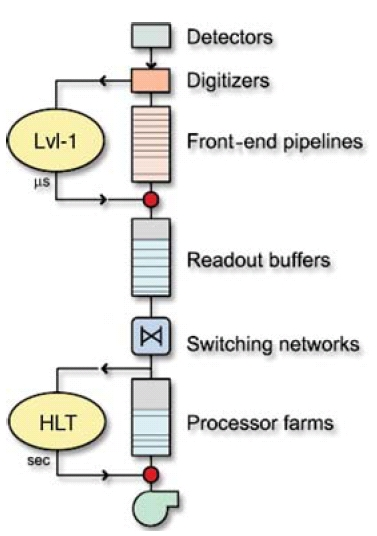
\includegraphics[width=.4\textwidth]{figures/exp_proj/cms-trigger}\\
\caption{The L1 and HLT trigger processing chain \cite{tridastdr}.}
\label{fig:l1_hlt_diagram}
\end{center}
\end{figure}

The CMS trigger system is designed to read events at the event crossing frequency and generate the
 factor $10^5$ of rejection between the crossing frequency and the archival capacity. This factor 
is too large to achieve in a single step given the complexity of triggers and event reconstruction necessary
to build fast algorithms. Therefore the task is split into two steps the Level 1 (L1) and High Level
 (HLT) Trigger systems (Figure \ref{fig:l1_hlt_diagram}). The L1 system is a coarse study of an event designed
to be fast and capable of analyzing every event at 40 MHz. The HLT provides the flexibility the L1 lacks 
permitting more elaborate event reconstruction. 

%% The $O(10^7$) events per second first pass through the L1 Trigger which reads out events at $10^5$ Hz. 
%% From here, the High Level Trigger makes the final decision as to which events are kept. 
%% Approximately 350 Hz is processed and stored, 300 Hz is ``parked'' (stored but processed later), 
%% and 1 kHz is partially stored (only the HLT level information and not the RAW detector information) 
%% and used for data scouting for future analysis.  

The simplest criterion for interesting events are hard physics events with large high momentum transfer, $q^2$, and
correspondingly large transverse momentum.
 As the protons collide with effectively no transverse momentum, significant deposits of 
transverse energy (or even missing transverse momentum) is indicative of a hard physics process. 
The total transverse energy of an event falls off exponentially, so a simple way to
reduce the rate of processed events is to raise the energy requirements of accepted events. However,
given the increasing luminosity of the LHC the thresholds are encroaching upon Standard Model physics processes
like single $W$ production, where triggering on most $W\rightarrow e\nu$ events is a reaching a kinematically limited regime. 

Generally, analyses searching for new physics are categorized by their final state signature.
Correspondingly, the triggers require loose particle identification 
on the particular objects such as the isolation and energy deposition. 
Requirements such as the angular separation, or the invariant mass of two objects is common as well.
Once the event has passed the  L1 and HLT Triggers, tighter and more computationally 
costly selection can be made offline where we are unrestricted by bandwidth limitations. 

\subsection{Level 1 (L1) Trigger}

The L1 Trigger is built using custom hardware composed of field programmable gate arrays (FPGAs), 
application-specific integrated circuits (ASICs) and programmable look up tables (LUTs). 

The trigger primitive generators (TPGs) are locally constructed from the energy deposits in the calorimeters or
hits/ track-segments in the muon chambers. The regional reconstruction applies coarse pattern
 recognition to the primitives and combines them. Together the  global calorimeter trigger (GCT)
 and global muon trigger (GMT) are processed at the global trigger (GT) to decide whether or
 not an event is kept. There is no inner tracking performed at this
 level (only muon specific tracking). Track building is time intensive and cannot, in its current
 state, be performed reliably at speeds comparable to the bunch crossing frequency. 
 Future upgrades are planned to include tracking at L1, which would significantly aide in
 the detection of soft hadronic signatures with specific track topologies (eg. displaced signatures 
 and VBF Standard Model Higgs production in decays to $b\bar{b}$). 

\begin{figure}
\begin{center}
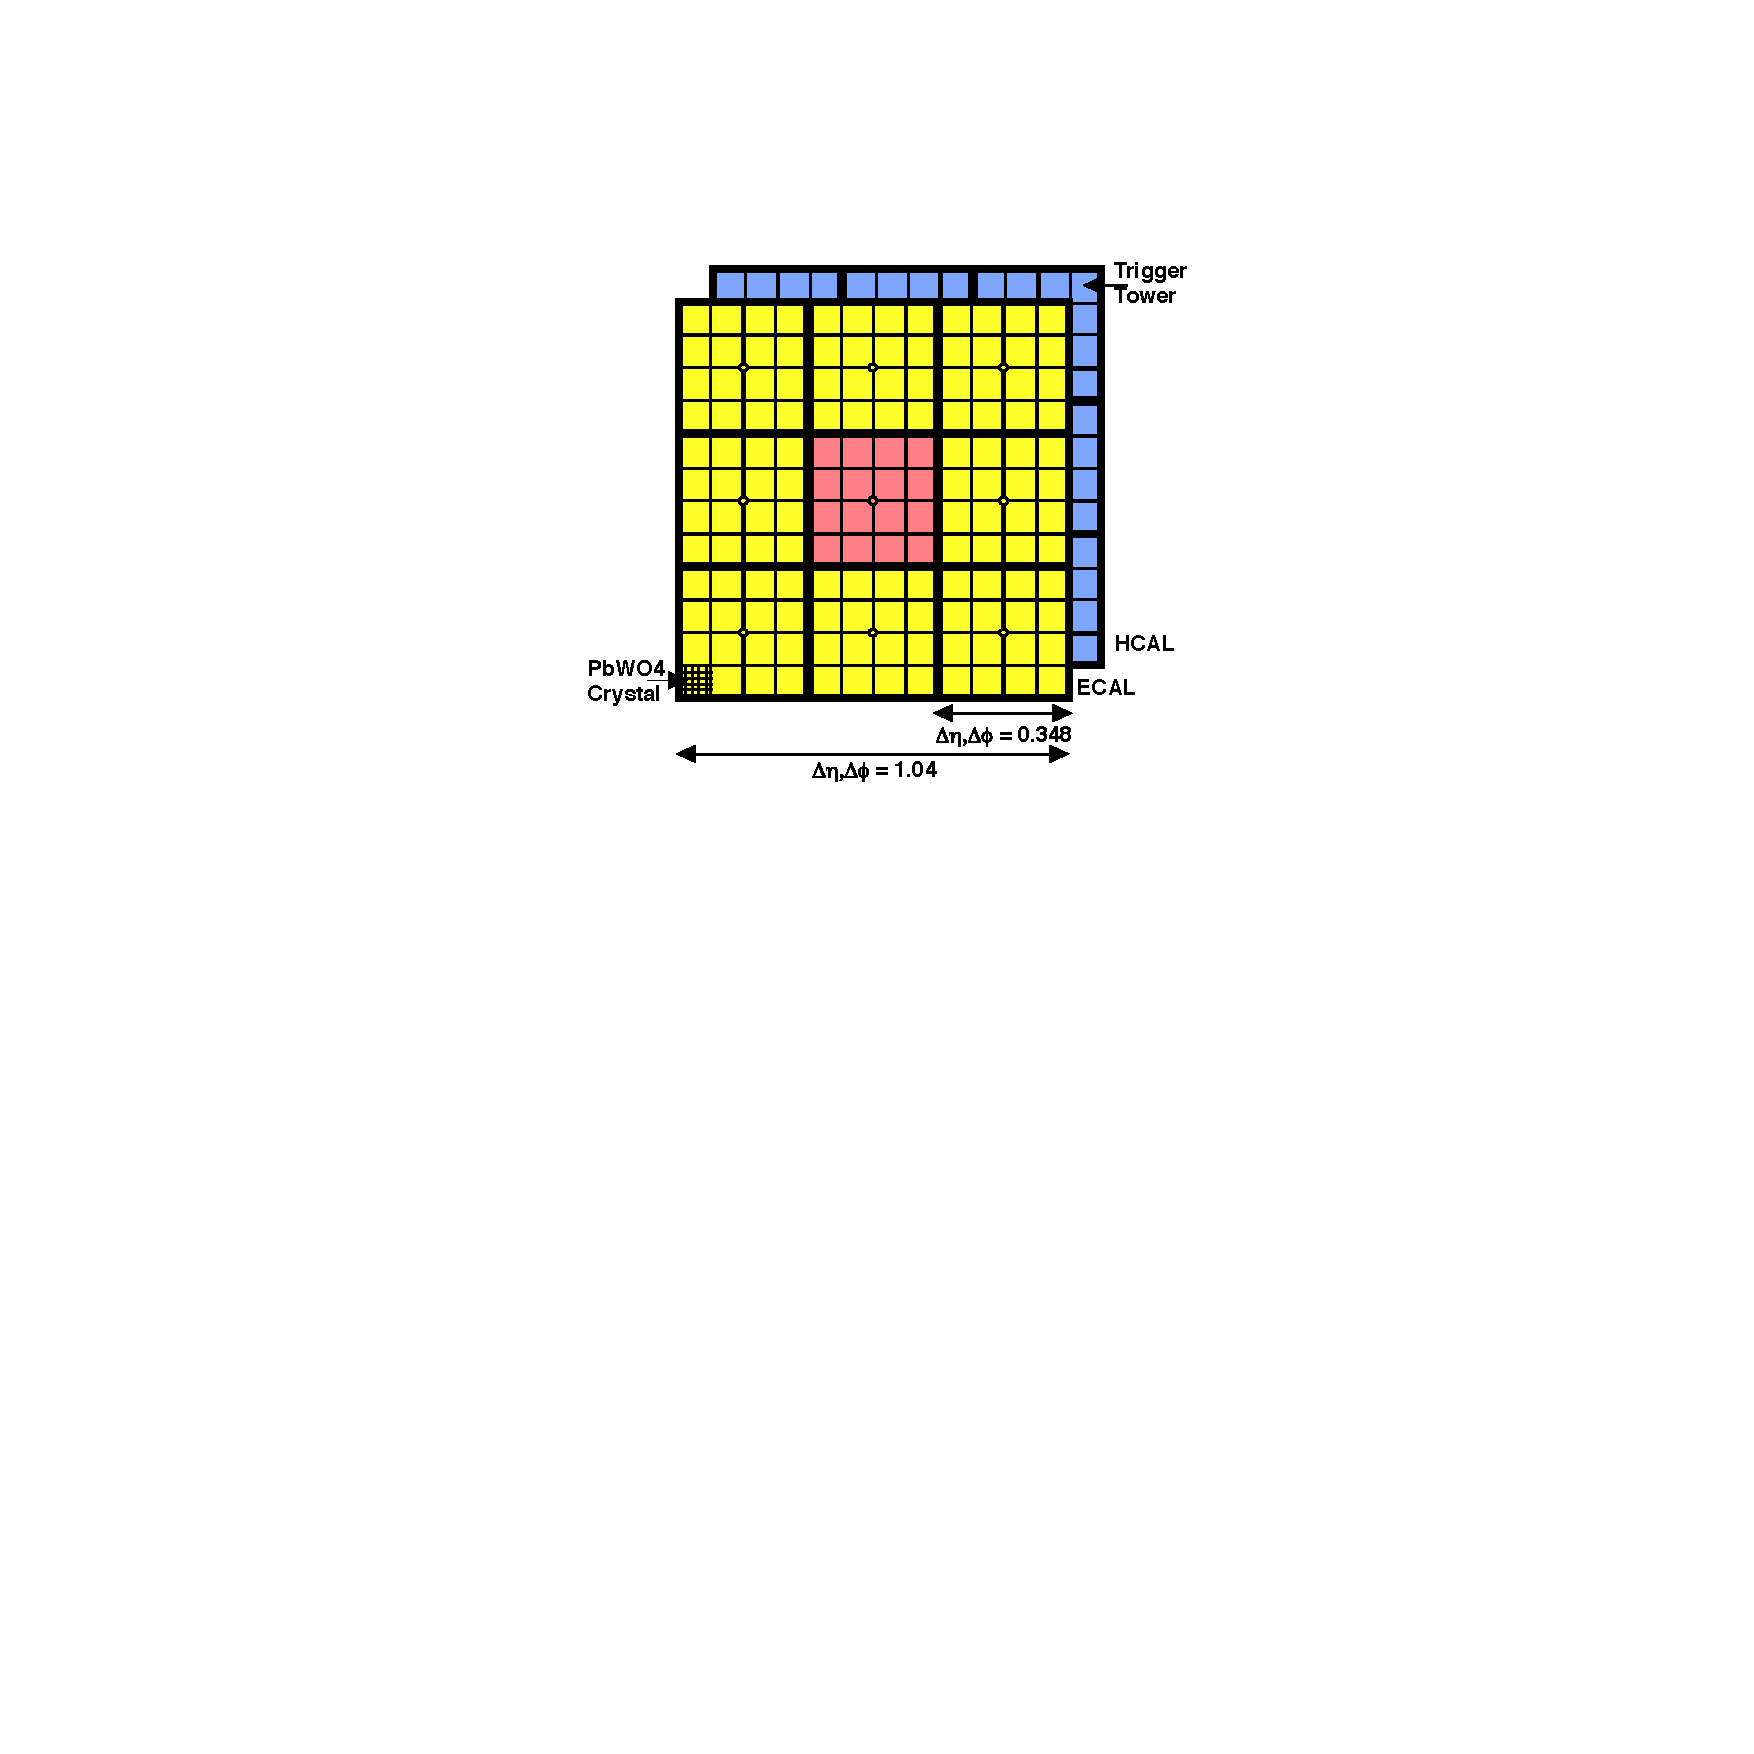
\includegraphics[width=.55\textwidth]{pics/jet_trigger_tower}
\caption{A  representation of a jet as assembled from the ECAL and HCAL trigger primitives. \cite{tridastdr}}
\end{center}
\label{fig:jet_trigger_tower}
\end{figure}
%The jet trigger primitives are built from transverse regions of 12 x 12 grids (Figure \ref{fig:jet_trigger_tower}) 
%% The regional calorimeter trigger (RCT) collects regional transverse energy sums segmented in variable size
%%  trigger tower arrays summed between the ECAL and transversely adjacent HCAL within $|\eta| < 5.0$. Electrons
%% and photons use the same size 

\subsection{High Level Trigger (HLT)}

\begin{center}
\begin{table}[]
\begin{center}
\caption{High Level Trigger filter farm configuration in 2015 \cite{timing}}
\begin{tabular}{cccc}
Install Year: & 2011 & 2012 & 2015 \\  
\hline
CPU & X5650  & E6-2670  & E6-2680v3  \\
Architecture & Westmere  & Sandy Bridge & Haswell \\
CPUs per board & 2 & 2 & 2 \\
Cores/CPU & 6 & 8 & 12 \\
RAM & 24 GB & 32 GB & 64 GB \\
Clock Rate (w/Boost) & 2.66 (3.06) GHz & 2.60 (3.30) GHz & 2.50 (3.30) GHz \\

Total Cores (Boards) & 3456 (288) & 4096 (256) & 8640 (360) \\ 
\end{tabular}
\end{center}
\end{table}
\end{center}


Algorithms at trigger stage are referred to as paths. The entire collection of paths is referred to
 as a trigger menu. As the physics goals of the experiment change and machine luminosity ramps, 
the menu must evolve and adjust the thresholds within a given menu. The HLT is a crucial component of 
CMS data taking, as new physics that is never stored is never discovered. Problems with the offline
 reconstruction can be fixed at a later date by reprocessing the raw data, but problems with the online reconstruction 
will permanently bias the data collected. 

The paths are configured as a series of reusable modules that either build some quantity/object (producers) 
or terminate the execution of the path based on some quantity (filters). The paradigm ensures, that a producer which creates, say, the sum of transverse energy in the detector, is processed exactly once despite being used by multiple paths. Ensuring that modules are reusable and reused greatly minimizes timing overhead of additional
paths. Common sequences, such as unpacking the calorimeter energy, are utilized by nearly every trigger. 
CMS as an experiment excels from a monolithic approach to software, where the same software (known as CMSSW) is
 for analysis and data processing is used online.

\begin{figure}
\begin{center}
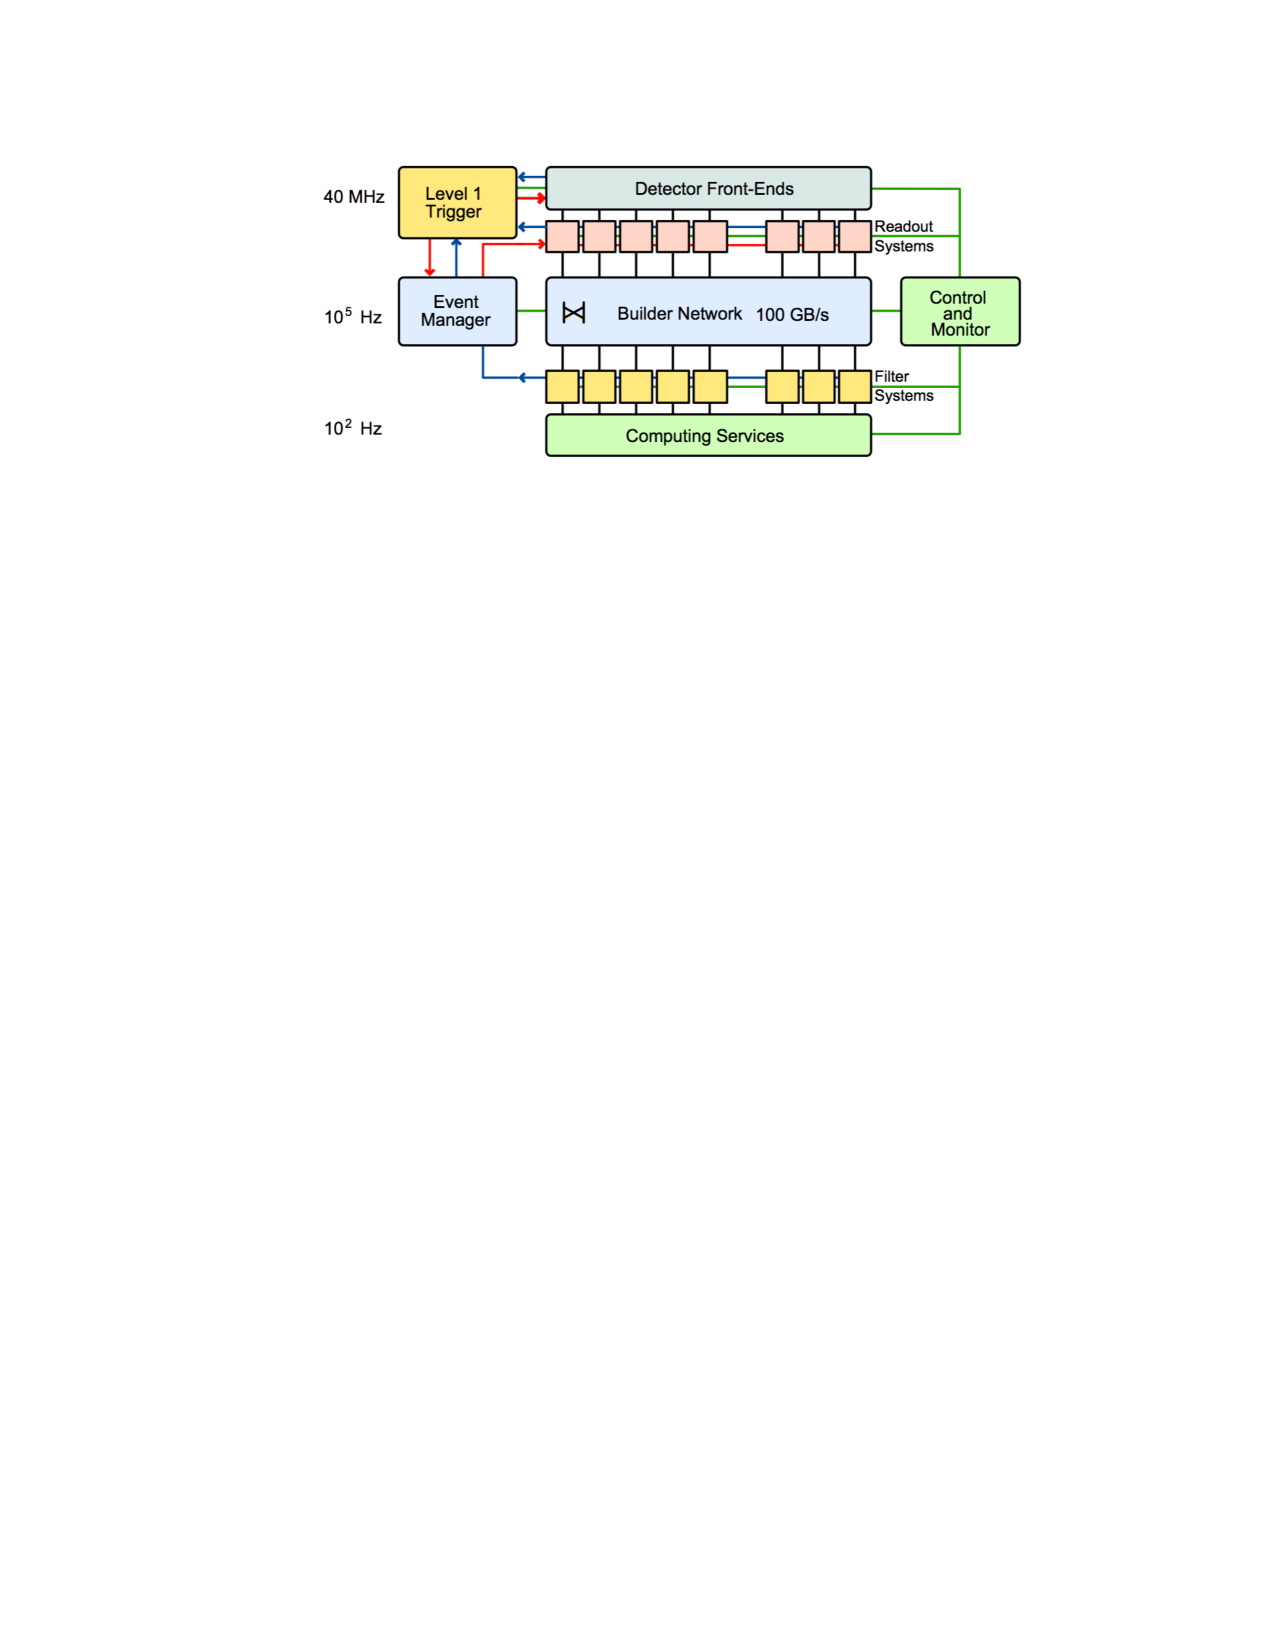
\includegraphics[width=.95\textwidth]{pics/daq_diagram}\\
\caption{A diagrammatic representation of the level 1 and HLT trigger processing}
\label{tab:daq_diagram}
\end{center}
\end{figure}

The development, debugging, and testing of these menus
is a large organizational effort that requires input from nearly every level of the experiment. 
Physics object groups (POGs):  e/$\gamma$, muons, jets, and b tagging group must build
the online recommendations for object identification and vaildate their performance.
 Physics Groups (Higgs, Exotica, SUSY, ect.) must develop paths and justify the
added physics value of the individual paths in terms of their sensitivity. The detector performance groups (DPGs) 
must provide  calibrations for the online reconstruction that will differ from
the offline reconstruction. 

Additionally, the DPGs must implement separate data streams, which save a much
smaller event content, to calibrate the detector. For instance a separate data stream exists for collecting
the copious production of $\pi^0$ and $\eta^0$ mesons which predominantly decay to two photons. The stream 
performs only the reconstruction of the ECAL and searches for low $p_t$ clusters within an invariant mass window. 
Saving only the hits corresponding to these clusters reduces the event size from 1 MB to 2 kB allowing the stream
to acquire events at a rate of 7 kHz while maintaining a small bandwidth. For comparison, the physics data 
stream writes at 1 kHz. 

The CMS HLT System is built from a varied collection of commercially
 available CPUs  comprising more than 16,000 cores  in 2015 (Table \ref{tab:daq_diagram}). 
